\documentclass[12pt, oneside]{article} 
\usepackage{amsmath, amsthm, amssymb, calrsfs, wasysym, verbatim, bbm, color, graphicx, geometry, fancyhdr, url, multirow, hyperref, enumitem, comment, float, array, longtable, verbatim, array}
\usepackage[italian]{babel}

\geometry{tmargin=.75in, bmargin=.75in, lmargin=.75in, rmargin = .75in}


\author{RAMtastic6}

%Intestazione
\pagestyle{fancy}
\fancyhf{}
\fancyhead[R]{Gruppo 14 RAMtastic6\\ramtastic6@gmail.com}
\fancyfoot[C]{\thepage}

% Linea intestazione
\renewcommand{\headrulewidth}{1pt} 

% Intestazione documento
\begin{document}
% Salta la prima pagina per l'intestazione
\thispagestyle{empty}
\title{Analisi Dei Requisiti}
\maketitle
\begin{figure}[h]
  \centering
  
\includegraphics[scale=0.3]{logo.png}
\end{figure}
\begin{center}
    email: ramtastic6@gmail.com
\end{center}

% Informazioni sul documento
\section*{Informazioni sul documento} 
\begin{tabular}{ll}
Versione: & 3.0.0 \\
Redattori: &  Visentin S.  Zaupa R. Brotto D. Basso L. Zambon M. Tonietto F. \\ 
Verificatori: & Tonietto F. Visentin S. Brotto D. Zaupa R. Zambon M.\\
Destinatari: & Vardanega T., Cardin R., Imola Informatica \\
Uso: & Esterno
\end{tabular}
\newpage

% Registro dei cambiamenti
\section*{Registro dei Cambiamenti - Changelog}
\begin{longtable}{|c|c|c|c|p{7cm}|}
\hline
\textbf{Versione} & \textbf{Data} & \textbf{Autore} & \textbf{Verificatore} & 
\textbf{Dettaglio} \\
\hline
v 3.0.0 & 2024-04-29 & Zambon M. & Zambon M. & Approvazione e verifica del documento\\
\hline
v 2.3.0 & 2024-05-31 & Brotto D. & Zambon M. & Allineati i requisiti funzionali secondo i requisiti stilati nel documento di Specifica Tecnica: corretti i testi di ROF4 e RDF44; cambiati requisiti funzionali 8,18,35,70,72 da obbligatori a desiderabili. \\
\hline
v 2.2.0 & 2024-05-15 & Brotto D. & Zambon M. & Aggiunto ROF 77 nella sezione requisiti. \newline Aggiunto ROF 77 nella tabella di Tracciamento Requisiti in UC5. \newline Aggiornati Requisiti Funzionali 5,7 da desiderabili a obbligatori. \newline Aggiornati Requisiti Funzionali 52,53,54,56,60 da obbligatori a desiderabili.\\
\hline
v 2.1.2 & 2024-05-13 & Basso L. & Zambon M. & Aggiunto ROF 76 nella sezione requisiti. \\
\hline
v 2.1.1 & 2024-05-13 & Basso L. & Zambon M. & Modificati UC24 e UC11; ora gli attori sono utenti generici. \\
\hline
v 2.1.0 & 2024-05-04 & Visentin S. & Zaupa R. & Modificati alcuni requisiti obbligatori in desiderabili (2, 17 , 21 ,22, 23 ,26 ,27 ,42 ,44 , 45,  47, 48, 59, 64, 65, 66, 73, 74) e aggiunto ROF 75\\
\hline
v 2.0.0 & 2024-04-29 & Visentin S. & Visentin S. & Approvazione e verifica del documento\\
\hline
v 1.2.0 & 2024-04-29 & Zambon M. & Tonietto F. & Correzione di alcuni punti secondo i $\textit{feedback}_G$ del prof. Cardin: modificati gli scenari principali, modificati i diagrammi e aggiunti $\textit{riferimenti}_G$ in UC4 e UC30\\
\hline
v 1.1.1 & 2024-04-28 &   \begin{tabular}[c]{@{}c@{}}
    Basso L. \\
  \end{tabular}  & \begin{tabular}[c]{@{}c@{}}
    Tonietto F.
  \end{tabular} & Correzione di alcuni punti secondo i $\textit{feedback}_G$ del prof. Cardin: inserimento diagrammi UC1, UC2 e UC3; approfondimento di UC3.1 e aggiunta del diagramma associato ad esso.\\
\hline
v 1.1.0 & 2024-04-27 &   \begin{tabular}[c]{@{}c@{}}
    Tonietto F. \\
  \end{tabular}  & \begin{tabular}[c]{@{}c@{}}
    Visentin S.
  \end{tabular} & Correzione di alcuni punti secondo i $\textit{feedback}_G$ del prof. Cardin: rettifica funzionamento di UC23; rielaborazione $\textit{precondizioni}_G$ UC7; rielaborazione UC8 e UC8.1; correzione $\textit{UML}_G$ di UC11; aggiunta di Requisiti di Vincolo\\
\hline 
v 1.0.0 & 2024-04-06 &   \begin{tabular}[c]{@{}c@{}}
    Zaupa R. \\
    Brotto D. \\
  \end{tabular}  & \begin{tabular}[c]{@{}c@{}}
    Zaupa R. \\
    Brotto D. \\
  \end{tabular} & Approvazione e validazione del documento\\
\hline
v 0.6.1 & 2024-04-05 & Zambon M. & Zaupa R. & Cambiati alcuni termini che sono presenti nel glossario per risolvere alcuni problemi con l’automazione dei riferimenti\\
\hline
v 0.6.0 & 2024-03-06 & Brotto D. & Filippo T. & Creato UC27 - Logout con relativi ROF (80,81,82) 
\newline Rimosso il vecchio UC30 e i suoi ROF, su decisione che admin può amministrare solo 1 ristorante
\\
\hline
v 0.5.5 & 2024-03-06 & Zaupa R. & Tonietto F. & Eliminato $\textit{caso d'uso}_G$ UC9 "Ricerca pasti ordinabili". Aggiunto al suo posto nuovo $\textit{caso d'uso}_G$ "Modifica del proprio ordine". Inserito UC29 "$\textit{Ordinazione}_G$ piatto" come sottocaso di UC3. Aggiornato UC6 con nuovi diagrammi e nuovi sottocasi. Aggiunto UC28 "Annullamento dell'ordinazione". Aggiornata la sezione 4 "Requisiti" di conseguenza e aggiunti ROF 42-43-78-79. \\
\hline
v 0.5.4 & 2024-03-05 & Zaupa R. & Tonietto F. & Inserito diagramma per gli attori coinvolti (sezione 3.1), modificati casi d'uso ed inserito nuovo diagramma per UC14, UC15, UC17. Inseriti UC32 e UC33 come $\textit{sottocasi d'uso}_G$ di UC31 e sistemati i $\textit{riferimenti}_G$ nei requisiti. Inserita sezione 4.3 Tracciamento e tabella nella sezione 4.3.1\\
\hline
v 0.5.3 & 2024-02-29 & Brotto D. & Tonietto F. & UC25 e UC26 cambiati da "Inserimento" a "Modifica";
\newline Unificati UC5,6,9,11 dai loro sottocasi;
\newline Creati diagrammi UC19,20;
\newline Creati ROF:
\newline per UC26 (68,69,70)
\newline per UC29 (71,72,73)
\\
\hline
v 0.5.2 & 2024-02-28 & Brotto D. & Tonietto F. & Creati ROF:
\newline per UC17 (64,65) 
\newline per UC25 (66,67)
\\
\hline
v 0.5.1 & 2024-02-26 & Brotto D. & Tonietto F. & Corretto diagramma UC6 e creato diagramma UC16; \newline ROF: per UC2(45,46,47,56(new)); 
\newline Creati ROF: \newline per UC12(57,58,59); \newline per UC16(60,61,62,63); \\
\hline
v 0.5.0 & 2024-02-19 & Zaupa R. & Tonietto F. & Inserimento casi d'uso UC31-32-33 con i relativi diagrammi. Ridefinizione di UC11 (con relativo sottocaso d'uso) e UC14 con relativi diagrammi. Inseriti ROF dal 48 a al 50 e UC11 in ROF1. \\
\hline
v 0.4.2 & 2024-02-16 & Brotto D. & Tonietto F. & Inserimento requisiti funzionali di UC6, UC15, UC30, UC1 (da ROF 36 a 47), creazione UC30 con relativo diagramma \\
\hline
v 0.4.1 & 2024-02-15 & Zaupa R. & Tonietto F. & Inserimento requisiti funzionali di UC11 e UC18 (da ROF 33 a 35), inserimento scenari UC11.1, UC11.2, UC11.3, UC18; inserimento diagramma UC18 \\
\hline
v 0.4.0 & 2024-01-17 & Brotto D. & Tonietto F. & Scrittura requisiti funzionali di UC4 (da ROF 23 a 26 e UC4 aggiunto a ROF 13) \\
\hline
v 0.3.2 & 2024-01-14 & 
\begin{tabular}[c]{@{}c@{}}
    Davide B. \\
    Samuele V.
  \end{tabular} 
& Tonietto F. & Creazione e inserimento sezione requisiti funzionali. Da ROF 1 a ROF 13: Samuele; Da ROF 14 a ROF 22: Brotto\\
\hline
v 0.3.1 & 2023-12-20 & Zaupa R. & Tonietto F. & Inserimento diagrammi dei casi d'uso dal 4 al 7; revisione  UC6 e UC7, stesura sotto$\textit{caso d'uso}_G$ UC6.1 e $\textit{caso d'uso}_G$ UCE1; stesura casi d'uso UC21 e UC22 \\
\hline
v.0.3.0 & 2023-12-18 & Zambon M. & Brotto D. & Completata stesura $\textit{scenario}_G$ 2 con descrizione casi d'uso \\
\hline
v.0.2.2 & 2023-12-17 & Zambon M. & Brotto D. & Iniziata stesura $\textit{scenario}_G$ 2 con diagramma \\
\hline
v.0.2.1 & 2023-12-15 & Zambon M. & Brotto D. & Stesura $\textit{scenario}_G$ 1 con diagramma e descrizione casi d'uso \\
\hline
v.0.2.0 & 2023-11-28 & Basso L. & Visentin S. & Aggiunta dei casi d'uso da 19 e 20; modificato UC3 ($\textit{ordinazione}_G$ collaborativa) \\
\hline
v.0.1.0 & 2023-11-28 & Basso L. & Tonietto F. & Aggiunta ai casi d'uso da 1 a 2 delle estensioni (scenari secondari) \\
\hline
v.0.0.5 & 2023-11-27 & Visentin S. & Tonietto F. & Stesura casi d'uso 11 a UC18 \\
\hline
v.0.0.4 & 2023-11-25 & Visentin S. & Tonietto F. & Dichiarazione casi d'uso da UC14 a UC18 \\
\hline
v.0.0.3 & 2023-11-22 & Zaupa R. & Tonietto F. & Riorganizzazione del documento; stesura dei casi d'uso UC9 e UC10; dichiarazione dei casi d'uso da UC11 a UC13 \\
\hline
v.0.0.2 & 2023-11-21 & 
  \begin{tabular}[c]{@{}c@{}}
    Zaupa R. \\
    Visentin S.
  \end{tabular} 
  & Tonietto F. & Prima versione, stesura della sezione 1 (Introduzione) e prima stesura della sezione 3 (Casi d'uso), in particolare della sezione 3.1 (Attori) e dei casi d'uso da UC1 a UC8 con i relativi sottocasi\\
\hline
\end{longtable}
\newpage

% Sommario
\tableofcontents
\newpage

% Introduzione
\section{Introduzione}
\subsection{Scopo del documento}
Il presente documento ha lo scopo di delineare in maniera approfondita i casi d'uso e i requisiti del progetto $\textit{Easy Meal}_G$, come specificato nel $\textit{capitolato}_G$ d'appalto C3 per il corso di $\textit{Ingegneria del software}_G$ proposto dall'azienda $\textit{Imola Informatica}_G$.
L'analisi si basa sulla presentazione del $\textit{capitolato}_G$ seguita da incontri diretti con il proponente al fine di approfondirne gli aspetti chiave. Eventuali termini tecnici sono definiti all'interno del documento "Glossario Tecnico".
\subsection{Scopo del prodotto}
Il prodotto finale, realizzato tramite un'$\textit{Applicazione Web Responsive}_G$, si propone di realizzare un $\textit{software}_G$ innovativo volto a semplificate il $\textit{processo}_G$ di $\textit{prenotazione}_G$ e $\textit{ordinazione}_G$ nei ristoranti, contribuendo a migliorare l'esperienza per clienti e ristoratori. In particolare, $\textit{Easy Meal}_G$ dovrà consentire agli utenti di personalizzare gli ordini in base alle proprie preferenze, allergie ed esigenze alimentari; interagire direttamente con lo staff del ristorante attraverso una chat integrata; consentire di dividere il conto tra i partecipanti al tavolo.
\subsection{Riferimenti}
\subsubsection{Riferimenti normativi}
\begin{enumerate}
    \item Presentazione del $\textit{capitolato}_G$ d'appalto C3 - Progetto $\textit{Easy Meal}_G$: \\ \url{https://www.math.unipd.it/~tullio/IS-1/2023/Progetto/C3.pdf}
    \item Regolamento del progetto didattico: \\ \url{https://www.math.unipd.it/~tullio/IS-1/2023/Dispense/PD2.pdf}
    \item $\textit{Norme di Progetto}_G$ v2.0.0.
\end{enumerate}
\subsubsection{Riferimenti informativi}
\begin{enumerate}
    \item Lezione \emph{"$\textit{Analisi Dei Requisiti}_G$ (T5)"} del corso di $\textit{Ingegneria del software}_G$: \\ \url{https://www.math.unipd.it/~tullio/IS-1/2023/Dispense/T5.pdf}
    \item Lezione \emph{"Analisi e descrizione delle funzionalità: Use Case e relativi diagrammi ($\textit{UML}_G$)"} del corso di $\textit{Ingegneria del software}_G$: \\ \url{https://www.math.unipd.it/~rcardin/swea/2022/Diagrammi%20Use%20Case.pdf}
    \item Glossario v2.0.0.
\end{enumerate}
\newpage

% Descrizione
\section{Descrizione}
\subsection{Obiettivi del prodotto}
Il nostro prodotto mira a fornire un'applicazione web che semplifichi il $\textit{processo}_G$ di $\textit{prenotazione}_G$ dei tavoli nei ristoranti, offrendo agli utenti una piattaforma intuitiva e accessibile. L'obiettivo principale è fornire un'esperienza utente fluida e soddisfacente, consentendo agli utenti di prenotare tavoli in modo efficiente e senza intoppi. Inoltre, il prodotto mira a migliorare l'esperienza complessiva nei ristoranti consentendo agli amministratori di gestire facilmente le prenotazioni e interagire con gli utenti.

\subsection{Funzionalità del prodotto}
Il nostro prodotto offrirà una serie di funzionalità chiave, tra cui:
\begin{itemize}
\item \textbf{Prenotazione dei tavoli}: Gli utenti potranno cercare ristoranti, visualizzare disponibilità, e prenotare tavoli e piatti in base alle loro preferenze;
\item \textbf{Gestione delle prenotazioni}: Gli amministratori potranno visualizzare, accettare o rifiutare le prenotazioni, nonché comunicare con gli utenti in tempo reale;
\item \textbf{Personalizzazione del profilo}: Gli utenti potranno inserire informazioni personali, allergie e intolleranze nel proprio profilo per una migliore esperienza di $\textit{prenotazione}_G$;
\item \textbf{Recensioni e $\textit{feedback}_G$}: Gli utenti potranno lasciare recensioni sui ristoranti e interagire con gli altri utenti attraverso il $\textit{sistema}_G$ di $\textit{feedback}_G$.
\end{itemize}


\newpage

% Diagrammi dei casi d'uso
\section{Casi d'uso}
Questa sezione contiene la lista dei casi d'uso individuati analizzando il $\textit{capitolato}_G$ d'appalto e discutendo con il proponente oltre che con i professori di riferimento. Ogni $\textit{caso d'uso}_G$ è corredato da un $\textit{diagramma dei casi d'uso}_G$ oltre che dalla descrizione del $\textit{caso d'uso}_G$ stesso caratterizzato da attori principali, secondari, $\textit{precondizioni}_G$, $\textit{postcondizioni}_G$, $\textit{scenario}_G$ principale e scenari alternativi.
\subsection{Attori}
L'$\textit{attore}_G$ è l'entità che interagisce con il $\textit{sistema}_G$ svolgendo delle attività, intesa sia come persona che come $\textit{sistema}_G$ terzo/esterno. Ciascuna entità è caratterizzata dall’insieme delle azioni che può compiere. \\
Il $\textit{sistema}_G$ dispone di cinque attori principali, distinti come segue:
\begin{itemize}
    \item \textbf{Utente non autenticato}: un utente non riconosciuto dal $\textit{sistema}_G$, poiché non ha ancora  effettuato il login o la registrazione;
    \item \textbf{Utente autenticato}: un utente che ha effettuato il login (come utente base o come amministratore) che dunque è riconosciuto dal $\textit{sistema}_G$;
    \item \textbf{Amministratore}: utente autenticato che detiene i privilegi di amministratore di un ristorante;
    \item \textbf{Utente generico}: utente che detiene le funzionalità degli utenti autenticati e non autenticati;
    \item \textbf{Utente base}: un utente che ha effettuato il login ed è dotato di accessi di base al $\textit{sistema}_G$.
\end{itemize}

\begin{figure}[H]
\centering
\includegraphics[width=0.4\linewidth]{Attori_coinvolti.png}
\caption{Diagramma degli attori coinvolti}
\end{figure}
\newpage

% $\textit{caso d'uso}_G$ UC1 - Registrazione come utente base
\subsection{UC1 - Registrazione utente base}\label{usecase:1}
\begin{figure}[H]
  \centering
  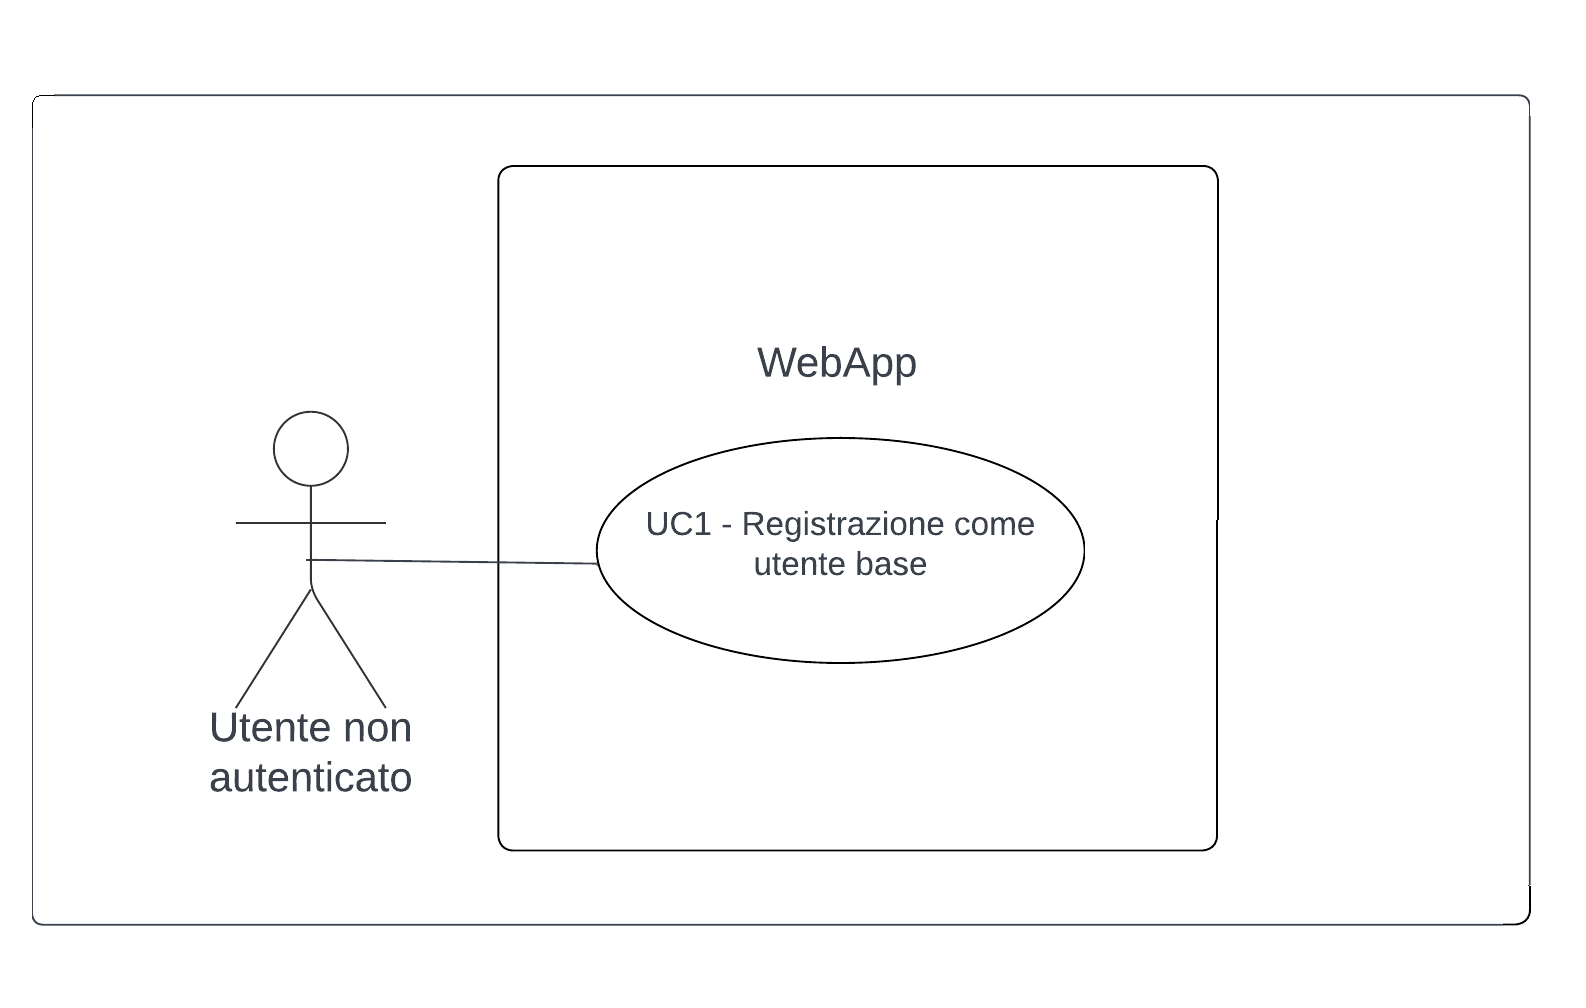
\includegraphics[width=\textwidth]{ucd/UCD1_corretto.png}
\end{figure}
\textbf{Attori principali}: 
\begin{itemize}
    \item Utente non autenticato
\end{itemize}
\textbf{Precondizioni}:
\begin{itemize}
    \item L'utente non è ancora autenticato
\end{itemize}
\textbf{Postcondizioni}: 
\begin{itemize}
    \item L'utente si è registrato ed è riconosciuto come utente base 
\end{itemize}
\textbf{\textit{Trigger}_G}:
\begin{itemize}
    \item L'utente sceglie di registrarsi come utente base
\end{itemize}
\textbf{\textit{Scenario}_G principale}:
\begin{enumerate}
    \item L'utente inserisce le informazioni, ovvero:
    \begin{enumerate}
        \item Nome
        \item Cognome
        \item Email
        \item Password
    \end{enumerate}
    \item L'utente inserisce allergie e intolleranze se presenti
    \item L'utente conferma di volersi registrare con le informazioni fornite
\end{enumerate}
\textbf{Scenari alternativi}:
\begin{itemize}
    \item Inserimento informazioni utente errate: 
    \begin{enumerate}
        \item Campo nome:
        \begin{enumerate}
            \item L'utente lascia il nome vuoto
            \item L'utente usa solo spazi (" ") 
            \item L'utente usa caratteri speciali
            \item L'utente usa caratteri numerici
        \end{enumerate}
        \item Campo cognome:
        \begin{enumerate}
            \item L'utente lascia il cognome vuoto
            \item L'utente usa solo spazi (" ") 
            \item L'utente usa caratteri speciali
            \item L'utente usa caratteri numerici
        \end{enumerate}
        \item Campo email:
        \begin{enumerate}
            \item L'utente lascia il campo email vuoto
            \item L'utente non inserisce una email nel formato: xxxxx@yyy.zz
            \item L'utente inserisce una email già registrata
        \end{enumerate}
        \item Campo password:
        \begin{enumerate}
            \item L'utente lascia il campo password vuoto
            \item L'utente inserisce una password troppo corta (minore di 6 caratteri)
            \item L'utente inserisce una password troppo lunga (maggiore di 24 caratteri)
            \item L'utente inserisce una password senza caratteri minuscoli
            \item L'utente inserisce una password senza caratteri maiuscoli
            \item L'utente inserisce una password senza caratteri numerici
            \item L'utente inserisce una password senza caratteri speciali
        \end{enumerate}
    \end{enumerate}
    \item Viene visualizzato un errore
    \item L'utente decide se annullare o riprovare
\end{itemize}

\begin{comment}    
    1.1.  L'utente lascia il campo nome vuoto
    
    1.2.  L'utente lascia il campo cognome vuoto
    
    1.3a.  L'utente lascia il campo email vuoto
    
    1.3b.  L'utente non inserisce una email nel formato: xxxxx@yyy.zz
    
    1.3c.  L'utente inserisce una email già registrata
    
    1.4a.  L'utente lascia il campo password vuoto
    
    1.4b.  L'utente inserisce una password troppo corta (minore di 6 caratteri)
    
    1.4c.  L'utente inserisce una password troppo lunga (maggiore di 24 caratteri)
    
    1.4d.  L'utente inserisce una password senza caratteri minuscoli
    
    1.4e.  L'utente inserisce una password senza caratteri maiuscoli
    
    1.4f.  L'utente inserisce una password senza caratteri numerici
    
    1.4g.  L'utente inserisce una password senza caratteri speciali

    % 1.5. L'utente lascia il campo allergie e intolleranze vuoto
    
    2.  Viene visualizzato un errore esplicativo
    
    3.  Viene data la possibilità di rifare la registrazione come utente base
    \item L'utente decide di annullare l'operazione di registrazione
\end{comment}
\begin{comment}
\subsubsection{UC1 - Registrazione come utente base}\label{usecase:1}
\textbf{Attori}: 
\begin{itemize}
    \item Utente non autenticato
\end{itemize}
\textbf{Precondizioni}:
\begin{itemize}
    \item L'utente non è ancora autenticato
\end{itemize}
\textbf{Postcondizioni}: 
\begin{itemize}
    \item L'utente si è registrato ed è riconosciuto come utente base 
\end{itemize}
\textbf{\textit{Trigger}_G}:
\begin{itemize}
    \item L'utente sceglie di registrarsi come utente base
\end{itemize}
\textbf{\textit{Scenario}_G principale}:
\begin{enumerate}
    \item L'utente inserisce:
    \begin{enumerate}
        \item Nome
        \item Cognome
        \item Email valida %(\nameref{usecase:1_1})
        \item Passoword che rispetta i criteri indicati %(\nameref{usecase:1_2})
    \end{enumerate}
        \item l'utente \textbf{può} inserire eventuali allergie e intolleranze
\end{enumerate}
\textbf{Scenari secondari}:
\begin{enumerate}
    \item L'utente può decidere di interrompere l'operazione di registrazione in qualsiasi momento
    \item Nel caso in cui l'utente inserisca una mail non valida, oppure inserisca una password non valida, oppure lasci qualche campo obbligatorio vuoto:
    \begin{enumerate}
        \item L'utente non viene registrato presso il sistema
        \item Viene visualizzato un errore esplicativo
        \item Viene data la possibilità di rifare la registrazione come utente base
    \end{enumerate}
\end{enumerate}
\end{comment}


% $\textit{caso d'uso}_G$ UC1.1 - Inserimento credenziali
\subsubsection{UC1.1 - Inserimento email}\label{usecase:1_1}
\textbf{Attori}:
\begin{itemize}
    \item Utente
\end{itemize}
\textbf{Precondizioni}:
\begin{itemize}
    \item L'utente non ha ancora effettuato l'accesso
\end{itemize}
\textbf{Postcondizioni}:
\begin{itemize}
    \item L'utente ha inserito una email valida
\end{itemize}
\textbf{Scenario principale}:
\begin{enumerate}
    \item L'utente inserice un'email univoca
\end{enumerate}
\textbf{Scenari secondari}:
\begin{enumerate}
    \item Nel caso in cui l'email sia già presente all'interno del sistema, l'utente viene notificato attraverso un messaggio visivo.
    \item Viene data la possibilità all'utente di scegliere un'email valida.
\end{enumerate}

%caso d'uso UC1.2 - Inserimento intolleranze
\subsubsection{UC1.2 Inserimento password}\label{usecase:1_2}
\textbf{Attori}:
\begin{itemize}
    \item Utente
\end{itemize}
\textbf{Precondizioni}:
\begin{itemize}
    \item L'utente non ha ancora esegutio l'accesso
\end{itemize}
\textbf{Postcondizioni}:
\begin{itemize}
    \item L'utente ha inserito una password valida
\end{itemize}
\textbf{\textit{Scenario}_G principale}:
\begin{enumerate}
    \item L'utente inserisce una password che rispetta i vincoli imposti.
\end{enumerate}
\textbf{Scenari secondari}:
\begin{enumerate}
    \item Se la password non rispetta i vincoli imposti dal sistema, l'utente viene notificato con un messaggio a schermo.
    \item All'utente viene data la possibilitá di scegliere un'altra password.
\end{enumerate}         

% $\textit{caso d'uso}_G$ UC3 - Inserimento informazioni utente
%\input{uc/uc1_4}

% $\textit{diagramma dei casi d'uso}_G$ UCD2 - $\textit{Prenotazione}_G$ tavolo
\newpage

% $\textit{caso d'uso}_G$ UC2 - Registrazione come amministratore
\subsection{UC2 - Registrazione come amministratore}\label{usecase:2}

\begin{figure}[H]
    \centering
    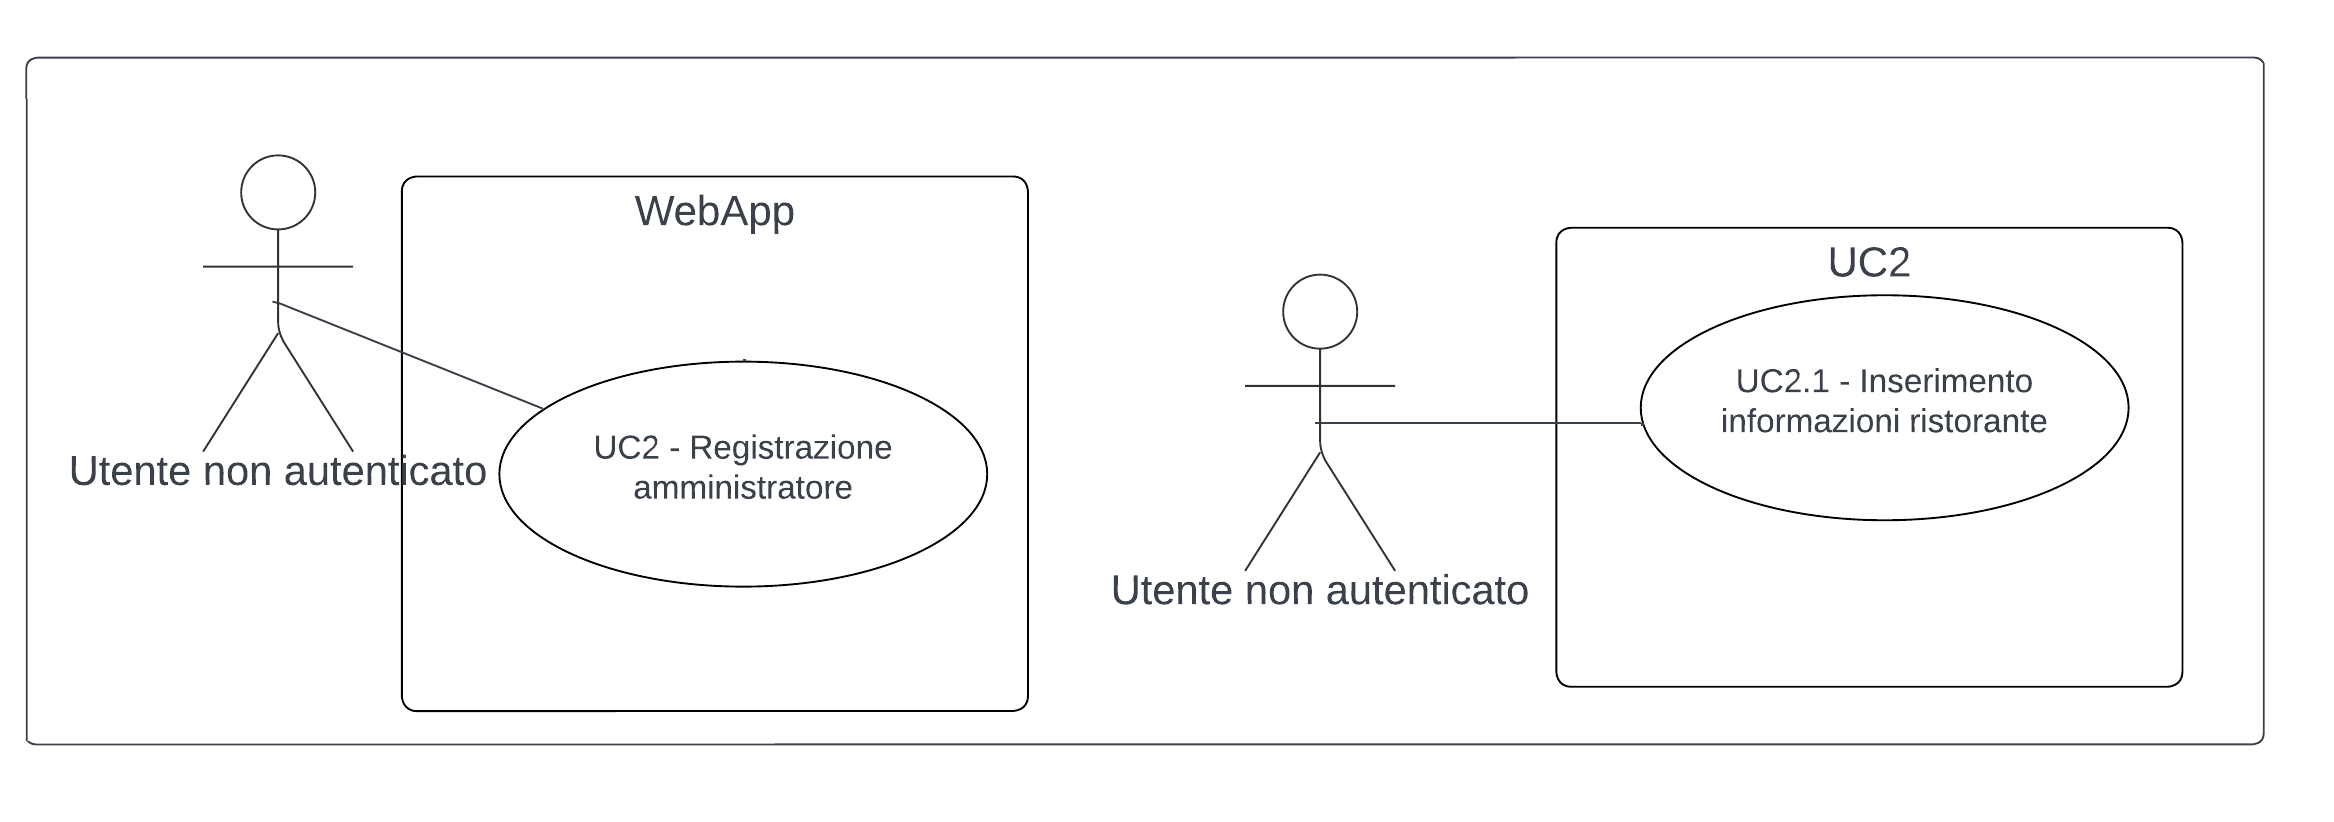
\includegraphics[width=0.9\linewidth]{ucd/UCD2_corretto.png}
\caption{Registrazione come amministratore}
\end{figure}

\textbf{Attori principali}: 
\begin{itemize}
    \item Utente non autenticato.
\end{itemize}
\textbf{Precondizioni}:
\begin{itemize}
    \item L'utente è connesso al $\textit{Sistema}_G$;
    \item L'utente ha ricevuto un link di invito speciale che permette la registrazione come amministratore.
\end{itemize}
\textbf{Postcondizioni}: 
\begin{itemize}
    \item L'utente si è registrato ed è riconosciuto dal $\textit{Sistema}_G$ come amministratore.
\end{itemize}
\textbf{Scenario principale}:
\begin{enumerate}
    \item L'utente inserisce il nome;
    \item L'utente inserisce il cognome;
    \item L'utente inserisce un'email valida;
    \item L'utente inserisce la password che rispetta i criteri indicati;
    \item L'utente inserisce le informazioni del ristorante (\nameref{usecase:2_1}).
\end{enumerate}
\textbf{Scenari alternativi}:
\begin{itemize}
    \item 1.1.  L'utente lascia il campo nome vuoto;
    
    1.2.  L'utente lascia il campo cognome vuoto;
    
    1.3a.  L'utente lascia il campo email vuoto;
    
    1.3b.  L'utente non inserisce una email nel formato: xxxxx@yyy.zz;
    
    1.3c.  L'utente inserisce una email già registrata;
    
    1.4a.  L'utente lascia il campo password vuoto;
    
    1.4b.  L'utente inserisce una password troppo corta (minore di 6 caratteri);
    
    1.4c.  L'utente inserisce una password troppo lunga (maggiore di 24 caratteri);
    
    1.4d.  L'utente inserisce una password senza caratteri minuscoli;
    
    1.4e.  L'utente inserisce una password senza caratteri maiuscoli;
    
    1.4f.  L'utente inserisce una password senza caratteri numerici;
    
    1.4g.  L'utente inserisce una password senza caratteri speciali;

    1.5.  L'utente lascia il campo nome ristorante vuoto;

    1.6.  L'utente lascia il campo città vuoto;
    
    1.7.  L'utente lascia il campo recapiti del ristorante vuoto;
    
    1.8.  L'utente lascia il campo orario apertura vuoto;
    
    1.9.  L'utente lascia il campo coperti disponibili vuoto;
    
    1.10.  L'utente lascia il campo tipologia cucina vuoto;
    
    2.  Viene visualizzato un errore esplicativo;
    
    3.  Viene data la possibilità di rifare la registrazione come amministratore;
    \item L'utente decide di annullare l'operazione di registrazione.
\end{itemize}
\subsubsection{UC2.1 - Inserimento credenziali}\label{usecase:2_1}
\begin{figure}[H]
    \centering
    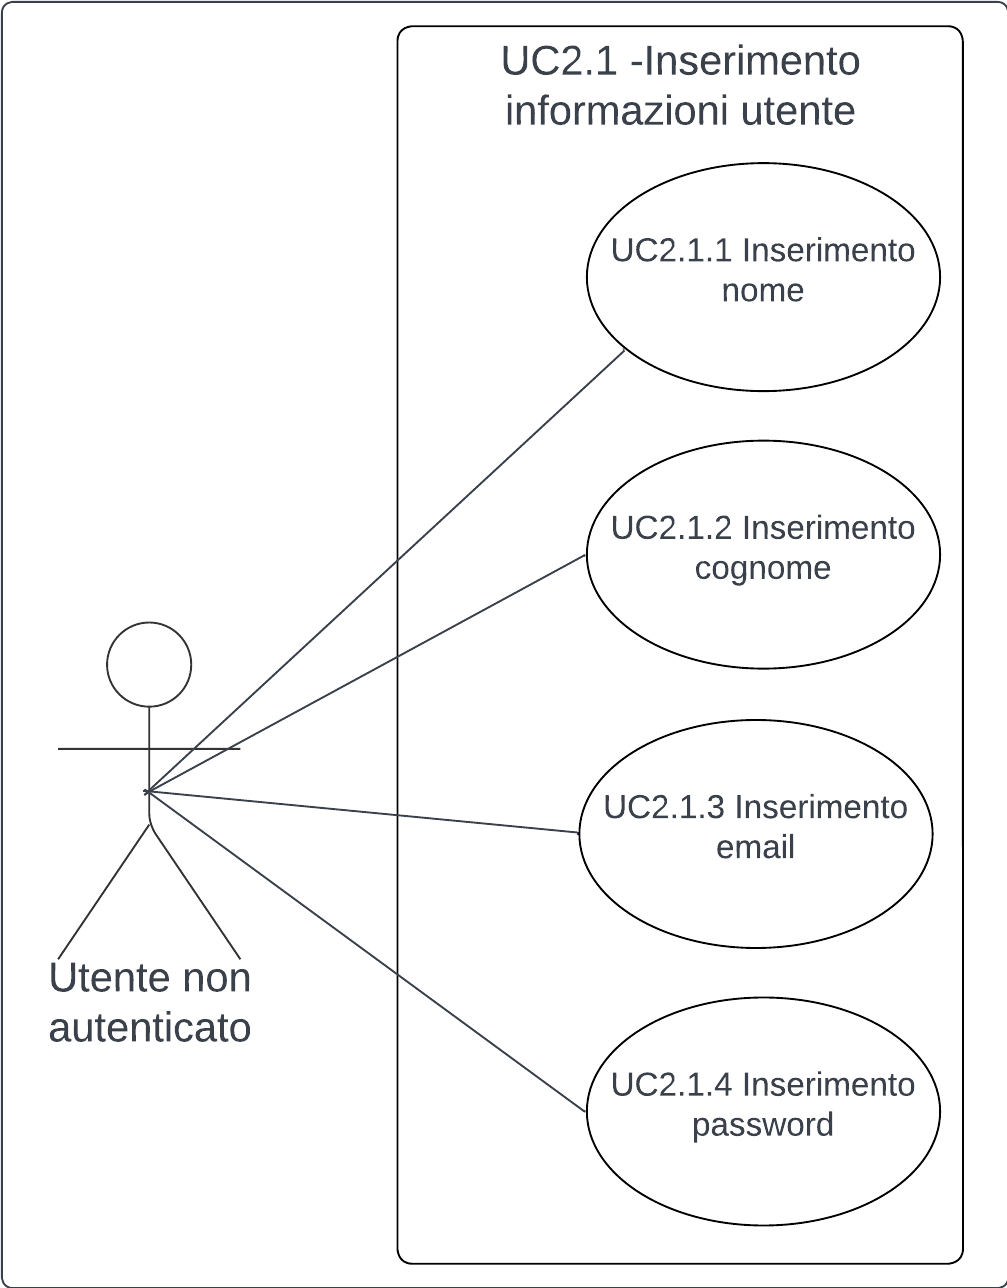
\includegraphics[scale=0.7]{ucd/UCD2.1.png}
\caption{Registrazione come amministratore}
\end{figure}
\textbf{Attori}:
\begin{itemize}
    \item Utente non autenticato
\end{itemize}
\textbf{Precondizioni}:
\begin{itemize}
     \item L'utente è connesso al $\textit{Sistema}_G$;
    \item L'utente ha ricevuto un link di invito speciale che permette la registrazione come amministratore.
\end{itemize}
\textbf{Postcondizioni}:
\begin{itemize}
    \item L'utente ha inserito delle credenziali valide
\end{itemize}
\textbf{Scenario principale}:
\begin{enumerate}
    \item l'utente inserisce le sue informazioni:
    \begin{itemize}
        \item nome (\nameref{usecase:2_1_1})
        \item cognome (\nameref{usecase:2_1_2})
        \item email (\nameref{usecase:2_1_3})
        \item password (\nameref{usecase:2_1_4})
    \end{itemize}
\end{enumerate}

\subsubsection{UC2.1.1 - Inserimento nome}\label{usecase:2_1_1}
\textbf{Attori}:
\begin{itemize}
    \item Utente non autenticato.
\end{itemize}
\textbf{Precondizioni}:
\begin{itemize}
   \item L'utente è connesso al $\textit{Sistema}_G$;
    \item L'utente ha ricevuto un link di invito speciale che permette la registrazione come amministratore.
\end{itemize}
\textbf{Postcondizioni}:
\begin{itemize}
    \item L'utente ha inserito un nome valido all'interno del $\textit{sistema}_G$.
\end{itemize}
\textbf{Scenario principale}:
\begin{enumerate}
    \item l'utente inserisce un nome valido.
\end{enumerate}
\textbf{Scenari secondari}:

\begin{enumerate}
    \item inserimento nome errato:
    \begin{enumerate}
        \item L'utente lascia il nome vuoto;
        \item L'utente usa solo spazi (" ");
        \item L'utente usa caratteri speciali;
        \item L'utente usa caratteri numerici;
    \end{enumerate}

\end{enumerate}


\subsubsection{UC2.1.2 - Inserimento cognome}\label{usecase:2_1_2}
\textbf{Attori}:
\begin{itemize}
    \item Utente non autenticato.
\end{itemize}
\textbf{Precondizioni}:
\begin{itemize}
    \item L'utente è connesso al $\textit{Sistema}_G$;
    \item L'utente ha ricevuto un link di invito speciale che permette la registrazione come amministratore.
\end{itemize}
\textbf{Postcondizioni}:
\begin{itemize}
    \item L'utente ha inserito un cognome valido all'interno del $\textit{sistema}_G$.
\end{itemize}
\textbf{Scenario principale}:
\begin{enumerate}
    \item l'utente inserisce un cognome valido.
\end{enumerate}
\textbf{Scenari secondari}:

\begin{enumerate}
    \item inserimento cognome errato:
    \begin{enumerate}
        \item L'utente lascia il nome vuoto;
        \item L'utente usa solo spazi (" ");
        \item L'utente usa caratteri speciali;
        \item L'utente usa caratteri numerici;
    \end{enumerate}    
\end{enumerate}

\subsubsection{UC2.1.3 - Inserimento email}\label{usecase:2_1_3}
\textbf{Attori}:
\begin{itemize}
    \item Utente non autenticato.
\end{itemize}
\textbf{Precondizioni}:
\begin{itemize}
    \item L'utente è connesso al $\textit{Sistema}_G$;
    \item L'utente ha ricevuto un link di invito speciale che permette la registrazione come amministratore.
\end{itemize}
\textbf{Postcondizioni}:
\begin{itemize}
    \item L'utente ha inserito un'email valida all'interno del $\textit{sistema}_G$.
\end{itemize}
\textbf{Scenario principale}:
\begin{enumerate}
    \item l'utente inserisce un indirizzo email valido.
\end{enumerate}
\textbf{Scenari secondari}:

\begin{enumerate}
    \item inserimento di un indirizzo email errato:
    \begin{enumerate}
            \item L'utente lascia il campo email vuoto;
            \item L'utente non inserisce una email nel formato: xxxxx@yyy.zz;
            \item L'utente inserisce una email già registrata;
        \end{enumerate} 
\end{enumerate}

\subsubsection{UC2.1.4 - Inserimento password}\label{usecase:2_1_4}
\textbf{Attori}:
\begin{itemize}
    \item Utente non autenticato.
\end{itemize}
\textbf{Precondizioni}:
\begin{itemize}
    \item L'utente è connesso al $\textit{Sistema}_G$;
    \item L'utente ha ricevuto un link di invito speciale che permette la registrazione come amministratore.
\end{itemize}
\textbf{Postcondizioni}:
\begin{itemize}
    \item L'utente ha inserito una password valida all'interno del $\textit{sistema}_G$.
\end{itemize}
\textbf{Scenario principale}:
\begin{enumerate}
    \item l'utente inserisce una password valida.
\end{enumerate}
\textbf{Scenari secondari}:

\begin{enumerate}
    \item inserimento di una password errata:
    \begin{enumerate}
            \item L'utente lascia il campo password vuoto;
            \item L'utente inserisce una password troppo corta (minore di 6 caratteri);
            \item L'utente inserisce una password troppo lunga (maggiore di 24 caratteri);
            \item L'utente inserisce una password senza caratteri minuscoli;
            \item L'utente inserisce una password senza caratteri maiuscoli;
            \item L'utente inserisce una password senza caratteri numerici;
            \item L'utente inserisce una password senza caratteri speciali;
        \end{enumerate} 
\end{enumerate}
\subsubsection{UC2.2 - Inserimento informazioni ristorante amministratore}\label{usecase:2_2}

\begin{figure}[H]
    \centering
    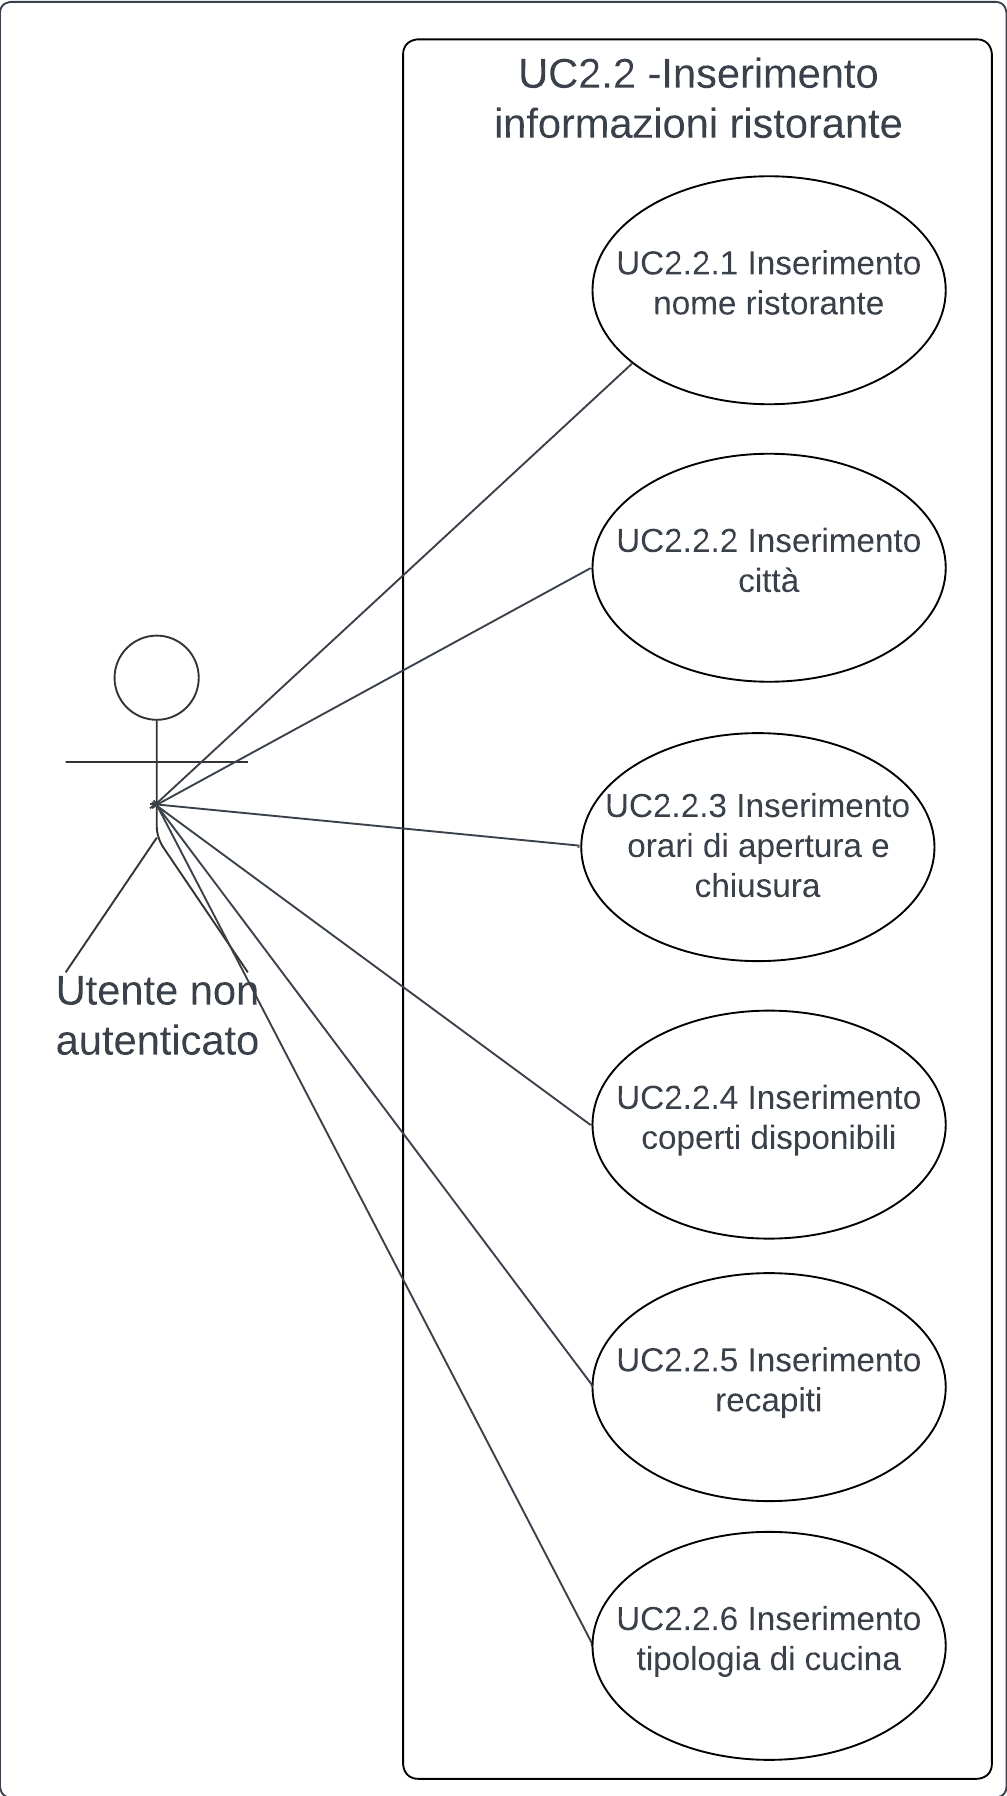
\includegraphics[scale=0.7]{ucd/UCD2.2_finale.png}
\caption{Registrazione come amministratore}
\end{figure}

\textbf{Attori}:
\begin{itemize}
    \item Utente non autenticato.
\end{itemize}
\textbf{Precondizioni}:
\begin{itemize}
    \item L'utente è connesso al $\textit{Sistema}_G$;
    \item L'utente ha ricevuto un link di invito speciale che permette la registrazione come amministratore.
\end{itemize}
\textbf{Postcondizioni}:
\begin{itemize}
    \item L'utente ha inserito le informazioni del ristorante da registrare.
\end{itemize}
\textbf{Scenario principale}:
\begin{enumerate}
    \item L'utente inserisce il nome del ristorante (\nameref{usecase:2_2_1});
    \item L'utente inserisce la città (\nameref{usecase:2_2_2}); 
    \item L'utente inserisce l'orario apertura e chiusura (\nameref{usecase:2_2_3});
    \item L'utente inserisce i coperti disponibili (\nameref{usecase:2_2_4});
    \item L'utente inserisce i recapiti del ristorante (\nameref{usecase:2_2_5});
    \item L'utente inserisce la tipologia di cucina (\nameref{usecase:2_2_6}).
\end{enumerate}
\textbf{Scenari secondari}:
    \begin{enumerate}
        \item L'utente lascia dei campi vuoti;
        \item L'utente inserisce dati non validi.
    \end{enumerate}

\subsubsection{UC2.2.1 - Inserimento nome ristorante}\label{usecase:2_2_1}
\textbf{Attori}:
\begin{itemize}
    \item Utente non autenticato.
\end{itemize}
\textbf{Precondizioni}:
\begin{itemize}
    \item L'utente è connesso al $\textit{Sistema}_G$;
    \item L'utente ha ricevuto un link di invito speciale che permette la registrazione come amministratore.
\end{itemize}
\textbf{Postcondizioni}:
\begin{itemize}
    \item L'utente ha inserito il nome del ristorante
\end{itemize}
\textbf{Scenario principale}:
\begin{enumerate}
    \item L'utente inserisce il nome del ristorante;
\end{enumerate}
\textbf{Scenario secondario}:
\begin{enumerate}
    \item L'utente lascia il nome vuoto;
    \item L'utente usa solo spazi (" ");
    \item L'utente usa caratteri speciali;
\end{enumerate}
\subsubsection{UC2.2.2 - Inserimento città}\label{usecase:2_2_2}
\textbf{Attori}:
\begin{itemize}
    \item Utente non autenticato.
\end{itemize}
\textbf{Precondizioni}:
\begin{itemize}
    \item L'utente è connesso al $\textit{Sistema}_G$;
    \item L'utente ha ricevuto un link di invito speciale che permette la registrazione come amministratore.
\end{itemize}
\textbf{Postcondizioni}:
\begin{itemize}
    \item L'utente ha inserito la città
\end{itemize}
\textbf{Scenario principale}:
\begin{enumerate}
    \item L'utente inserisce il nome della città
\end{enumerate}
\textbf{Scenario secondario}:
\begin{enumerate}
    \item L'utente lascia il campo vuoto;
    \item L'utente usa solo spazi (" ");
    \item L'utente usa caratteri speciali;
\end{enumerate}
\subsubsection{UC2.2.3 - Inserimento orari di apertura e chiusura}\label{usecase:2_2_3}
\textbf{Attori}:
\begin{itemize}
    \item Utente non autenticato.
\end{itemize}
\textbf{Precondizioni}:
\begin{itemize}
    \item L'utente è connesso al $\textit{Sistema}_G$;
    \item L'utente ha ricevuto un link di invito speciale che permette la registrazione come amministratore.
\end{itemize}
\textbf{Postcondizioni}:
\begin{itemize}
    \item L'utente ha gli orari
\end{itemize}
\textbf{Scenario principale}:
\begin{enumerate}
    \item L'utente inserisce l'orario di apertura
    \item L'utente inserisce l'orario di chiusura
\end{enumerate}
\textbf{Scenario secondario}:
\begin{enumerate}
    \item L'utente lascia il campo vuoto;
    \item L'utente inserisce un orario non valido;
\end{enumerate}
\subsubsection{UC2.2.4 - Inserimento coperti disponibili}\label{usecase:2_2_4}
\textbf{Attori}:
\begin{itemize}
    \item Utente non autenticato.
\end{itemize}
\textbf{Precondizioni}:
\begin{itemize}
    \item L'utente è connesso al $\textit{Sistema}_G$;
    \item L'utente ha ricevuto un link di invito speciale che permette la registrazione come amministratore.
\end{itemize}
\textbf{Postcondizioni}:
\begin{itemize}
    \item L'utente ha inserito i coperti
\end{itemize}
\textbf{Scenario principale}:
\begin{enumerate}
    \item L'utente inserisce il numero di coperti
\end{enumerate}
\textbf{Scenario secondario}:
\begin{enumerate}
    \item L'utente lascia il campo vuoto;
    \item L'utente utilizza caratteri diversi dai numeri;
    \item L'utente inserisce un numero non valido (troppo grandi oppure zero)
\end{enumerate}
\subsubsection{UC2.2.5 - Inserimento recapiti}\label{usecase:2_2_5}
\textbf{Attori}:
\begin{itemize}
    \item Utente non autenticato.
\end{itemize}
\textbf{Precondizioni}:
\begin{itemize}
    \item L'utente è connesso al $\textit{Sistema}_G$;
    \item L'utente ha ricevuto un link di invito speciale che permette la registrazione come amministratore.
\end{itemize}
\textbf{Postcondizioni}:
\begin{itemize}
    \item L'utente inserisce i recapiti
\end{itemize}
\textbf{Scenario principale}:
\begin{enumerate}
    \item L'utente inserisce email del ristorante
    \item L'utente inserisce il numero del ristorante
\end{enumerate}
\textbf{Scenario secondario}:
\begin{enumerate}
    \item L'utente lascia i campi vuoti;
    \item L'utente inserisce un numero non valido;
\end{enumerate}
\subsubsection{UC2.2.6 - Inserimento tipologia di cucina}\label{usecase:2_2_6}
\textbf{Attori}:
\begin{itemize}
    \item Utente non autenticato.
\end{itemize}
\textbf{Precondizioni}:
\begin{itemize}
    \item L'utente è connesso al $\textit{Sistema}_G$;
    \item L'utente ha ricevuto un link di invito speciale che permette la registrazione come amministratore.
\end{itemize}
\textbf{Postcondizioni}:
\begin{itemize}
    \item L'utente ha inserito la tipologia di cucina
\end{itemize}
\textbf{Scenario principale}:
\begin{enumerate}
    \item L'utente sceglie la tipologia della cucina del ristorante
\end{enumerate}
\newpage

% $\textit{caso d'uso}_G$ UC4 - Accettazione richiesta prenotazione
%\subsubsection{UC2.2 - Inserimento informazioni ristorante amministratore}\label{usecase:2_2}

\begin{figure}[H]
    \centering
    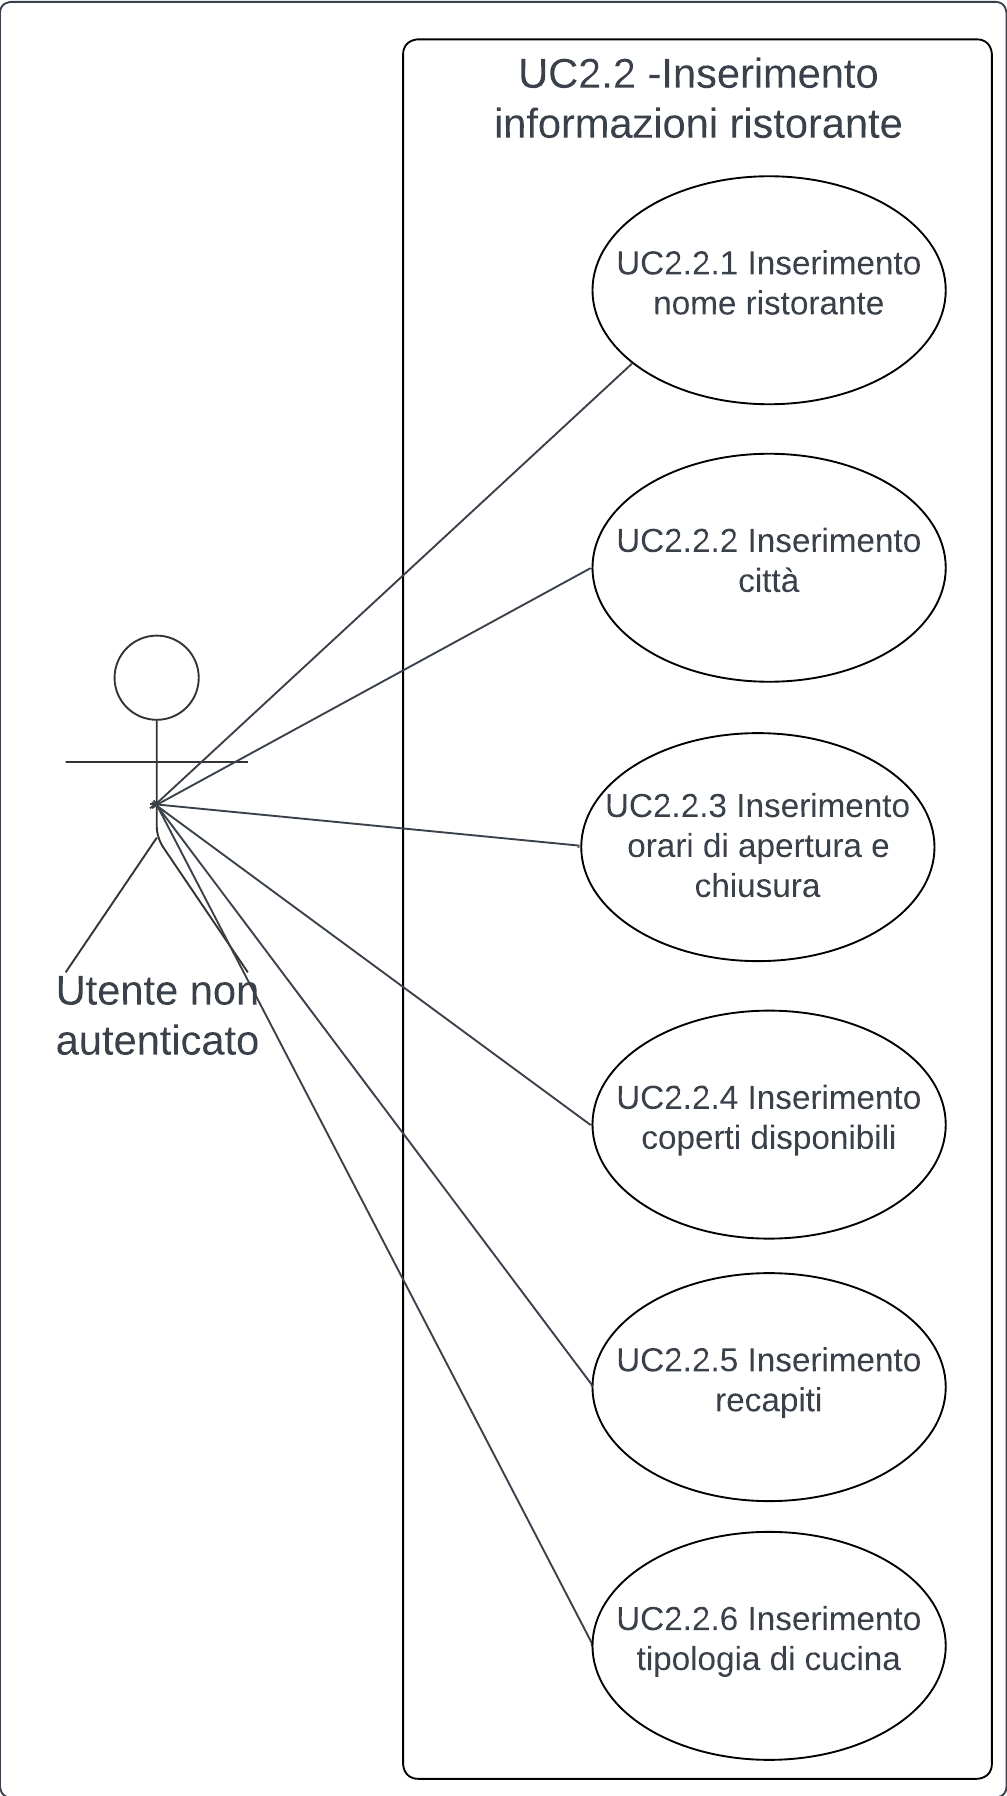
\includegraphics[scale=0.7]{ucd/UCD2.2_finale.png}
\caption{Registrazione come amministratore}
\end{figure}

\textbf{Attori}:
\begin{itemize}
    \item Utente non autenticato.
\end{itemize}
\textbf{Precondizioni}:
\begin{itemize}
    \item L'utente è connesso al $\textit{Sistema}_G$;
    \item L'utente ha ricevuto un link di invito speciale che permette la registrazione come amministratore.
\end{itemize}
\textbf{Postcondizioni}:
\begin{itemize}
    \item L'utente ha inserito le informazioni del ristorante da registrare.
\end{itemize}
\textbf{Scenario principale}:
\begin{enumerate}
    \item L'utente inserisce il nome del ristorante (\nameref{usecase:2_2_1});
    \item L'utente inserisce la città (\nameref{usecase:2_2_2}); 
    \item L'utente inserisce l'orario apertura e chiusura (\nameref{usecase:2_2_3});
    \item L'utente inserisce i coperti disponibili (\nameref{usecase:2_2_4});
    \item L'utente inserisce i recapiti del ristorante (\nameref{usecase:2_2_5});
    \item L'utente inserisce la tipologia di cucina (\nameref{usecase:2_2_6}).
\end{enumerate}
\textbf{Scenari secondari}:
    \begin{enumerate}
        \item L'utente lascia dei campi vuoti;
        \item L'utente inserisce dati non validi.
    \end{enumerate}

\subsubsection{UC2.2.1 - Inserimento nome ristorante}\label{usecase:2_2_1}
\textbf{Attori}:
\begin{itemize}
    \item Utente non autenticato.
\end{itemize}
\textbf{Precondizioni}:
\begin{itemize}
    \item L'utente è connesso al $\textit{Sistema}_G$;
    \item L'utente ha ricevuto un link di invito speciale che permette la registrazione come amministratore.
\end{itemize}
\textbf{Postcondizioni}:
\begin{itemize}
    \item L'utente ha inserito il nome del ristorante
\end{itemize}
\textbf{Scenario principale}:
\begin{enumerate}
    \item L'utente inserisce il nome del ristorante;
\end{enumerate}
\textbf{Scenario secondario}:
\begin{enumerate}
    \item L'utente lascia il nome vuoto;
    \item L'utente usa solo spazi (" ");
    \item L'utente usa caratteri speciali;
\end{enumerate}
\subsubsection{UC2.2.2 - Inserimento città}\label{usecase:2_2_2}
\textbf{Attori}:
\begin{itemize}
    \item Utente non autenticato.
\end{itemize}
\textbf{Precondizioni}:
\begin{itemize}
    \item L'utente è connesso al $\textit{Sistema}_G$;
    \item L'utente ha ricevuto un link di invito speciale che permette la registrazione come amministratore.
\end{itemize}
\textbf{Postcondizioni}:
\begin{itemize}
    \item L'utente ha inserito la città
\end{itemize}
\textbf{Scenario principale}:
\begin{enumerate}
    \item L'utente inserisce il nome della città
\end{enumerate}
\textbf{Scenario secondario}:
\begin{enumerate}
    \item L'utente lascia il campo vuoto;
    \item L'utente usa solo spazi (" ");
    \item L'utente usa caratteri speciali;
\end{enumerate}
\subsubsection{UC2.2.3 - Inserimento orari di apertura e chiusura}\label{usecase:2_2_3}
\textbf{Attori}:
\begin{itemize}
    \item Utente non autenticato.
\end{itemize}
\textbf{Precondizioni}:
\begin{itemize}
    \item L'utente è connesso al $\textit{Sistema}_G$;
    \item L'utente ha ricevuto un link di invito speciale che permette la registrazione come amministratore.
\end{itemize}
\textbf{Postcondizioni}:
\begin{itemize}
    \item L'utente ha gli orari
\end{itemize}
\textbf{Scenario principale}:
\begin{enumerate}
    \item L'utente inserisce l'orario di apertura
    \item L'utente inserisce l'orario di chiusura
\end{enumerate}
\textbf{Scenario secondario}:
\begin{enumerate}
    \item L'utente lascia il campo vuoto;
    \item L'utente inserisce un orario non valido;
\end{enumerate}
\subsubsection{UC2.2.4 - Inserimento coperti disponibili}\label{usecase:2_2_4}
\textbf{Attori}:
\begin{itemize}
    \item Utente non autenticato.
\end{itemize}
\textbf{Precondizioni}:
\begin{itemize}
    \item L'utente è connesso al $\textit{Sistema}_G$;
    \item L'utente ha ricevuto un link di invito speciale che permette la registrazione come amministratore.
\end{itemize}
\textbf{Postcondizioni}:
\begin{itemize}
    \item L'utente ha inserito i coperti
\end{itemize}
\textbf{Scenario principale}:
\begin{enumerate}
    \item L'utente inserisce il numero di coperti
\end{enumerate}
\textbf{Scenario secondario}:
\begin{enumerate}
    \item L'utente lascia il campo vuoto;
    \item L'utente utilizza caratteri diversi dai numeri;
    \item L'utente inserisce un numero non valido (troppo grandi oppure zero)
\end{enumerate}
\subsubsection{UC2.2.5 - Inserimento recapiti}\label{usecase:2_2_5}
\textbf{Attori}:
\begin{itemize}
    \item Utente non autenticato.
\end{itemize}
\textbf{Precondizioni}:
\begin{itemize}
    \item L'utente è connesso al $\textit{Sistema}_G$;
    \item L'utente ha ricevuto un link di invito speciale che permette la registrazione come amministratore.
\end{itemize}
\textbf{Postcondizioni}:
\begin{itemize}
    \item L'utente inserisce i recapiti
\end{itemize}
\textbf{Scenario principale}:
\begin{enumerate}
    \item L'utente inserisce email del ristorante
    \item L'utente inserisce il numero del ristorante
\end{enumerate}
\textbf{Scenario secondario}:
\begin{enumerate}
    \item L'utente lascia i campi vuoti;
    \item L'utente inserisce un numero non valido;
\end{enumerate}
\subsubsection{UC2.2.6 - Inserimento tipologia di cucina}\label{usecase:2_2_6}
\textbf{Attori}:
\begin{itemize}
    \item Utente non autenticato.
\end{itemize}
\textbf{Precondizioni}:
\begin{itemize}
    \item L'utente è connesso al $\textit{Sistema}_G$;
    \item L'utente ha ricevuto un link di invito speciale che permette la registrazione come amministratore.
\end{itemize}
\textbf{Postcondizioni}:
\begin{itemize}
    \item L'utente ha inserito la tipologia di cucina
\end{itemize}
\textbf{Scenario principale}:
\begin{enumerate}
    \item L'utente sceglie la tipologia della cucina del ristorante
\end{enumerate}
\newpage

% $\textit{caso d'uso}_G$ UC5 - Rifiuto richiesta prenotazione
%\input{uc/uc2_3}

%caso d'uso UC2.1 - Ricerca ristorante
%\subsubsection{UC2.1 - Inserimento credenziali}\label{usecase:2_1}
\begin{figure}[H]
    \centering
    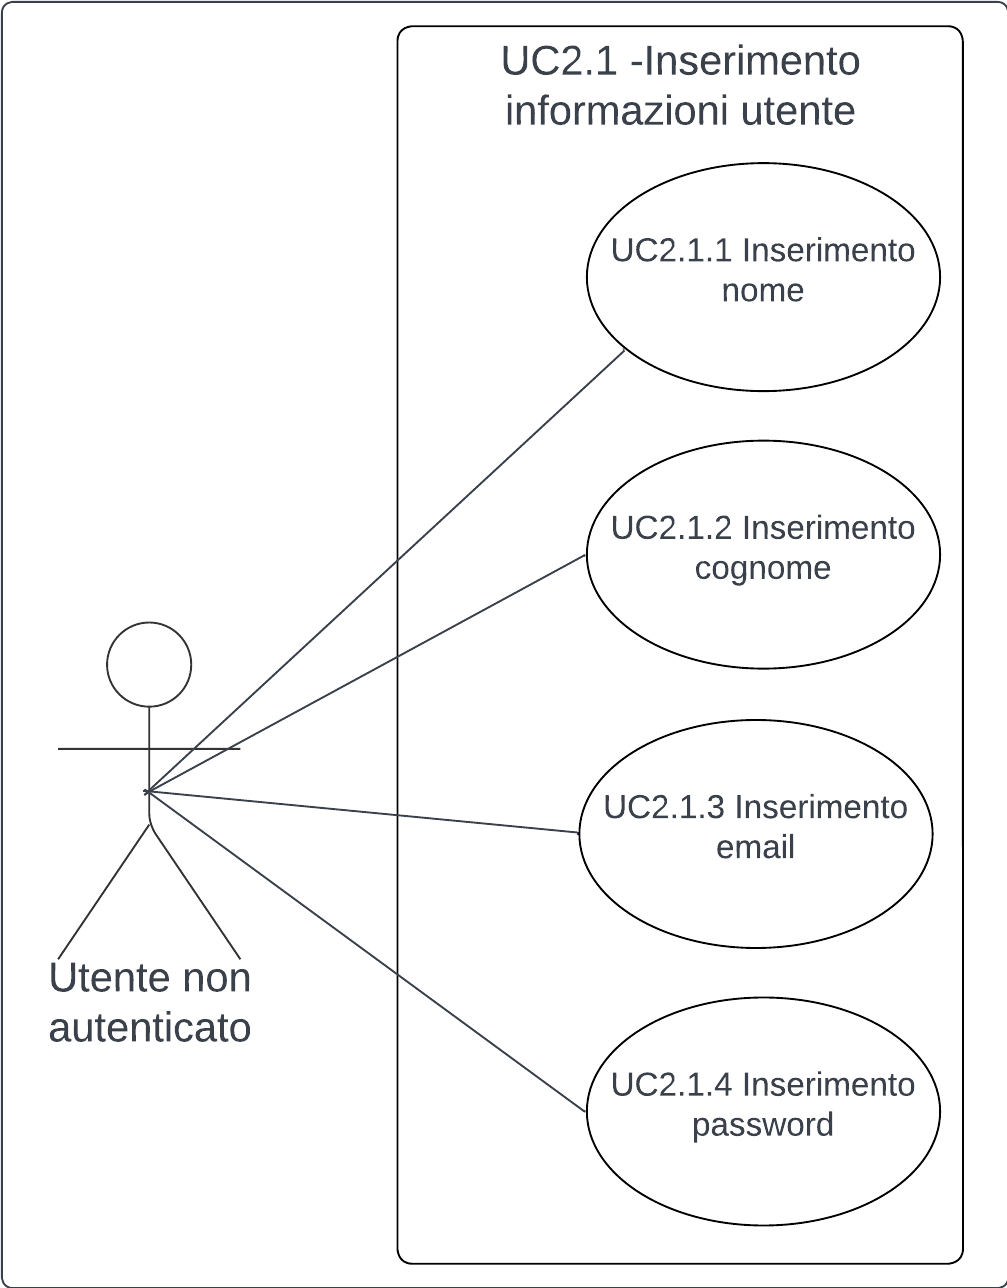
\includegraphics[scale=0.7]{ucd/UCD2.1.png}
\caption{Registrazione come amministratore}
\end{figure}
\textbf{Attori}:
\begin{itemize}
    \item Utente non autenticato
\end{itemize}
\textbf{Precondizioni}:
\begin{itemize}
     \item L'utente è connesso al $\textit{Sistema}_G$;
    \item L'utente ha ricevuto un link di invito speciale che permette la registrazione come amministratore.
\end{itemize}
\textbf{Postcondizioni}:
\begin{itemize}
    \item L'utente ha inserito delle credenziali valide
\end{itemize}
\textbf{Scenario principale}:
\begin{enumerate}
    \item l'utente inserisce le sue informazioni:
    \begin{itemize}
        \item nome (\nameref{usecase:2_1_1})
        \item cognome (\nameref{usecase:2_1_2})
        \item email (\nameref{usecase:2_1_3})
        \item password (\nameref{usecase:2_1_4})
    \end{itemize}
\end{enumerate}

\subsubsection{UC2.1.1 - Inserimento nome}\label{usecase:2_1_1}
\textbf{Attori}:
\begin{itemize}
    \item Utente non autenticato.
\end{itemize}
\textbf{Precondizioni}:
\begin{itemize}
   \item L'utente è connesso al $\textit{Sistema}_G$;
    \item L'utente ha ricevuto un link di invito speciale che permette la registrazione come amministratore.
\end{itemize}
\textbf{Postcondizioni}:
\begin{itemize}
    \item L'utente ha inserito un nome valido all'interno del $\textit{sistema}_G$.
\end{itemize}
\textbf{Scenario principale}:
\begin{enumerate}
    \item l'utente inserisce un nome valido.
\end{enumerate}
\textbf{Scenari secondari}:

\begin{enumerate}
    \item inserimento nome errato:
    \begin{enumerate}
        \item L'utente lascia il nome vuoto;
        \item L'utente usa solo spazi (" ");
        \item L'utente usa caratteri speciali;
        \item L'utente usa caratteri numerici;
    \end{enumerate}

\end{enumerate}


\subsubsection{UC2.1.2 - Inserimento cognome}\label{usecase:2_1_2}
\textbf{Attori}:
\begin{itemize}
    \item Utente non autenticato.
\end{itemize}
\textbf{Precondizioni}:
\begin{itemize}
    \item L'utente è connesso al $\textit{Sistema}_G$;
    \item L'utente ha ricevuto un link di invito speciale che permette la registrazione come amministratore.
\end{itemize}
\textbf{Postcondizioni}:
\begin{itemize}
    \item L'utente ha inserito un cognome valido all'interno del $\textit{sistema}_G$.
\end{itemize}
\textbf{Scenario principale}:
\begin{enumerate}
    \item l'utente inserisce un cognome valido.
\end{enumerate}
\textbf{Scenari secondari}:

\begin{enumerate}
    \item inserimento cognome errato:
    \begin{enumerate}
        \item L'utente lascia il nome vuoto;
        \item L'utente usa solo spazi (" ");
        \item L'utente usa caratteri speciali;
        \item L'utente usa caratteri numerici;
    \end{enumerate}    
\end{enumerate}

\subsubsection{UC2.1.3 - Inserimento email}\label{usecase:2_1_3}
\textbf{Attori}:
\begin{itemize}
    \item Utente non autenticato.
\end{itemize}
\textbf{Precondizioni}:
\begin{itemize}
    \item L'utente è connesso al $\textit{Sistema}_G$;
    \item L'utente ha ricevuto un link di invito speciale che permette la registrazione come amministratore.
\end{itemize}
\textbf{Postcondizioni}:
\begin{itemize}
    \item L'utente ha inserito un'email valida all'interno del $\textit{sistema}_G$.
\end{itemize}
\textbf{Scenario principale}:
\begin{enumerate}
    \item l'utente inserisce un indirizzo email valido.
\end{enumerate}
\textbf{Scenari secondari}:

\begin{enumerate}
    \item inserimento di un indirizzo email errato:
    \begin{enumerate}
            \item L'utente lascia il campo email vuoto;
            \item L'utente non inserisce una email nel formato: xxxxx@yyy.zz;
            \item L'utente inserisce una email già registrata;
        \end{enumerate} 
\end{enumerate}

\subsubsection{UC2.1.4 - Inserimento password}\label{usecase:2_1_4}
\textbf{Attori}:
\begin{itemize}
    \item Utente non autenticato.
\end{itemize}
\textbf{Precondizioni}:
\begin{itemize}
    \item L'utente è connesso al $\textit{Sistema}_G$;
    \item L'utente ha ricevuto un link di invito speciale che permette la registrazione come amministratore.
\end{itemize}
\textbf{Postcondizioni}:
\begin{itemize}
    \item L'utente ha inserito una password valida all'interno del $\textit{sistema}_G$.
\end{itemize}
\textbf{Scenario principale}:
\begin{enumerate}
    \item l'utente inserisce una password valida.
\end{enumerate}
\textbf{Scenari secondari}:

\begin{enumerate}
    \item inserimento di una password errata:
    \begin{enumerate}
            \item L'utente lascia il campo password vuoto;
            \item L'utente inserisce una password troppo corta (minore di 6 caratteri);
            \item L'utente inserisce una password troppo lunga (maggiore di 24 caratteri);
            \item L'utente inserisce una password senza caratteri minuscoli;
            \item L'utente inserisce una password senza caratteri maiuscoli;
            \item L'utente inserisce una password senza caratteri numerici;
            \item L'utente inserisce una password senza caratteri speciali;
        \end{enumerate} 
\end{enumerate}

% $\textit{caso d'uso}_G$ UC3 - $\textit{Ordinazione}_G$ collaborativa
\subsection{UC3 - Ordinazione collaborativa}\label{usecase:3}

\begin{figure}[H]
    \centering
    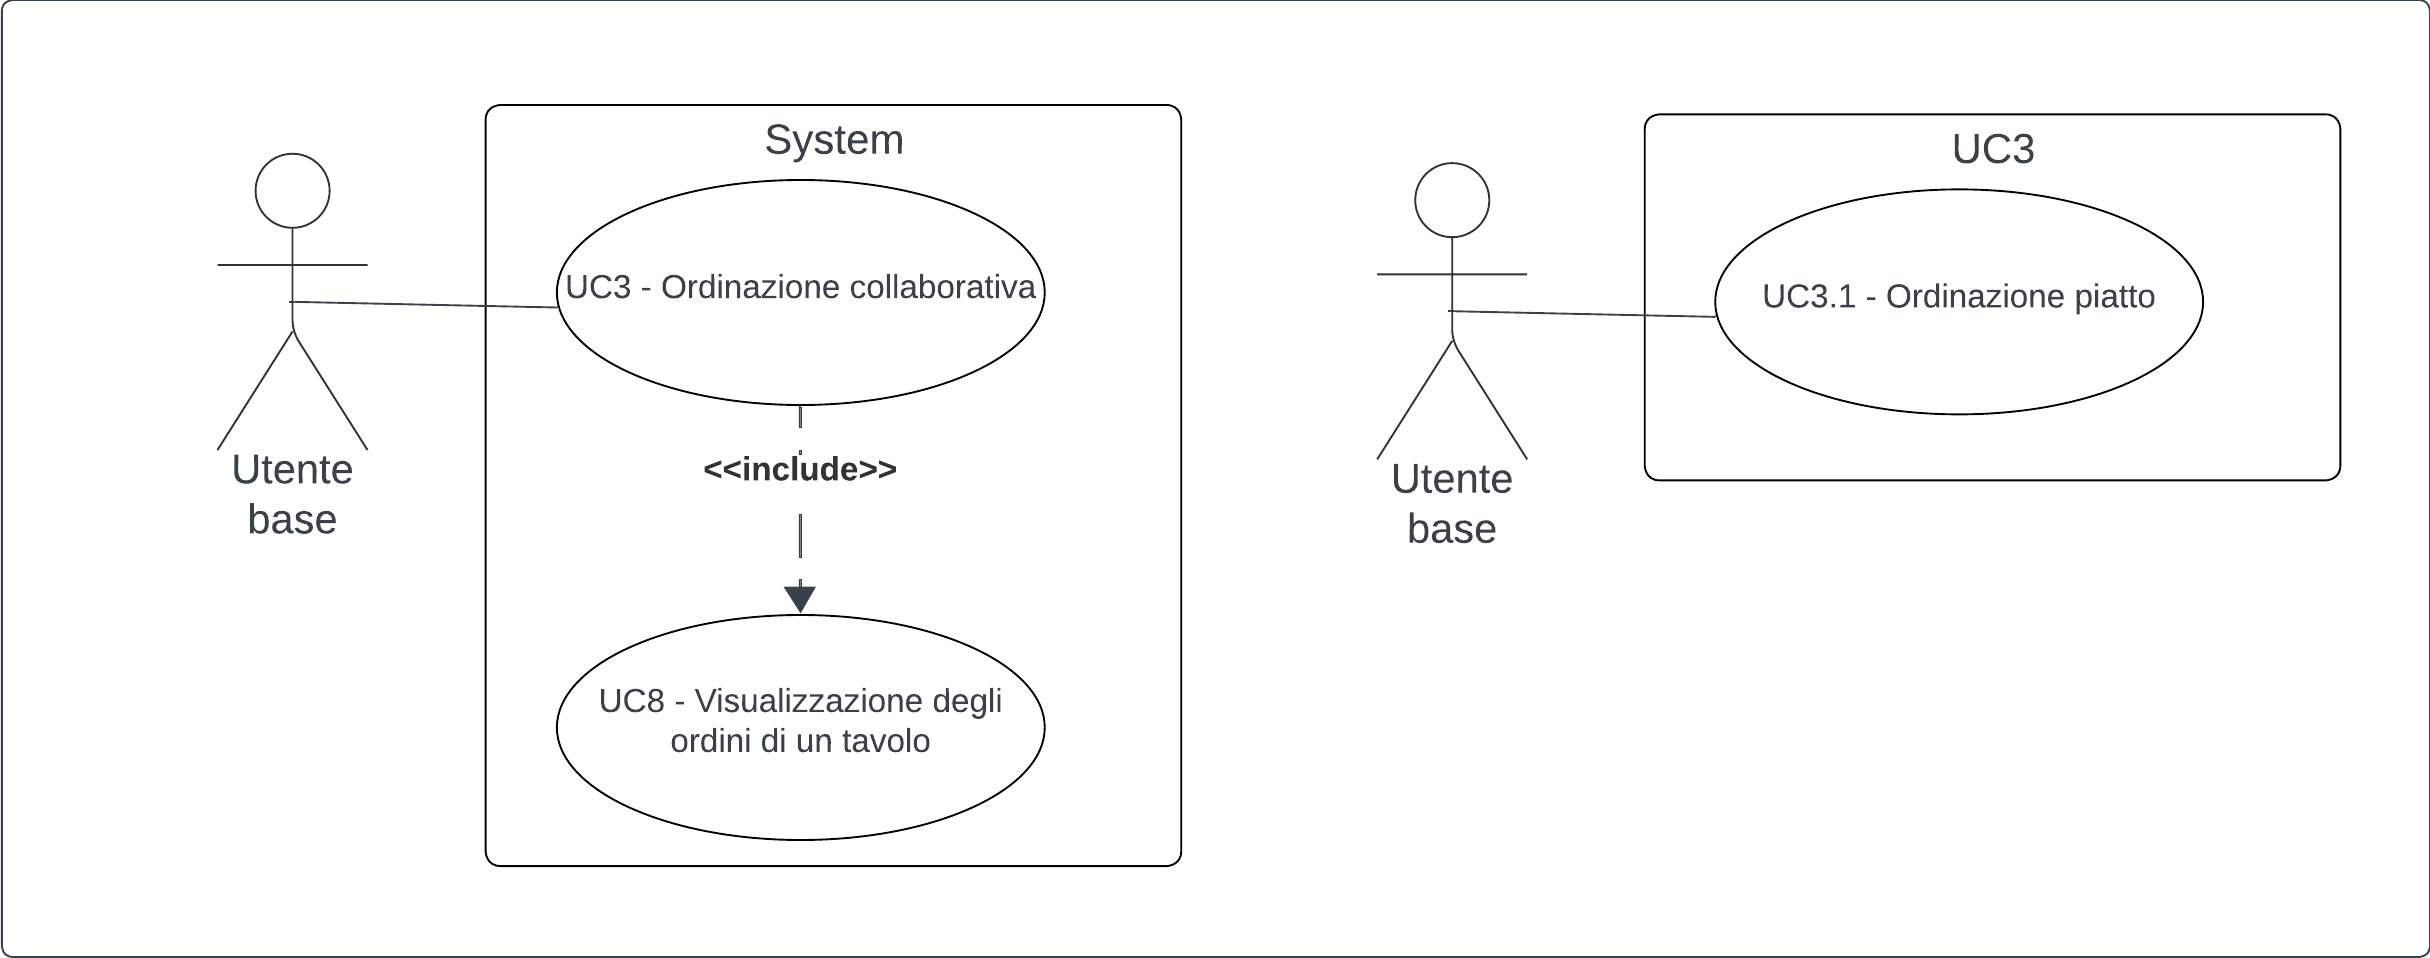
\includegraphics[width=0.9\linewidth]{ucd/UCD3_nuovo.png}
\end{figure}

\textbf{Attori}:
\begin{itemize}
    \item Utente base
\end{itemize}
\textbf{Precondizioni}:
\begin{itemize}
    \item L'utente è autenticato dal sistema 
    \item L'utente ha prenotato un tavolo (\nameref{usecase:23})
    \item La prenotazione associata all'ordinazione è stata accettata dall'utente amministratore del ristorante (\nameref{usecase:19})
    \item Il limite di tempo per l'ordinazione non è ancora scaduto
\end{itemize}
\textbf{Postcondizioni}:
\begin{itemize}
    \item L'utente ha confermato la propria ordinazione delle pietanze associata ad una prenotazione.
\end{itemize}
\textbf{\textit{Scenario}_G principale}:
\begin{enumerate}
    \item L'utente crea il proprio ordine:
    \begin{itemize}
    \item L'utente sceglie il pasto da ordinare (\nameref{usecase:3_1}); nel caso in cui la pietanza ordinata contenga allergeni segnalati dall'utente in fase di registrazione, deve essere notificato prima di  aggiungere la pietanza all'ordine.
    \item L'utente può scegliere di: modificare la quantità degli ingredienti; rimuoverne alcuni ingredienti; aggiungere degli ingredienti (\nameref{usecase:3_1}).
    \end{itemize}
    \item L'utente visualizza il riepilogo del suo ordine e quelli degli altri utenti con cui ha prenotato il tavolo (\nameref{usecase:8}).
    \item L'utente conferma l'ordinazione.
    \item Il sistema notifica il ristorante mediante \textit{push-notification}.
\end{enumerate}


\subsubsection{UC3.1 - Ordinazione piatto}\label{usecase:3_1}

\textbf{Attori}:
\begin{itemize}
    \item Utente base autenticato
\end{itemize}
\textbf{Precondizioni}:
\begin{itemize}
    \item L'utente è autenticato dal sistema 
    \item L'utente ha prenotato un tavolo (\nameref{usecase:23})
    \item La prenotazione associata all'ordinazione è stata accettata dall'utente amministratore del ristorante (\nameref{usecase:19})
    \item Il limite di tempo per l'ordinazione non è ancora scaduto
\end{itemize}
\textbf{Postcondizioni}:
\begin{itemize}
    \item L'utente ha ordinato il piatto
\end{itemize}
\textbf{\textit{Trigger}_G}:
\begin{itemize}
    \item L'utente vuole aggiungere un piatto alla ordinazione collaborativa
\end{itemize}
\textbf{\textit{Scenario}_G principale}:
\begin{enumerate}
    \item L'utente sceglie tra la lista delle pietanze una che vuole aggiungere al proprio ordine
    \item L'utente sceglie la quantità della pietanza
    \item Di ogni pietanza:
    \begin{itemize}
        \item L'utente visualizza gli ingredienti
        \item L'utente può aggiungere ingredienti
        \item L'utente può rimuovere ingredienti
    \end{itemize}
    \item L'utente conferma il piatto
\end{enumerate}
\newpage

\begin{comment}
\subsection{UC3 - Ordinazione collaborativa}\label{usecase:3}

\begin{figure}[H]
    \centering
    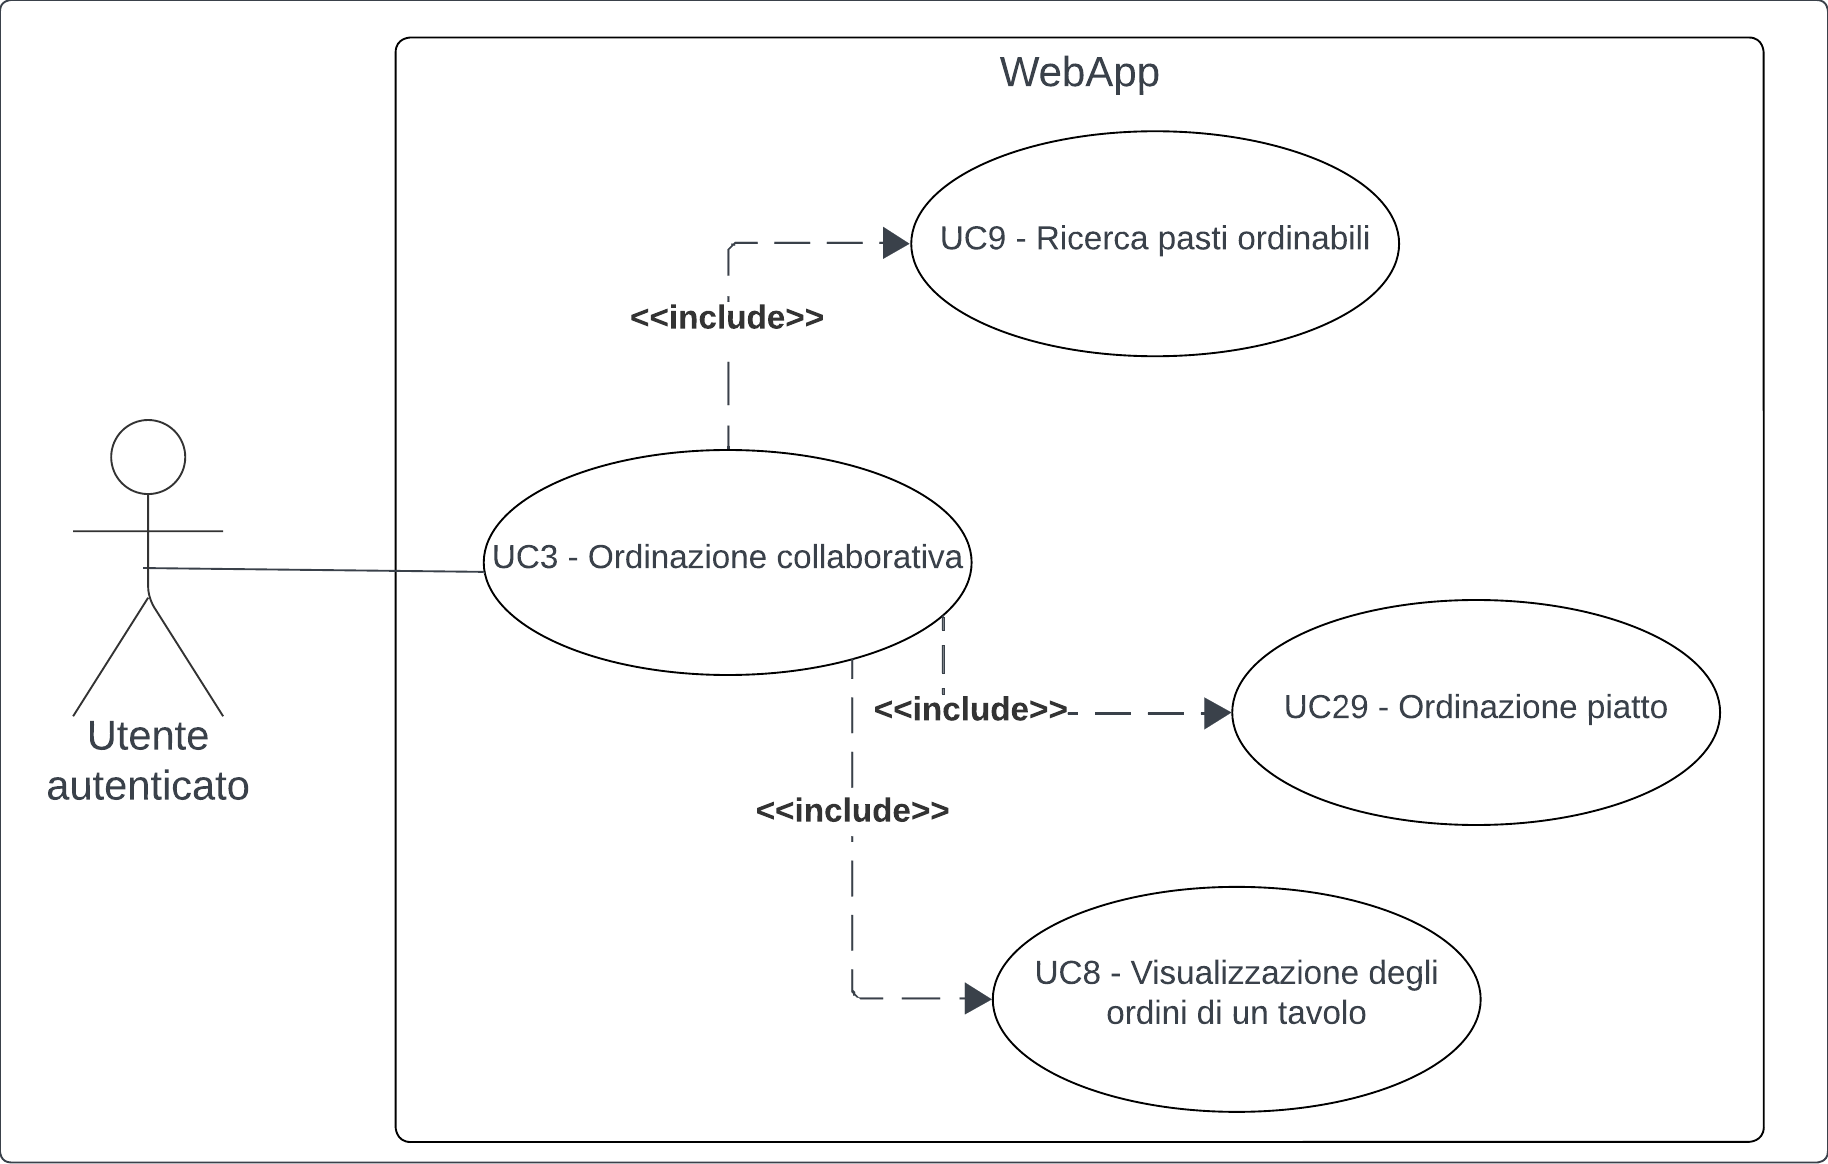
\includegraphics[width=0.9\linewidth]{ucd/UCD3.png}
\end{figure}

\textbf{Attori}:
\begin{itemize}
    \item Utente base autenticato
\end{itemize}
\textbf{Precondizioni}:
\begin{itemize}
    \item L'utente è autenticato dal sistema 
    \item L'utente ha prenotato un tavolo (\nameref{usecase:23})
    \item La prenotazione associata all'ordinazione è stata accettata dall'utente amministratore del ristorante (\nameref{usecase:19})
    \item Il tempo per l'ordinazione non è scaduto
\end{itemize}
\textbf{Postcondizioni}:
\begin{itemize}
    \item L'utente ha confermato l'ordinazione delle pietanze associata ad una prenotazione.
\end{itemize}
\textbf{\textit{Scenario}_G principale}:
\begin{enumerate}
    \item L'utente ricerca i pasti ordinabili (\nameref{usecase:9})
    \item L'utente sceglie il pasto da ordinare (\nameref{usecase:29}); nel caso in cui la pietanza ordinata contenga allergeni segnalati dall'utente in fase di registrazione, deve essere notificato prima di  aggiungere la pietanza all'ordine.
    \item L'utente può scegliere di: modificare la quantità degli ingredienti; rimuoverne alcuni ingredienti; aggiungere degli ingredienti (\nameref{usecase:29}).
    \item L'utente visualizza il riepilogo del suo ordine e quelli degli altri utenti con cui ha prenotato il tavolo (\nameref{usecase:8}).
    \item L'utente conferma l'ordinazione.
    \item Il sistema notifica il ristorante mediante \textit{push-notification}.
\end{enumerate}
\newpage
\end{comment}

% $\textit{caso d'uso}_G$ UC4 - Interazione con lo staff
\subsection{UC4 - Chat con l'Utente base}\label{usecase:4}
%diagramma dei casi d'uso 4
\begin{figure}[H]
  \centering
  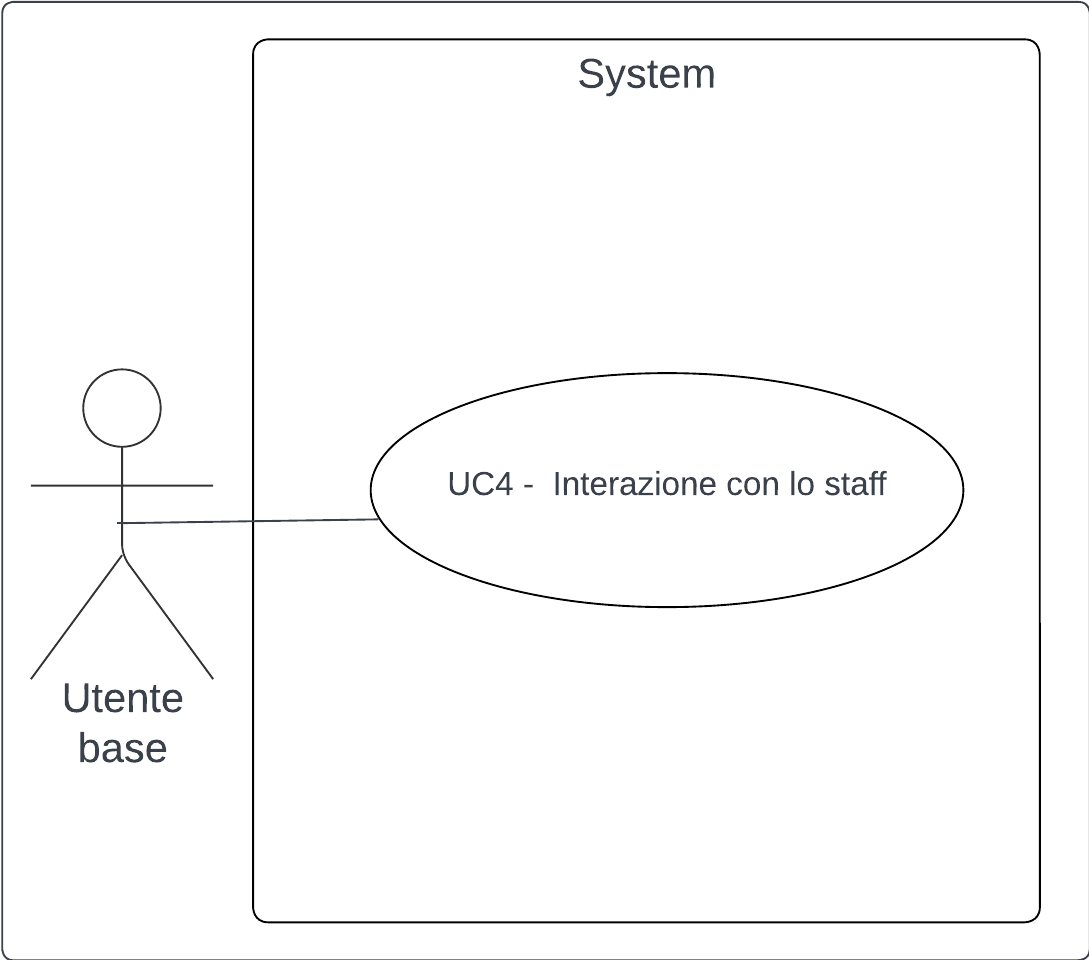
\includegraphics[width=0.5\textwidth]{ucd/UCD4.png}
  \caption{Interazione con lo staff}
\end{figure}
\textbf{Attori}:
\begin{itemize}
    \item Utente base.
\end{itemize}
\textbf{Precondizioni}:
\begin{itemize}
    \item L'utente è connesso al $\textit{Sistema}_G$.
\end{itemize}
\textbf{Postcondizioni}:
\begin{itemize}
    \item L'utente ha comunicato con l'amministratore del ristorante.
\end{itemize}
\textbf{Scenario principale}:
\begin{enumerate}
    \item L'utente seleziona un ristorante con cui comunicare;
    \item Il $\textit{sistema}_G$ crea una chat bidirezionale;
    \item L'utente può comunicare con l'amministratore:
    \begin{itemize}
        \item L'utente può scrivere del testo e inviarlo;
        \item L'utente visualizza l'eventuale risposta;
    \end{itemize}
    \item Durante la comunicazione verranno scambiati messaggi tramite notifica (\textit{push-notification});
    \item L'utente riceve una notifica (push-notification), mostrando:
    \begin{enumerate}
        \item Il nome del ristorante;
        \item Il nome dell'amministratore;
        \item La preview del messaggio.
    \end{enumerate}
\end{enumerate}
\textbf{Scenari alternativi}:
\begin{enumerate}
    \item L'utente non inserisce un messaggio valido:
    \begin{enumerate}
        \item Lascia il campo vuoto;
        \item Immette del testo non valido;
        \item Il testo è troppo lungo;
    \end{enumerate}
    \item L'utente visualizza l'errore e il messaggio non può venire inviato.
\end{enumerate}
\newpage
%\subsubsection{UC4.1 - Chat bidirezionale con l'amministratore}\label{usecase:4_1}
\textbf{Attori}:
\begin{itemize}
    \item Utente base
\end{itemize}
\textbf{Precondizioni}:
\begin{itemize}
    \item L'utente è autenticato dal sistema
    \item L'utente ha selezionato un ristorante
\end{itemize}
\textbf{Postcondizioni}:
\begin{itemize}
    \item L'utente ha comunicato con l'amministratore del ristorante
\end{itemize}
\textbf{Scenari principali}:
\begin{enumerate}
    \item Il sistema crea una chat biderezionale
    \item L'utente può scrivere del testo e inviarlo
    \item L'utente visualizza l'eventuale risposta
\end{enumerate}
\textbf{Scenari alternativi}:
\begin{enumerate}
    \item L'utente non inserisce un messaggio valido:
    \begin{enumerate}
        \item Lascia il campo vuoto
        \item Immette del testo non valido
        \item Il testo è troppo lungo
    \end{enumerate}
    \item L'utente visualizza l'errore e il messaggio non può venire inviato
\end{enumerate}
%\subsubsection{UC4.1 - Chat bidirezionale con l'amministratore}\label{usecase:4_1}
\textbf{Attori}:
\begin{itemize}
    \item Utente base
\end{itemize}
\textbf{Precondizioni}:
\begin{itemize}
    \item L'utente è autenticato dal sistema
    \item L'utente ha selezionato un ristorante
\end{itemize}
\textbf{Postcondizioni}:
\begin{itemize}
    \item L'utente ha comunicato con l'amministratore del ristorante
\end{itemize}
\textbf{Scenari principali}:
\begin{enumerate}
    \item Il sistema crea una chat biderezionale
    \item L'utente può scrivere del testo e inviarlo
    \item L'utente visualizza l'eventuale risposta
\end{enumerate}
\textbf{Scenari alternativi}:
\begin{enumerate}
    \item L'utente non inserisce un messaggio valido:
    \begin{enumerate}
        \item Lascia il campo vuoto
        \item Immette del testo non valido
        \item Il testo è troppo lungo
    \end{enumerate}
    \item L'utente visualizza l'errore e il messaggio non può venire inviato
\end{enumerate}

% $\textit{caso d'uso}_G$ UC5 - Divisione del conto
\subsection{UC5 - Pagamento conto}\label{usecase:5}
\begin{figure}[H]
    \centering
    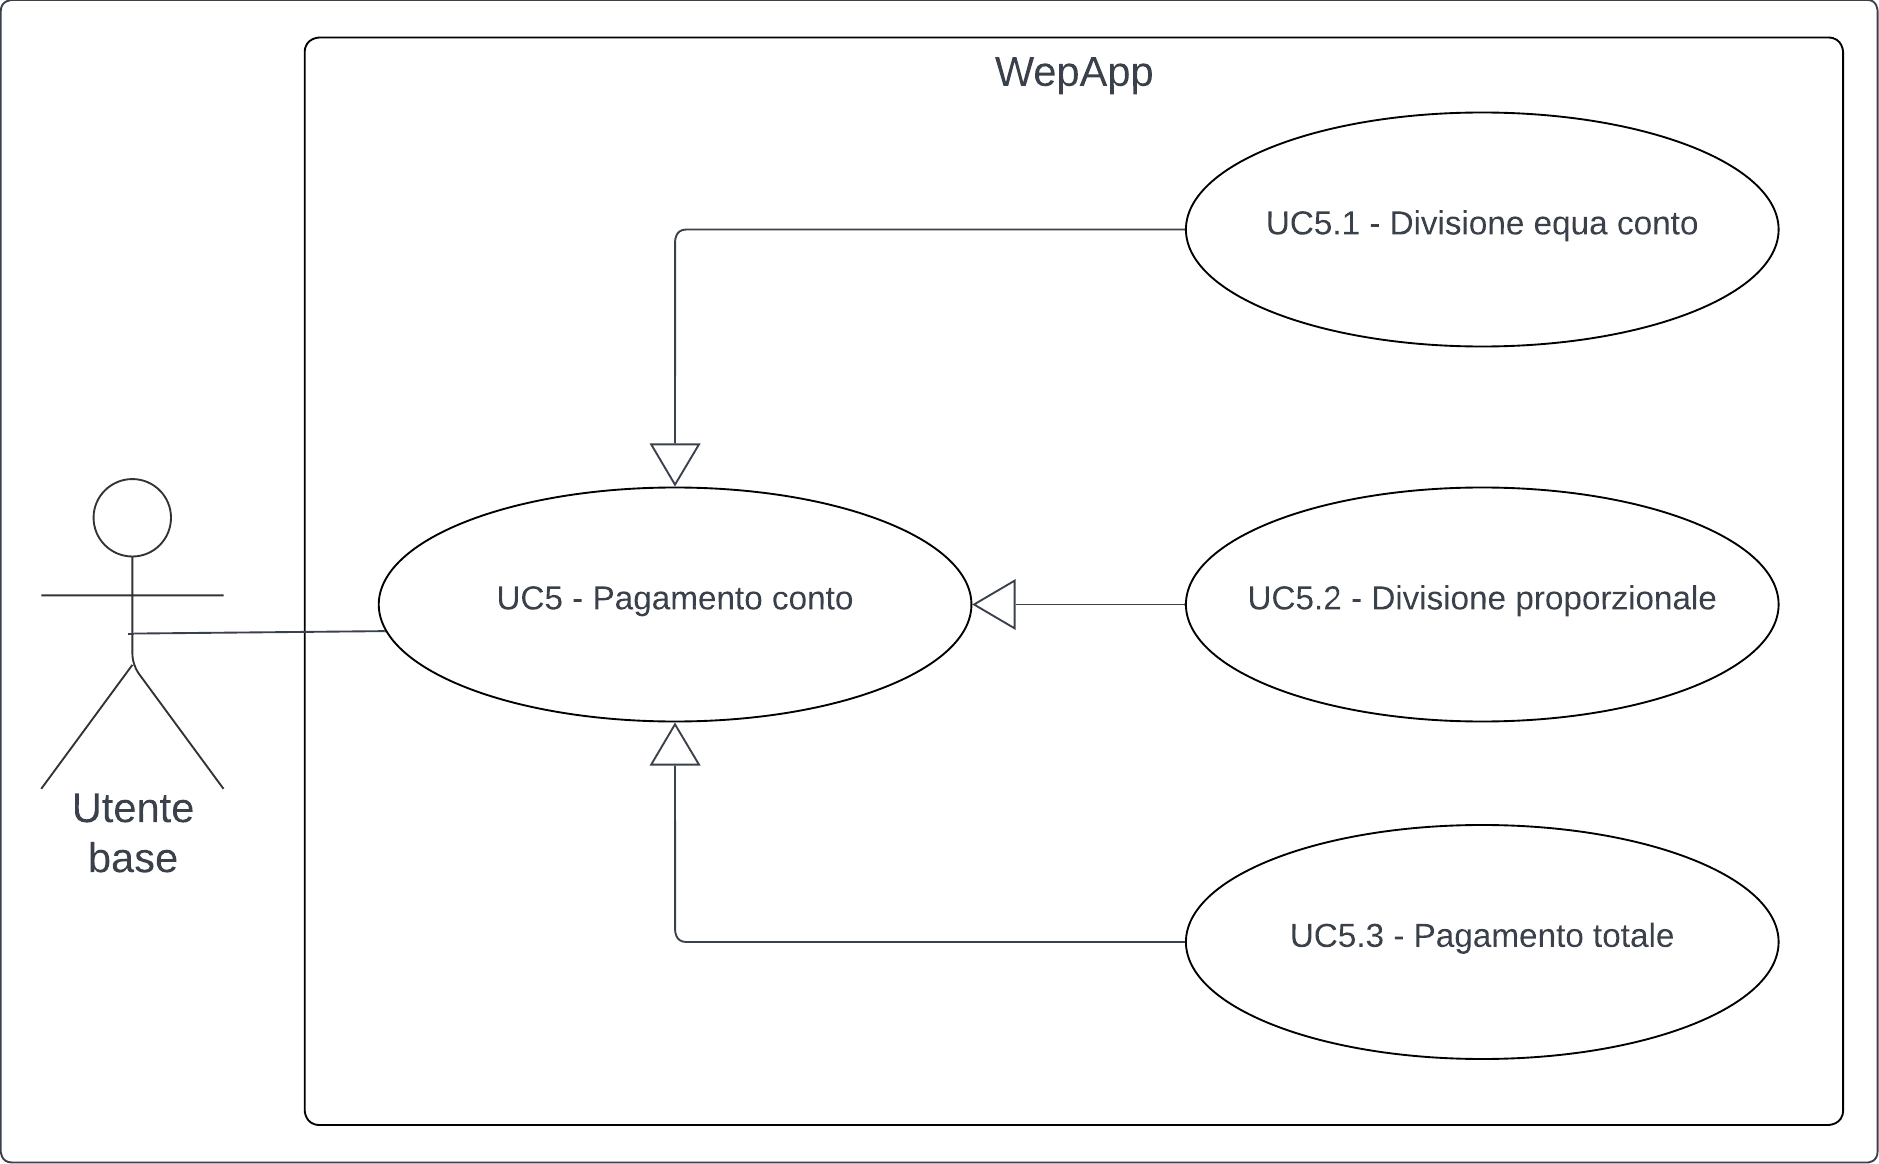
\includegraphics[width=0.7\textwidth]{ucd/UCD5.png}
\end{figure}
\textbf{Attori}:
\begin{itemize}
    \item Utente base autenticato
\end{itemize}
\textbf{Precondizioni}:
\begin{itemize}
    \item L'utente deve aver prenotato un tavolo
    \item L'utente deve aver ordinato (\nameref{usecase:3})
\end{itemize}
\textbf{\textit{Postcondizione}_G}:
\begin{itemize}
    \item Il conto del tavolo è stato pagato
\end{itemize}
\textbf{Scenari principali}:
\begin{enumerate}
    \item L'utente può selezionare tra:
    \begin{enumerate}
        \item divisione equa
        \item proporzionale
        \item pagamento totale
    \end{enumerate}
    \item Ogni utente può decidere se pagare solo la sua parte oppure anche le parti di altri utenti
    \item L'amministratore riceve aggiornamenti riguardanti allo stato del conto del tavolo tramite notifiche (push-notification)
\end{enumerate}
\subsubsection{UC5.1 - Divisione equa}\label{usecase:5.1}
\textbf{Attori}:
\begin{itemize}
    \item Utente base autenticato
\end{itemize}
\textbf{Precondizioni}:
\begin{itemize}
    \item L'utente deve aver prenotato un tavolo
    \item L'utente deve aver ordinato (\nameref{usecase:3})
    \item L'utente che ha creato l'ordinazione collaborativa deve aver scelto questo pagamento
\end{itemize}
\textbf{\textit{Postcondizione}_G}:
\begin{itemize}
    \item Il conto del tavolo è stato pagato
\end{itemize}
\textbf{Scenari principali}:
\begin{enumerate}
    \item L'utente paga la sua parte del conto
\end{enumerate}
\subsubsection{UC5.2 - Divisione proporzionale}\label{usecase:5.2}
\textbf{Attori}:
\begin{itemize}
    \item Utente base autenticato
\end{itemize}
\textbf{Precondizioni}:
\begin{itemize}
    \item L'utente deve aver prenotato un tavolo
    \item L'utente deve aver ordinato (\nameref{usecase:3})
    \item L'utente che ha creato l'ordinazione collaborativa deve aver scelto questo pagamento
\end{itemize}
\textbf{Postcondizione}:
\begin{itemize}
    \item Il conto del tavolo è stato pagato
\end{itemize}
\textbf{Scenari principali}:
\begin{enumerate}
    \item L'utente paga la sua parte del conto
\end{enumerate}
\subsubsection{UC5.3 - Pagamento totale}\label{usecase:5.3}
\textbf{Attori}:
\begin{itemize}
    \item Utente base.
\end{itemize}
\textbf{Precondizioni}:
\begin{itemize}
    \item L'utente è connesso al $\textit{Sistema}_G$;
    \item L'utente deve aver ordinato (\nameref{usecase:3});
    \item Il conto del tavolo non è ancora stato pagato parzialmente.
\end{itemize}
\textbf{Postcondizione}:
\begin{itemize}
    \item Il conto del tavolo è stato pagato.
\end{itemize}
\textbf{Scenari principali}:
\begin{enumerate}
    \item L'utente paga per tutto il tavolo.
\end{enumerate}
\newpage

% $\textit{caso d'uso}_G$ UC6 - Consultazione delle prenotazioni da parte dell'amministratore
\subsection{UC6 - Consultazione di una prenotazione da parte dell'amministratore}\label{usecase:6}
\begin{figure}[H]
  \centering
  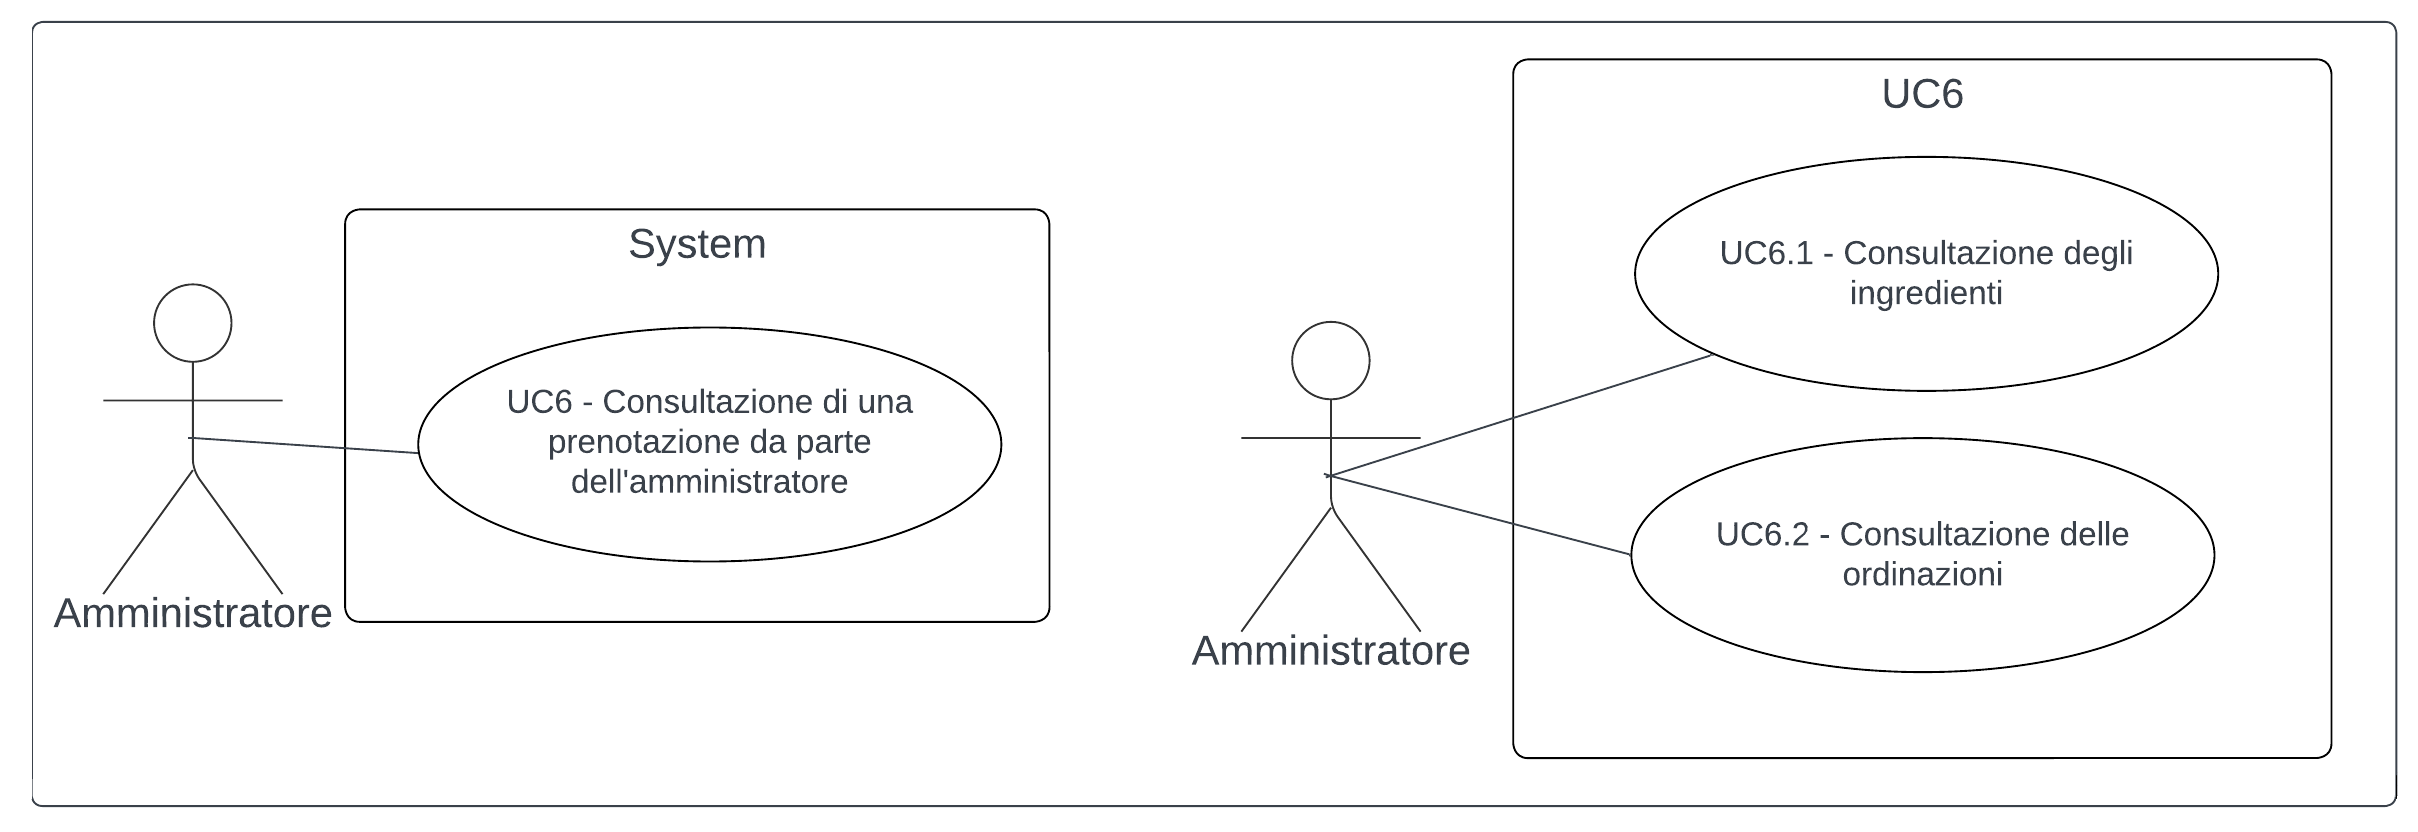
\includegraphics[width=1\textwidth]{ucd/UCD6_new.png}
\end{figure}
\textbf{Attori}:
\begin{itemize}
    \item Amministratore
\end{itemize}
\textbf{Precondizioni}:
\begin{itemize}
    \item L'amministratore in fase di registrazione ha inserito un ristorante di cui poter consultare le prenotazioni
    \item L'amministratore visualizza le prenotazioni dalla lista delle prenotazioni (\nameref{usecase:15})
\end{itemize}
\textbf{Postcondizioni}:
\begin{itemize}
    \item L'amministratore visualizza nel dettaglio le informazioni di una prenotazione
\end{itemize}
\textbf{Scenario principale}:
\begin{enumerate}
    \item L'utente visualizza le informazioni di una singola $\textit{prenotazione}_G$ effettuata, tra cui:
    \begin{enumerate}
        \item gli ingredienti necessari per quella $\textit{prenotazione}_G$ (\nameref{usecase:6_1})
        \item le ordinazioni associate a quella prenotazione
        (\nameref{usecase:6_2})
    \end{enumerate}
\end{enumerate}

%caso d'uso UC6.1 - Consultazione degli ingredienti
\subsubsection{UC6.1 - Consultazione degli ingredienti}\label{usecase:6_1}
\textbf{Attori}:
\begin{itemize}
    \item \textit{Amministratore}_G
\end{itemize}
\textbf{\textit{Precondizione}_G}:
\begin{itemize}
    \item L'amministratore in fase di registrazione ha inserito un ristorante di cui poter consultare le prenotazioni
    \item L'amministratore visualizza le prenotazioni dalla lista delle prenotazioni (\nameref{usecase:15})
\end{itemize}
\textbf{\textit{Postcondizione}_G}:
\begin{itemize}
    \item L'amministratore ha visualizzato la lista di ingredienti necessari per quella prenotazione
\end{itemize}
\textbf{\textit{Scenario}_G principale}:
\begin{enumerate}
    \item L'utente visualizza gli ingredienti necessari per quella ordinazioni inseriti in una lista, per ogni ingrediente si visualizza:
    \begin{enumerate}
        \item Nome
        \item Quantità
    \end{enumerate}
\end{enumerate}

%caso d'uso UC6.2 - Consultazione delle ordinazioni
\subsubsection{UC6.2 - Consultazione delle ordinazioni}\label{usecase:6_2}
\textbf{Attori}:
\begin{itemize}
    \item Amministratore
\end{itemize}
\textbf{Precondizione}:
\begin{itemize}
    \item L'amministratore in fase di registrazione ha inserito un ristorante di cui poter consultare le prenotazioni
    \item L'amministratore visualizza le prenotazioni dalla lista delle prenotazioni (\nameref{usecase:15})
\end{itemize}
\textbf{Postcondizione}:
\begin{itemize}
    \item L'amministratore ha visualizzato le ordinazioni e il loro stato presenti all'interno di una prenotazione
\end{itemize}
\textbf{Scenario principale}:
\begin{enumerate}
    \item L'utente visualizza la lista delle ordinazioni e il loro stato (quanti utenti hanno già ordinato), per ogni ordinazione si visualizza:
    \begin{enumerate}
        \item Piatto
        \item Quantità
    \end{enumerate}
\end{enumerate}
\newpage

% $\textit{caso d'uso}_G$ UC7 - Inserimento di $\textit{feedback}_G$ e recensioni
\subsection{UC7 - Inserimento recensione}\label{usecase:7}
\begin{figure}[H]
  \centering
  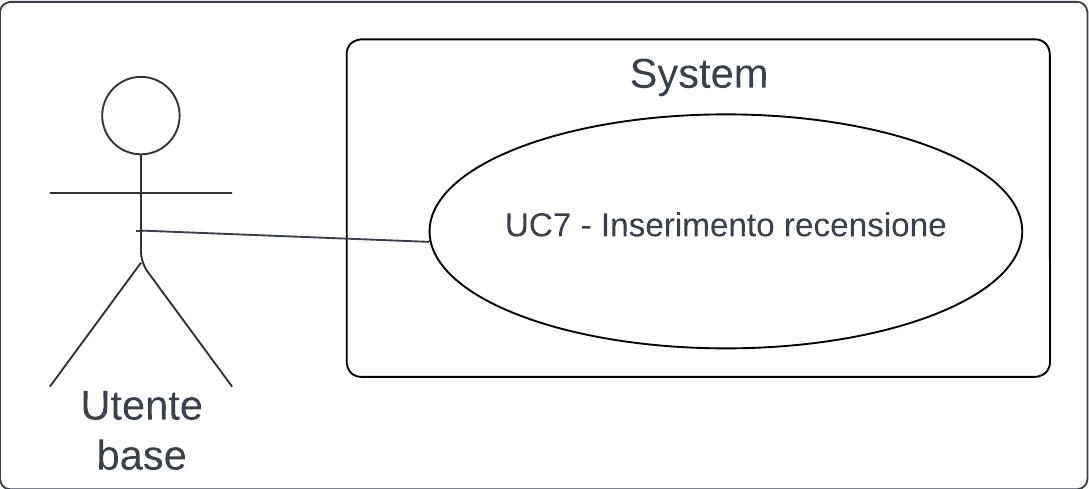
\includegraphics[width=0.7\textwidth]{ucd/UCD7.png}
  \caption{Inserimento recensione}
\end{figure}
\textbf{Attori}:
\begin{itemize}
    \item Utente base.
\end{itemize}
\textbf{Precodizioni}:
\begin{itemize}
    \item L'utente ha scelto di lasciare una recensione.
\end{itemize}
\textbf{Postcondizioni}:
\begin{itemize}
    \item L'utente rilascia una recensione al ristorante selezionato.
\end{itemize}
\textbf{Scenario principale}:
\begin{enumerate}
    \item L'utente selezione un ristorante a cui lasciare una recensione;
    \item L'utente rilascia la recensione sotto forma di numero di stelle su 5 disponibili e con aggiunta di testo;
    \item L'utente conferma la sua recensione.
\end{enumerate}
\textbf{Scenari alternativi}:
\begin{enumerate}
    \item Se la recensione è:
    \begin{enumerate}
        \item Troppo lunga;
        \item Vuota;
    \end{enumerate}
    \item Visualizza un errore;
    \item L'utente deve aggiornare la recensione in modo tale che rispetta i criteri per poterla pubblicare.
\end{enumerate}
\newpage

% $\textit{caso d'uso}_G$ UC8 - Visualizzazione degli ordini di un tavolo
\subsection{UC8 - Visualizzazioni ordini tavolo (utente)}\label{usecase:8}
\begin{figure}[H]
    \centering
    \includegraphics[width=0.9\linewidth]{ucd/ucd8.png}
\end{figure}
\textbf{Attori}:
\begin{itemize}
    \item Utente base
\end{itemize}
\textbf{Precondizioni}:
\begin{itemize}
    \item L'utente è autenticato dal sistema
    \item L'utente ha effettuato un $\textit{ordinazione}_G$ (\nameref{usecase:3})
\end{itemize}
\textbf{Postcondizioni}:
\begin{itemize}
    \item L'utente visualizza il riepilogo dell'ordine includendo anche le pietanze scelte dagli altri utenti
\end{itemize}
\textbf{Scenario principale}:
\begin{enumerate}
    \item L'utente trova la lista delle ordinazioni relative al tavolo
    \item Per ogni ordine visualizza i dettagli (\nameref{usecase:8_1})
\end{enumerate}
\subsubsection{UC8.1 - Visualizzazione dettagli ordine}\label{usecase:8_1}
\textbf{Attori}:
\begin{itemize}
    \item Utente base
\end{itemize}
\textbf{Precondizioni}:
\begin{itemize}
    \item L'utente è autenticato dal sistema
    \item L'utente ha prenotato un tavolo
\end{itemize}
\textbf{Postcondizioni}:
\begin{itemize}
    \item L'utente visualizza i dettagli dell'ordine
\end{itemize}
\textbf{Scenario principale}:
\begin{enumerate}
    \item L'utente visualizza i dettagli dell'ordine, ovvero:
    \begin{enumerate}
        \item Pasto ordinato
        \item Quantità ordinata
        \item La persona che ha effettuato l'ordine
    \end{enumerate}
\end{enumerate}
\newpage

% $\textit{caso d'uso}_G$ UC9 - Ricerca pasti ordinabili
\subsection{UC9 - Modifica del proprio ordine}\label{usecase:9}
\begin{figure}[H]
    \centering
    \includegraphics[width=0.7\linewidth]{ucd/ucd9.png}
\caption{Modifica del proprio ordine}
\end{figure}
\textbf{Attori}:
\begin{itemize}
    \item Utente base.
\end{itemize}
\textbf{Precondizioni}:
\begin{itemize}
    \item L'utente è connesso al $\textit{Sistema}_G$;
    \item L'utente ha creato la propria $\textit{ordinazione}_G$ in precedenza (\nameref{usecase:3});
    \item Il tempo per l'$\textit{ordinazione}_G$ non è scaduto.
\end{itemize}
\textbf{Postcondizioni}:
\begin{itemize}
    \item L'utente ha modificato il proprio ordine e il $\textit{sistema}_G$ aggiorna le informazioni di conseguenza.
\end{itemize}
\textbf{Scenario principale}:
\begin{enumerate}
    \item L'utente può compiere le seguenti azioni per gestire il proprio ordine:
    \begin{enumerate}
        \item Inserire un piatto nell'ordine scegliendo tra la lista delle pietanze;
        \item Scelto un piatto inserito nell'ordine si può:
        \begin{enumerate}
            \item Rimuovere ingredienti;
            \item Aggiungere ingredienti;
            \item Modificare la quantità della pietanza, incluso rimuoverla.
        \end{enumerate}
    \end{enumerate}
\end{enumerate}

\newpage

%caso d'uso UC10 - Rimozione della recensione rilasciata
\subsection{UC10 - Rimozione della recensione rilasciata} \label{usecase:10}
\begin{figure}[H]
    \centering
    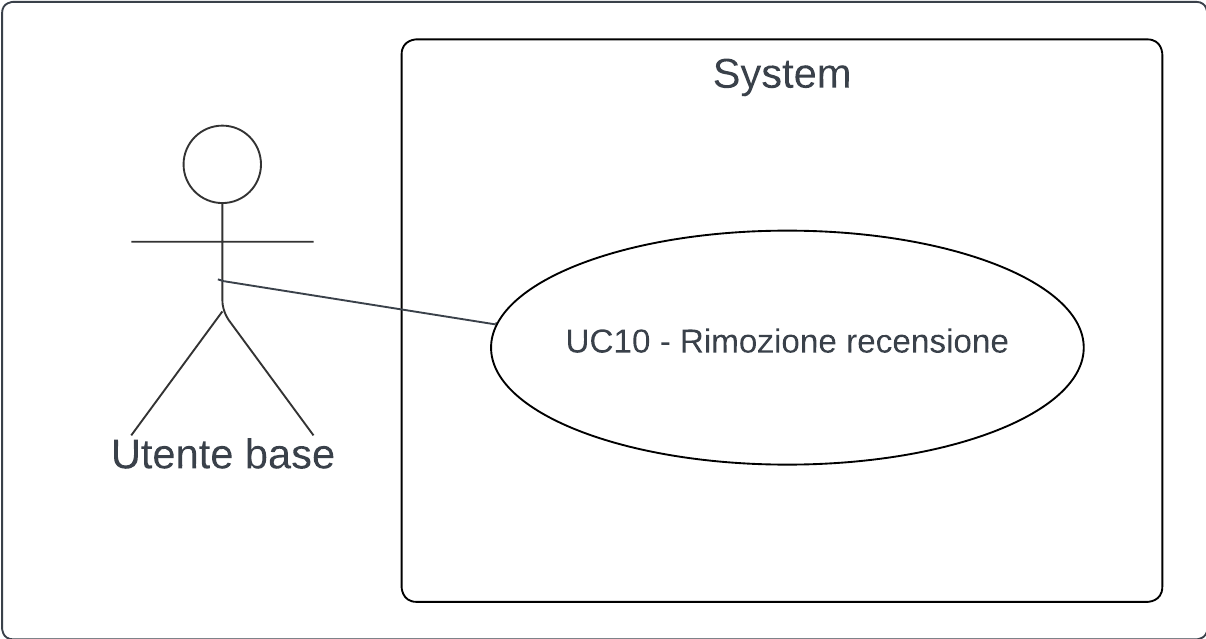
\includegraphics[width=0.75\linewidth]{ucd/UCD10.png}
\end{figure}
\textbf{Attori}:
\begin{itemize}
    \item Utente base
\end{itemize}
\textbf{Precondizioni}:
\begin{itemize}
    \item L'utente ha rilasciato in precedenza almeno una recensione (\nameref{usecase:7})
\end{itemize}
\textbf{Postcondizioni}:
\begin{itemize}
    \item L'utente ha rimosso la recensione desiderata
\end{itemize}
\textbf{Scenario principale}:
\begin{enumerate}
    \item L'utente seleziona il ristorante che aveva recensito in precedenza
    \item L'utente seleziona la sua recensione pubblicata in precedenza
    \item L'utente rimuove la recensione selezionata
\end{enumerate}
\newpage

%caso d'uso UC11 - Visualizzazione del menu' del ristorante
\subsection{UC11 - Visualizzazione del menu' ristorante} \label{usecase:11}
\begin{figure}[H]
    \centering
    \includegraphics[width=0.9\linewidth]{ucd/ucd11.png}
\caption{Visualizzazione del menu' ristorante}
\end{figure}
\textbf{Attori}:
\begin{itemize}
    \item Utente base.
\end{itemize}
\textbf{Precondizioni}:
\begin{itemize}
    \item L'utente ha scelto il menu' di un ristorante da visualizzare.
\end{itemize}
\textbf{Postcondizioni}:
\begin{itemize}
    \item L'utente ha visualizzato il menu' del ristorante.
\end{itemize}
\textbf{Scenario principale}:
\begin{enumerate}
    \item L'utente visualizza la lista dei piatti presenti nel menu';
    \item L’utente visualizza il piatto con relativo nome, prezzo e lista di ingredienti (\nameref{usecase:11_1}).
\end{enumerate}
\begin{comment}
% Forse non ci va perche non è un errore se la lista è vuota(?)
\textbf{Scenari alternativi}: % o secondari
\begin{enumerate}
    \item Il menu' è vuoto (non sono presenti piatti inseriti dall'amministratore oppure i criteri di ricerca non restituiscono piatti corrispondenti) e viene visualizzato un messaggio di errore
\end{enumerate}
\end{comment}

%caso d'uso UC11.1 - Visualizzazione piatto all'interno del menu'
\subsubsection{UC11.1 - Visualizzazione del piatto all'interno del menu'} \label{usecase:11_1}
\textbf{Attori}:
\begin{itemize}
    \item Utente generico.
\end{itemize}
\textbf{Precondizioni}:
\begin{itemize}
    \item L'utente ha scelto il menu' di un ristorante da visualizzare.
\end{itemize}
\textbf{Postcondizioni}:
\begin{itemize}
    \item L'utente ha visualizzato il singolo piatto all'interno del menu' del ristorante.
\end{itemize}
\textbf{Scenario principale}:
\begin{enumerate}
    \item L'utente visualizza il piatto con relativo nome, prezzo e lista di ingredienti.
\end{enumerate}
\newpage

%caso d'uso C12 - Login
\subsection{UC12 - Login} \label{usecase:12}
\begin{figure}[H]
    \centering
    \includegraphics[width=0.9\linewidth]{ucd/ucd12.png}
\end{figure}
\textbf{Attori}:
\begin{itemize}
    \item Utente non autenticato
\end{itemize}
\textbf{Precondizioni}:
\begin{itemize}
    \item L'utente ha già creato in precedenza un account base o amministratore
\end{itemize}
\textbf{Postcondizioni}:
\begin{itemize}
    \item L'utente viene riconosciuto dal $\textit{sistema}_G$ e quindi viene autenticato
\end{itemize}
\textbf{Scenario principale}:
\begin{enumerate}
    \item L'utente inserisce la propria email (\nameref{usecase:12_1})
    \item L'utente inserisce la password (\nameref{usecase:12_2})
    \item L'utente accede al $\textit{sistema}_G$ se l'email e password corrispondono
\end{enumerate}
\textbf{Scenari alternativi}:
\begin{enumerate}
    \item Se l'utente inserisce:
    \begin{enumerate}
        \item Email non valida
        \begin{enumerate}
            \item Manca il carattere "@"
            \item Campo vuoto
        \end{enumerate}
        \item Campo password vuoto
        \item Email o password non corretti
    \end{enumerate}
    \item Visualizza un errore
    \item Il $\textit{sistema}_G$ chiede se vuole recuperare la password
\end{enumerate}
\subsubsection{UC12.1 - Inserimento email} \label{usecase:12_1}
\textbf{Attori}:
\begin{itemize}
    \item Utente non autenticato
\end{itemize}
\textbf{Precondizioni}:
\begin{itemize}
    \item L'utente ha già creato in precedenza un account base o amministratore
\end{itemize}
\textbf{Postcondizioni}:
\begin{itemize}
    \item L'utente inserisce la propria email
\end{itemize}
\textbf{Scenario principale}:
\begin{enumerate}
    \item L'utente inserisce l'email
\end{enumerate}
\textbf{Scenari alternativi}:
\begin{enumerate}
    \item Se l'email non rispetta i seguenti criteri, visualizza un errore:
    \begin{enumerate}
        \item L'email deve avere il carattere "@"
        \item L'email deve contenere caratteri supportati
        \item L'email non deve essere vuota
    \end{enumerate}
\end{enumerate}
\subsubsection{UC12.2 - Inserimento password} \label{usecase:12_2}
\textbf{Attori}:
\begin{itemize}
    \item Utente non autenticato
\end{itemize}
\textbf{Precondizioni}:
\begin{itemize}
    \item L'utente ha già creato in precedenza un account base o amministratore
\end{itemize}
\textbf{Postcondizioni}:
\begin{itemize}
    \item L'utente inserisce la propria email
\end{itemize}
\textbf{Scenario principale}:
\begin{enumerate}
    \item L'utente inserisce la password
\end{enumerate}
\textbf{Scenari alternativi}:
\begin{enumerate}
    \item Se la password non rispetta i seguenti criteri, visualizza un errore:
    \begin{enumerate}
        \item La password deve contenere caratteri supportati
        \item La password non deve essere vuota
    \end{enumerate}
\end{enumerate}
\newpage

%caso d'uso C13 - Rimozione della $\textit{prenotazione}_G$ del tavolo
\subsection{UC13 - Annullamento prenotazione del tavolo} \label{usecase:13}
\begin{figure}[H]
\centering
\includegraphics[width=0.75\linewidth]{ucd/ucd13.png}
\caption{Annullamento prenotazione del tavolo}
\end{figure}
\textbf{Attori}:
\begin{itemize}
    \item Utente base.
\end{itemize}
\textbf{Precondizioni}:
\begin{itemize}
    \item L'utente deve aver effettuato una prenotazione di un tavolo (\nameref{usecase:23});
    \item L'utente ha selezionato la prenotazione che desidera disdire;
    \item La cancellazione può essere effettuata con al massimo un giorno di anticipo rispetto alla data della prenotazione.
\end{itemize}
\textbf{Postcondizioni}:
\begin{itemize}
    \item L'utente ha rimosso la sua prenotazione.
\end{itemize}
\textbf{Scenario principale}:
\begin{enumerate}
    \item L'utente conferma la cancellazione della prenotazione.
\end{enumerate}
\newpage

%caso d'uso 14 - Modifica informazioni account dell'amministratore (esempio coperti disponibili)
\subsection{UC14 - Modifica informazioni ristorante} \label{usecase:14}
\begin{figure}[H]
    \centering
    \includegraphics[width=0.9\linewidth]{ucd/ucd14.png}
\end{figure}
\textbf{Attori}:
\begin{itemize}
    \item \textit{Amministratore}_G
\end{itemize}
\textbf{Precondizioni}:
\begin{itemize}
    \item L'amministratore in precedenza deve avere inserito le informazioni di un ristorante (\nameref{usecase:2_1})
\end{itemize}
\textbf{Postcondizioni}:
\begin{itemize}
    \item L'amministratore ha modificato le informazioni del ristorante
\end{itemize}
\textbf{\textit{Scenario}_G principale}:
\begin{enumerate}
    \item Il sistema mostra le informazioni del ristorante dell'amministratore:
    \begin{enumerate}
        \item Nome ristorante
        \item Città
        \item Recapiti del ristorante
        \item Orario del ristorante
        \item Coperti disponibili
        \item Tipologia di cucina
    \end{enumerate}
    \item L'utente può modificare le informazioni del suo ristorante
    \item Il sistema registra le modifiche apportate alle informazioni del ristorante
\end{enumerate}
\newpage

%caso d'uso 15 - Visualizzazione piatti per l'amministratore
\subsection{UC15 - Visualizzazione lista prenotazioni (amministratore)} \label{usecase:15}
\begin{figure}[H]
    \centering
    \includegraphics[width=0.9\linewidth]{ucd/ucd15.png}
\end{figure}
\textbf{Attori}:
\begin{itemize}
    \item Amministratore
\end{itemize}
\textbf{Precondizioni}:
\begin{itemize}
    \item L'amministratore deve avere almeno un ristorante
\end{itemize}
\textbf{Postcondizioni}:
\begin{itemize}
    \item L'amministratore ha visualizzato la lista di prenotazioni in un giorno selezionato
\end{itemize}
\textbf{Scenario principale}:
\begin{enumerate}
   \item L'amministratore visualizza in un giorno selezionato (di default è la data corrente):
   \begin{enumerate}
       \item Gli ingredienti necessari per soddisfare la richiesta giornaliera di ordinazioni (\nameref{usecase:15_1})
       \item La lista delle prenotazioni in qualsiasi stato
       (\nameref{usecase:15_2})
   \end{enumerate}
\end{enumerate}
\begin{comment}
    \textbf{Scenari alternativi}: 
\begin{enumerate}
    \item La lista delle prenotazioni è vuota per il giorno selezionato, viene visualizzato il messaggio: "Prenotazioni non disponibili per il giorno selezionato"
\end{enumerate}
\end{comment}

%caso d'uso 15.1 - Visualizzazione lista ingredienti
\subsubsection{UC15.1 - Visualizzazione lista ingredienti giornalieri}\label{usecase:15_1}
\textbf{Attori}:
\begin{itemize}
    \item Amministratore
\end{itemize}
\textbf{Precondizioni}:
\begin{itemize}
    \item L'amministratore deve avere almeno un ristorante
\end{itemize}
\textbf{Postcondizioni}:
\begin{itemize}
    \item L'amministratore visualizza la lista degli ingredienti necessari per quella giornata
\end{itemize}
\textbf{Scenario principale}:
\begin{enumerate}
    \item L'utente visualizza la lista degli ingredienti necessari per quella giornata, viene riportato:
    \begin{enumerate}
        \item Nome dell'ingrediente
        \item Quantità dell'ingrediente
        \item Piatto associato all'ingrediente
    \end{enumerate}
\end{enumerate}

%caso d'uso 15.2 - Visualizzazione dettagli prenotazione
\subsubsection{UC15.2 - Visualizzazione dettagli prenotazione}\label{usecase:15_2}
\textbf{Attori}:
\begin{itemize}
    \item Amministratore.
\end{itemize}
\textbf{Precondizioni}:
\begin{itemize}
    \item L'amministratore è connesso al $\textit{sistema}_G$.
\end{itemize}
\textbf{Postcondizioni}:
\begin{itemize}
    \item L'amministratore visualizza i dettagli della $\textit{prenotazione}_G$ nella lista per il giorno selezionato.
\end{itemize}
\textbf{Scenario principale}:
\begin{enumerate}
    \item L'utente visualizza i dettagli della singola $\textit{prenotazione}_G$ presente nella lista ovvero:
    \begin{enumerate}
        \item Numero di persone associate;
        \item Stato della $\textit{prenotazione}_G$:
         \begin{enumerate}
           \item In corso (se `e ancora attiva) o terminata o annullata
            \item Accettata o rifiutata dall’amministratore o in attesa
       \end{enumerate}
    \item Giorno della $\textit{prenotazione}_G$;
    \item Orario della $\textit{prenotazione}_G$.
    \end{enumerate}
\end{enumerate}
\newpage

%caso d'uso 16 - Recupero password
\subsection{UC16 - Recupero password} \label{usecase:16}
\begin{figure}[H]
    \centering
    \includegraphics[width=0.8\linewidth]{ucd/ucd16.png}
    \caption{Recupero password}
\end{figure}
\textbf{Attori}:
\begin{itemize}
   \item Utente generico.
\end{itemize}
\textbf{Precondizioni}:
\begin{itemize}
    \item L'utente si è registrato in precedenza.(\nameref{usecase:1} \nameref{usecase:2})
\end{itemize}
\textbf{Postcondizioni}:
\begin{itemize}
    \item L'utente ha recuperato la propria password.
\end{itemize}
\textbf{Scenario principale}:
\begin{enumerate}
    \item Se l'utente non è autenticato inserisce l'email con cui si era registrato in precedenza;
    \item L'utente riceve una email dal $\textit{sistema}_G$ per il recupero password;
    \item L'utente, tramite un link nell'email accede ad una sezione che permette il cambio password.
\end{enumerate}
\newpage

%caso d'uso 17 - Visualizzare lista prenotazioni (utente base)
\subsection{UC17 - Visualizzazione lista prenotazioni (utente base)} \label{usecase:17}
\begin{figure}[H]
  \centering
  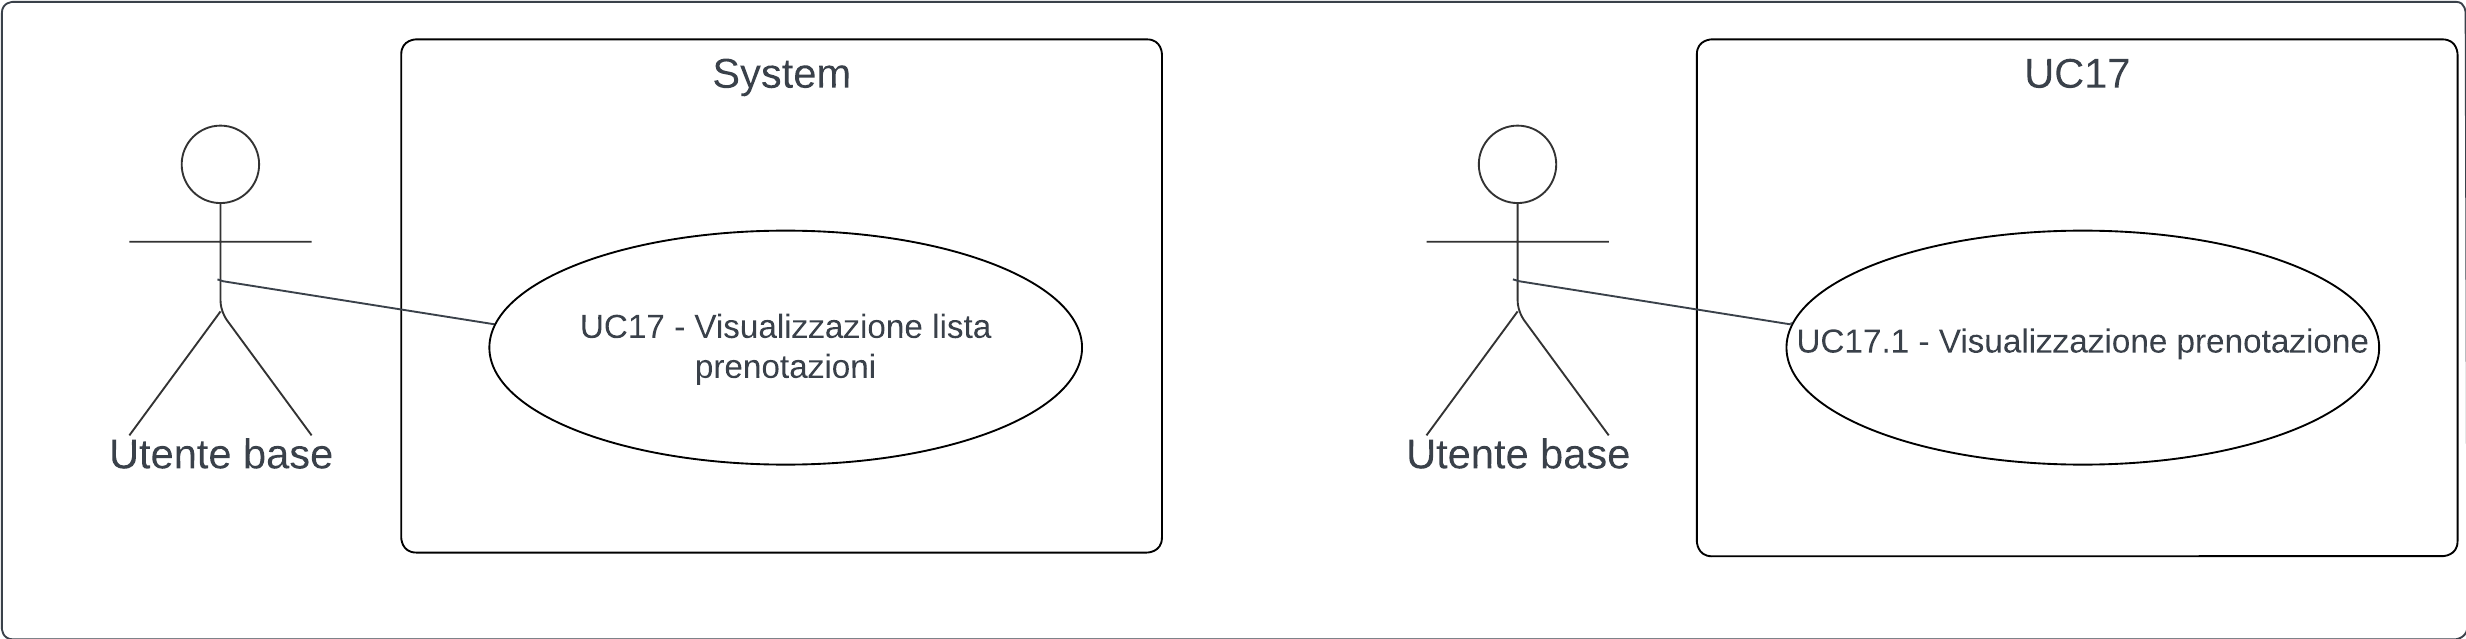
\includegraphics[width=1\textwidth]{ucd/UCD17.png}
  \caption{Visualizzazione lista prenotazioni (utente base)}
\end{figure}
\textbf{Attori}:
\begin{itemize}
    \item Utente base.
\end{itemize}
\textbf{Precondizioni}:
\begin{itemize}
    \item L'utente è connesso al sistema.
\end{itemize}
\textbf{Postcondizioni}:
\begin{itemize}
    \item L'utente visualizza una lista delle prenotazioni con le relative informazioni.
\end{itemize}
\textbf{Scenario principale}:
\begin{enumerate}
    \item L'utente visualizza una lista composta dalle prenotazioni effettuate in precedenza se presenti;
    \item Ogni voce della lista visualizza le informazioni relative alla specifica prenotazione (\nameref{usecase:17_1}).
\end{enumerate}
\begin{comment}
\textbf{Scenari alternativi}: 
\begin{enumerate}
    \item La lista delle prenotazioni è vuota, viene visualizzato il messaggio: "Non ci sono prenotazioni effettuate"
\end{enumerate}
\end{comment}

%caso d'uso 17.1 - Visualizzazione prenotazione
\subsubsection{UC17.1 - Visualizzazione prenotazione}\label{usecase:17_1}
\textbf{Attori}:
\begin{itemize}
    \item Utente base.
\end{itemize}
\textbf{Precondizioni}:
\begin{itemize}
    \item L'utente è connesso al sistema.
\end{itemize}
\textbf{Postcondizioni}:
\begin{itemize}
    \item L'utente ha visualizzato la singola prenotazione dalla lista.
\end{itemize}
\textbf{Scenario principale}:
\begin{enumerate}
    \item L'utente visualizza della singola prenotazione nella lista:
    \begin{enumerate}
        \item Il nome del ristorante dove è stata effettuata;
        \item La data della prenotazione;
        \item L'ora della prenotazione;
        \item Lo stato della prenotazione:
            \begin{itemize}
                \item In corso (se è ancora attiva) o terminata  o annullata;
                \item Accettata o rifiutata dall'amministratore o in attesa;
            \end{itemize}
        \item Quante persone sono state invitate.
    \end{enumerate}
\end{enumerate}
\newpage

%caso d'uso 18 - Applicazione coupon al conto finale
\subsection{UC18 - Applicazione coupon al conto} \label{usecase:18}
\begin{figure}[H]
    \centering
    \includegraphics[width=0.9\linewidth]{ucd/ucd18.png}
    \caption{Applicazione coupon al conto}
\end{figure}
\textbf{Attori}:
\begin{itemize}
    \item Utente base.
\end{itemize}
\textbf{Precondizioni}:
\begin{itemize}
    \item L'utente deve avere una $\textit{prenotazione}_G$ in corso;
    \item L'utente deve avere a disposizione un coupon da applicare al conto del ristorante.
\end{itemize}
\textbf{Postcondizioni}:
\begin{itemize}
    \item L'utente autenticato ha applicato il coupon.
\end{itemize}
\textbf{Scenario principale}:
\begin{enumerate}
    \item L'utente sceglie dalla lista delle prenotazioni una che sia in corso;
    \item L'utente inserisce il codice del coupon;
    \item Viene visualizzato il conto aggiornato.
\end{enumerate}
\textbf{Scenari alternativi}:
\begin{enumerate}
    \item Il coupon non è valido, viene visualizzato un messaggio di errore.
\end{enumerate}
\newpage

%caso d'uso 19 - Conferma $\textit{prenotazione}_G$ (utente amministratore)
\subsection{UC19 - Accettazione richiesta prenotazione}\label{usecase:19}
\begin{figure}[H]
    \centering
    \includegraphics[width=0.9\linewidth]{ucd/ucd19.png}
    \caption{Accettazione richiesta prenotazione}
\end{figure}
\textbf{Attori principali}:
\begin{itemize}
    \item Amministratore.
\end{itemize}
\textbf{Precondizioni}:
\begin{itemize}
    \item \`E arrivata almeno una richiesta di prenotazione da parte di un'utente base (\nameref{usecase:23}).
\end{itemize}
\textbf{Postcondizioni}:
\begin{itemize}
    \item L'amministratore ha accettato la richiesta;
    \item Il sistema ha aggiunto la prenotazione nell'area dedicata dell'utente che ha prenotato;
    \item Il sistema ha notificato gli utenti dell'accettazione della prenotazione.
\end{itemize}
\textbf{Scenario principale}:
\begin{enumerate}
    \item L'amministratore seleziona una richiesta di prenotazione;
    \item L'amministratore in base alla disponibilità del ristorante fornita dal sistema, accetta la prenotazione.
\end{enumerate}

\newpage

\begin{comment}
\subsection{UC19 - Conferma prenotazione (utente amministratore)}\label{usecase:10}
\textbf{Attori}:
\begin{itemize}
    \item Utente amministratore
\end{itemize}
\textbf{Precondizioni}:
\begin{itemize}
    \item L'utente amministratore si è autenticato all'interno del sistema.
    \item Vi deve essere almeno una prenotazione presente all'interno della lista associata al ristorante.
\end{itemize}
\textbf{Postcondizioni}:
\begin{itemize}
    \item L'amministratore ha confermato una prenotazione
\end{itemize}
\textbf{Scenario principale}:
\begin{enumerate}
    \item L'utente amministratore trova la lista delle prenotazioni (fare UC apposito?)
    \item L'utente amministratore sceglie una delle possibili prenotazioni da confermare e ne visualizza i dettagli associati (UC apposito per la visualizzazione di una prenotazione?)
    \item L'utente amministratore conferma la prenotazione.
\end{enumerate}
\textbf{Scenari secondari}:
\begin{itemize}
    \item nel caso in cui l'utente amministratore decida di non confermare la prenotazione, ritorna alla lista delle prenotazioni, lasciando la prenotazione inalterata.
\end{itemize}
\newpage
\end{comment}

%caso d'uso 20 - Rifiuto $\textit{prenotazione}_G$ (utente amministratore)
\subsection{UC20 - Rifiuto richiesta prenotazione}\label{usecase:20}
\begin{figure}[H]
    \centering
    \includegraphics[width=0.9\linewidth]{ucd/ucd20.png}
    \caption{Rifiuto richiesta prenotazione}
\end{figure}
\textbf{Attori principali}:
\begin{itemize}
    \item Amministratore.
\end{itemize}
\textbf{Precondizioni}:
\begin{itemize}
     \item \`E arrivata almeno una richiesta di $\textit{prenotazione}_G$ da parte di un'utente base (\nameref{usecase:23}).
\end{itemize}
\textbf{Postcondizioni}:
\begin{itemize}
    \item L'amministratore ha rifiutato la richiesta;
    \item Il $\textit{sistema}_G$ ha notificato gli utenti del rifiuto della $\textit{prenotazione}_G$.
\end{itemize}
\textbf{Scenario principale}:
\begin{enumerate}
    \item L'amministratore seleziona una richiesta di $\textit{prenotazione}_G$;
    \item L'amministratore in base alla disponibilità del ristorante fornita dal $\textit{sistema}_G$, rifiuta la $\textit{prenotazione}_G$.
\end{enumerate}
\newpage

%caso d'uso 21 - Visualizzazione recensioni e feedback
\subsection{UC21 - Visualizzazione recensioni}\label{usecase:21}
\begin{figure}[H]
    \centering
    \includegraphics[width=0.9\linewidth]{ucd/ucd21.png}
\end{figure}
\textbf{Attori}:
\begin{itemize}
    \item Utente generico
\end{itemize}
\textbf{Precondizioni}:
\begin{itemize}
    \item L'utente ha scelto un ristorante di cui vuole visualizzare le recensioni
\end{itemize}
\textbf{Postcondizioni}:
\begin{itemize}
    \item L'utente ha visualizzato le recensioni di un ristorante
\end{itemize}
\textbf{Scenario principale}:
\begin{enumerate}
    \item L'utente può visualizzare le recensioni associate al ristorante scelto
    \item L'utente visualizza per ogni recensione:
    \begin{enumerate}
        \item Votazione in stelle
        \item La recensione
        \item Nome utente che l'ha rilasciata
        \item La data del rilascio
    \end{enumerate}
\end{enumerate}

\newpage

\subsubsection{UC21.1 - Visualizzazione informazioni recensione}\label{usecase:21_1}
\textbf{Attori}:
\begin{itemize}
    \item Utente generico
\end{itemize}
\textbf{Precondizioni}:
\begin{itemize}
    \item L'utente ha scelto un ristorante di cui vuole visualizzare le recensioni
\end{itemize}
\textbf{Postcondizioni}:
\begin{itemize}
    \item L'utente ha visualizzato le informazioni dettagliate di una recensione del ristorante selezionato.
\end{itemize}
\textbf{Scenario principale}:
\begin{enumerate}
    \item L'utente visualizza le informazioni dettagliate di una recensione associata al ristorante scelto.
    \item Per ogni recensione, l'utente visualizza:
    \begin{enumerate}
        \item La votazione in stelle assegnata alla recensione.
        \item Il testo della recensione.
        \item Il nome dell'utente che ha rilasciato la recensione.
        \item La data in cui la recensione è stata rilasciata.
    \end{enumerate}
\end{enumerate}

\newpage

%caso d'uso 22 - Risposta ad una recensione da parte dell'amministratore
\subsection{UC22 - Gestione feedback (\textit{Amministratore}_G)}\label{usecase2:22}
\begin{figure}[H]
    \centering
    \includegraphics[width=0.9\linewidth]{ucd/ucd22.png}
\end{figure}
\textbf{Attori}:
\begin{itemize}
    \item \textit{Amministratore}_G
\end{itemize}
\textbf{Precondizioni}:
\begin{itemize}
    \item Sono state rilasciate recensioni ad almeno un ristorante di cui l'amministratore detiene i privilegi di amministratore
\end{itemize}
\textbf{Postcondizioni}:
\begin{itemize}
    \item L'amministratore visualizza le recensioni e le eventuali risposte
\end{itemize}
\textbf{\textit{Scenario}_G principale}:
\begin{enumerate}
    \item L'amministratore visualizza la lista delle recensioni del ristorante di cui è amministratore (\nameref{usecase:22_1})
    \item L'amministratore seleziona la recensione a cui dovrà rispondere
    \item L'amministratore risponde alla recensione selezionata tramite un messaggio di testo (\nameref{usecase:22_2})
\end{enumerate}

\subsubsection{UC22.1 - Visualizza recensioni}\label{usecase:22_1}
\textbf{Attori}:
\begin{itemize}
    \item Amministratore
\end{itemize}
\textbf{Precondizioni}:
\begin{itemize}
    \item Sono state rilasciate recensioni ad almeno un ristorante di cui l'amministratore detiene i privilegi di amministratore
\end{itemize}
\textbf{Postcondizioni}:
\begin{itemize}
    \item L'amministratore visualizza le recensioni
\end{itemize}
\textbf{Trigger}:
L'amministratore vuole visualizzare le recensioni\\
\textbf{Scenario principale}:
\begin{enumerate}
    \item Viene visualizza la lista delle recensioni con le seguenti informazioni:
    \begin{enumerate}
        \item Username del profilo che l'ha rilasciata
        \item Giorno e ora
        \item Testo della recensione
    \end{enumerate}
\end{enumerate}
\subsubsection{UC22.2 - Risposta alla recensione}\label{usecase:22_2}
\textbf{Attori}:
\begin{itemize}
    \item Amministratore
\end{itemize}
\textbf{Precondizioni}:
\begin{itemize}
    \item L'amministratore ha selezionato una recensione a cui rispondere
\end{itemize}
\textbf{Postcondizioni}:
\begin{itemize}
    \item L'amministratore ha risposto alla recensione
\end{itemize}
\textbf{Trigger}:
L'amministratore vuole rispondere ad una recensione\\
\textbf{Scenario principale}:
\begin{enumerate}
    \item L'amministratore deve inserire un testo valido da inserire come risposta
\end{enumerate}
\textbf{Scenario alternativo}:
\begin{enumerate}
    \item Se il testo è: 
    \begin{enumerate}
        \item Vuoto
        \item Contiene caratteri non ammessi
        \item Supera una dimensione di 255 caratteri
    \end{enumerate}
    \item Allora la recensione non può essere pubblicata
    \item Si visualizza l'errore
\end{enumerate}

% $\textit{caso d'uso}_G$ 23
\subsection{UC23 - Prenotazione tavolo}\label{usecase:23}

\begin{figure}[H]
  \centering
  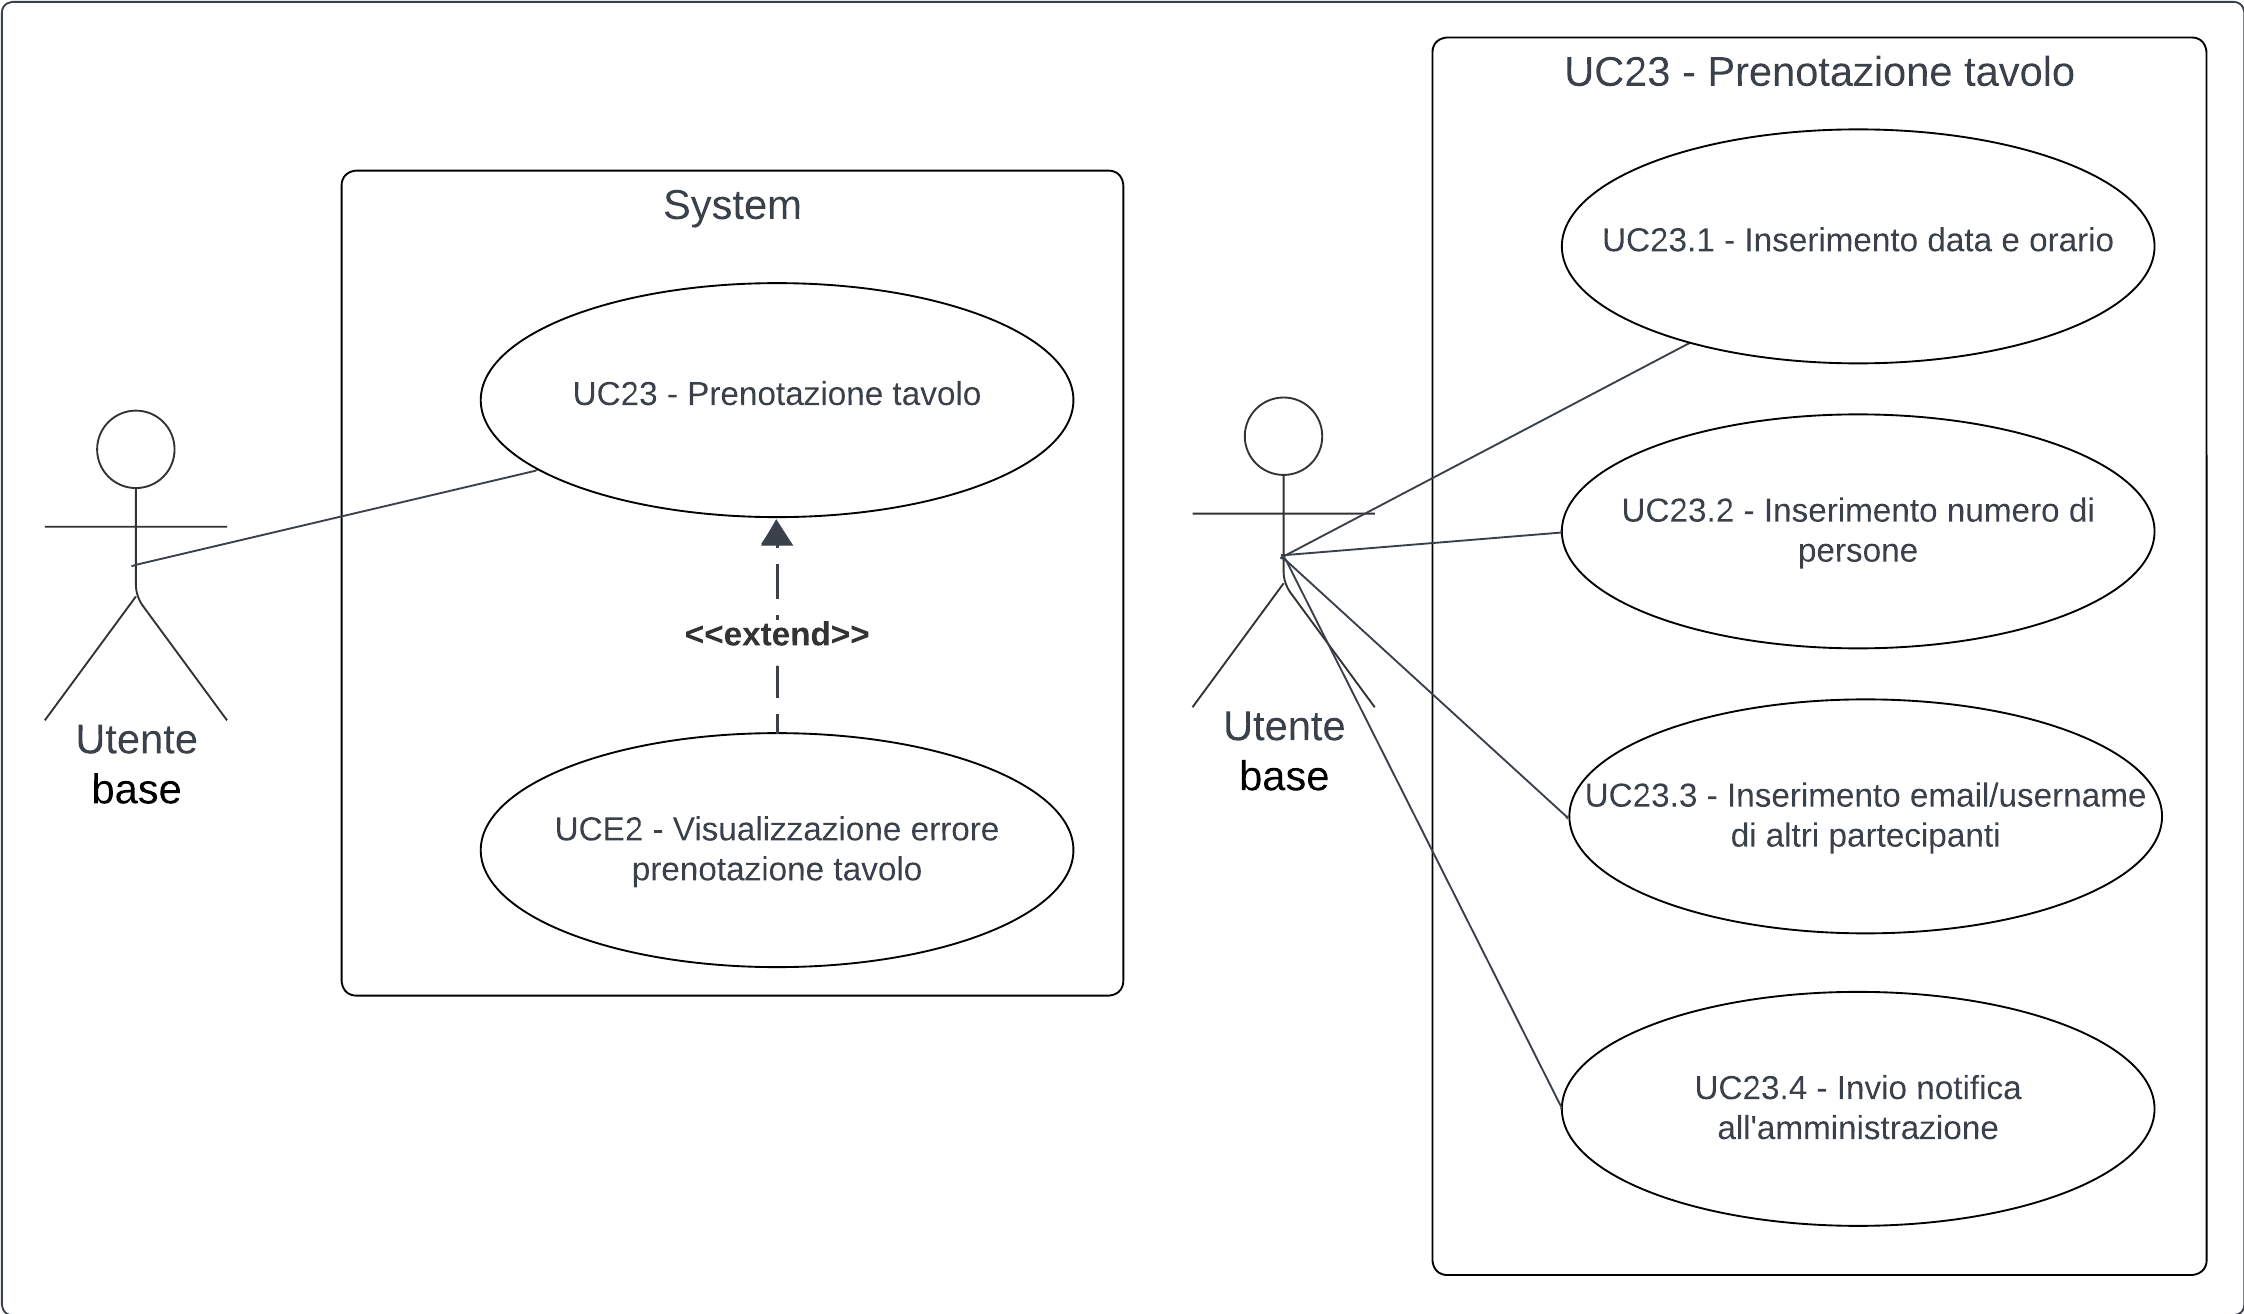
\includegraphics[width=0.9\linewidth]{ucd/UCD23.png}
\end{figure}

\textbf{Attori principali}:
\begin{itemize}
    \item Utente base autenticato
\end{itemize}
\textbf{Precondizione}:
\begin{itemize}
    \item L'utente è autenticato ed è riconosciuto come utente base
    \item L'utente ha già selezionato il ristorante tramite la ricerca ristorante \nameref{usecase:24}
\end{itemize}
\textbf{Postcondizione}:
\begin{itemize}
    \item L'utente ha richiesto una $\textit{Prenotazione}_G$ in un ristorante
    \item Il $\textit{Sistema}_G$ ha inviato una notifica al ristorante selezionato
\end{itemize}
\textbf{Trigger}:
\begin{itemize}
    \item L'utente vuole prenotare un tavolo nel ristorante selezionato
\end{itemize}
\textbf{Scenario principale}:
\begin{enumerate}
    \item L'utente inserisce nella query di ricerca la data.
    \item L'utente specifica l'orario di arrivo.
    \item L'utente specifica il numero di persone.
    \item L'utente specifica, inserendo username/email utente, chi sono le altre persone al tavolo.
    \item Il $\textit{Sistema}_G$ invia una notifica di una richiesta di $\textit{Prenotazione}_G$ agli amministratori del ristorante.
\end{enumerate}
\textbf{Scenari alternativi}:
\begin{itemize}
    \item Se si verifica:
    \begin{enumerate}
        \item L'utente decide di cancellare la prenotazione.
        \item Il ristorante non possiede tavoli liberi all'ora scelta.
        \item Il ristorante non possiede abbastanza posti per quell'ora.
    \end{enumerate}
    \item L'utente visualizza un messaggio di errore
    \item La $\textit{Prenotazione}_G$ viene cancellata
\end{itemize}



\subsubsection{UC23.1 - Inserimento data e ora}\label{usecase:23_1}
\textbf{Attori}:
\begin{itemize}
    \item Utente base autenticato
\end{itemize}
\textbf{Precondizioni}:
\begin{itemize}
    \item L'utente è autenticato ed è riconosciuto come utente base.
    \item L'utente ha già selezionato il ristorante tramite la ricerca ristorante \nameref{usecase:24}
\end{itemize}
\textbf{Postcondizioni}:
\begin{itemize}
    \item L'utente ha inserito correttamente la data e l'orario di arrivo per la prenotazione
\end{itemize}
\textbf{Scenario principale}:
\begin{enumerate}
    \item L'utente inserisce la data desiderata per la $\textit{Prenotazione}_G$ nel formato appropriato
    \item L'utente specifica l'orario di arrivo previsto nel formato appropriato.
\end{enumerate}



\subsubsection{UC23.2 - Inserimento numero di persone}\label{usecase:23_2}
\textbf{Attori}:
\begin{itemize}
    \item Utente base autenticato
\end{itemize}
\textbf{Precondizioni}:
\begin{itemize}
    \item L'utente è autenticato ed è riconosciuto come utente base.
    \item L'utente ha già selezionato il ristorante tramite la ricerca ristorante \nameref{usecase:24}
\end{itemize}
\textbf{Postcondizioni}:
\begin{itemize}
    \item L'utente ha inserito correttamente il numero di persone per la prenotazione.
\end{itemize}
\textbf{Scenario principale}:
\begin{enumerate}
    \item L'utente specifica il numero di persone che parteciperanno alla prenotazione.
\end{enumerate}


\subsubsection{UC23.3 - Inserimento email/username di altri partecipanti}\label{usecase:23_3}
\textbf{Attori}:
\begin{itemize}
    \item Utente base autenticato
\end{itemize}
\textbf{Precondizioni}:
\begin{itemize}
    \item L'utente è autenticato ed è riconosciuto come utente base.
    \item L'utente ha già selezionato il ristorante tramite la ricerca ristorante \nameref{usecase:24}
\end{itemize}
\textbf{Postcondizioni}:
\begin{itemize}
    \item L'utente ha inserito correttamente le informazioni degli altri partecipanti alla prenotazione.
\end{itemize}
\textbf{Scenario principale}:
\begin{enumerate}
    \item L'utente specifica, inserendo l'username/email degli altri partecipanti al tavolo, chi sono le altre persone coinvolte nella prenotazione.
\end{enumerate}


\subsubsection{UC23.4 - Invio notifica all'amministratore
}\label{usecase:23_4}
\textbf{Attori}:
\begin{itemize}
    \item Utente base autenticato
\end{itemize}
\textbf{Precondizioni}:
\begin{itemize}
    \item L'utente è autenticato ed è riconosciuto come utente base.
    \item L'utente ha già selezionato il ristorante tramite la ricerca ristorante \nameref{usecase:24}
    \item L'utente ha inserito correttamente tutte le informazioni necessarie per la prenotazione.
\end{itemize}
\textbf{Postcondizioni}:
\begin{itemize}
    \item Il $\textit{Sistema}_G$ ha inviato una notifica di una richiesta di $\textit{Prenotazione}_G$ agli amministratori del ristorante selezionato.
\end{itemize}
\textbf{Scenario principale}:
\begin{enumerate}
    \item Dopo aver completato l'inserimento di tutte le informazioni richieste, il $\textit{Sistema}_G$ invia una notifica di una richiesta di $\textit{Prenotazione}_G$ agli amministratori del ristorante selezionato.
\end{enumerate}



\newpage

\subsection{UC24 - Ricerca ristorante}\label{usecase:24}

\begin{figure}[H]
    \centering
    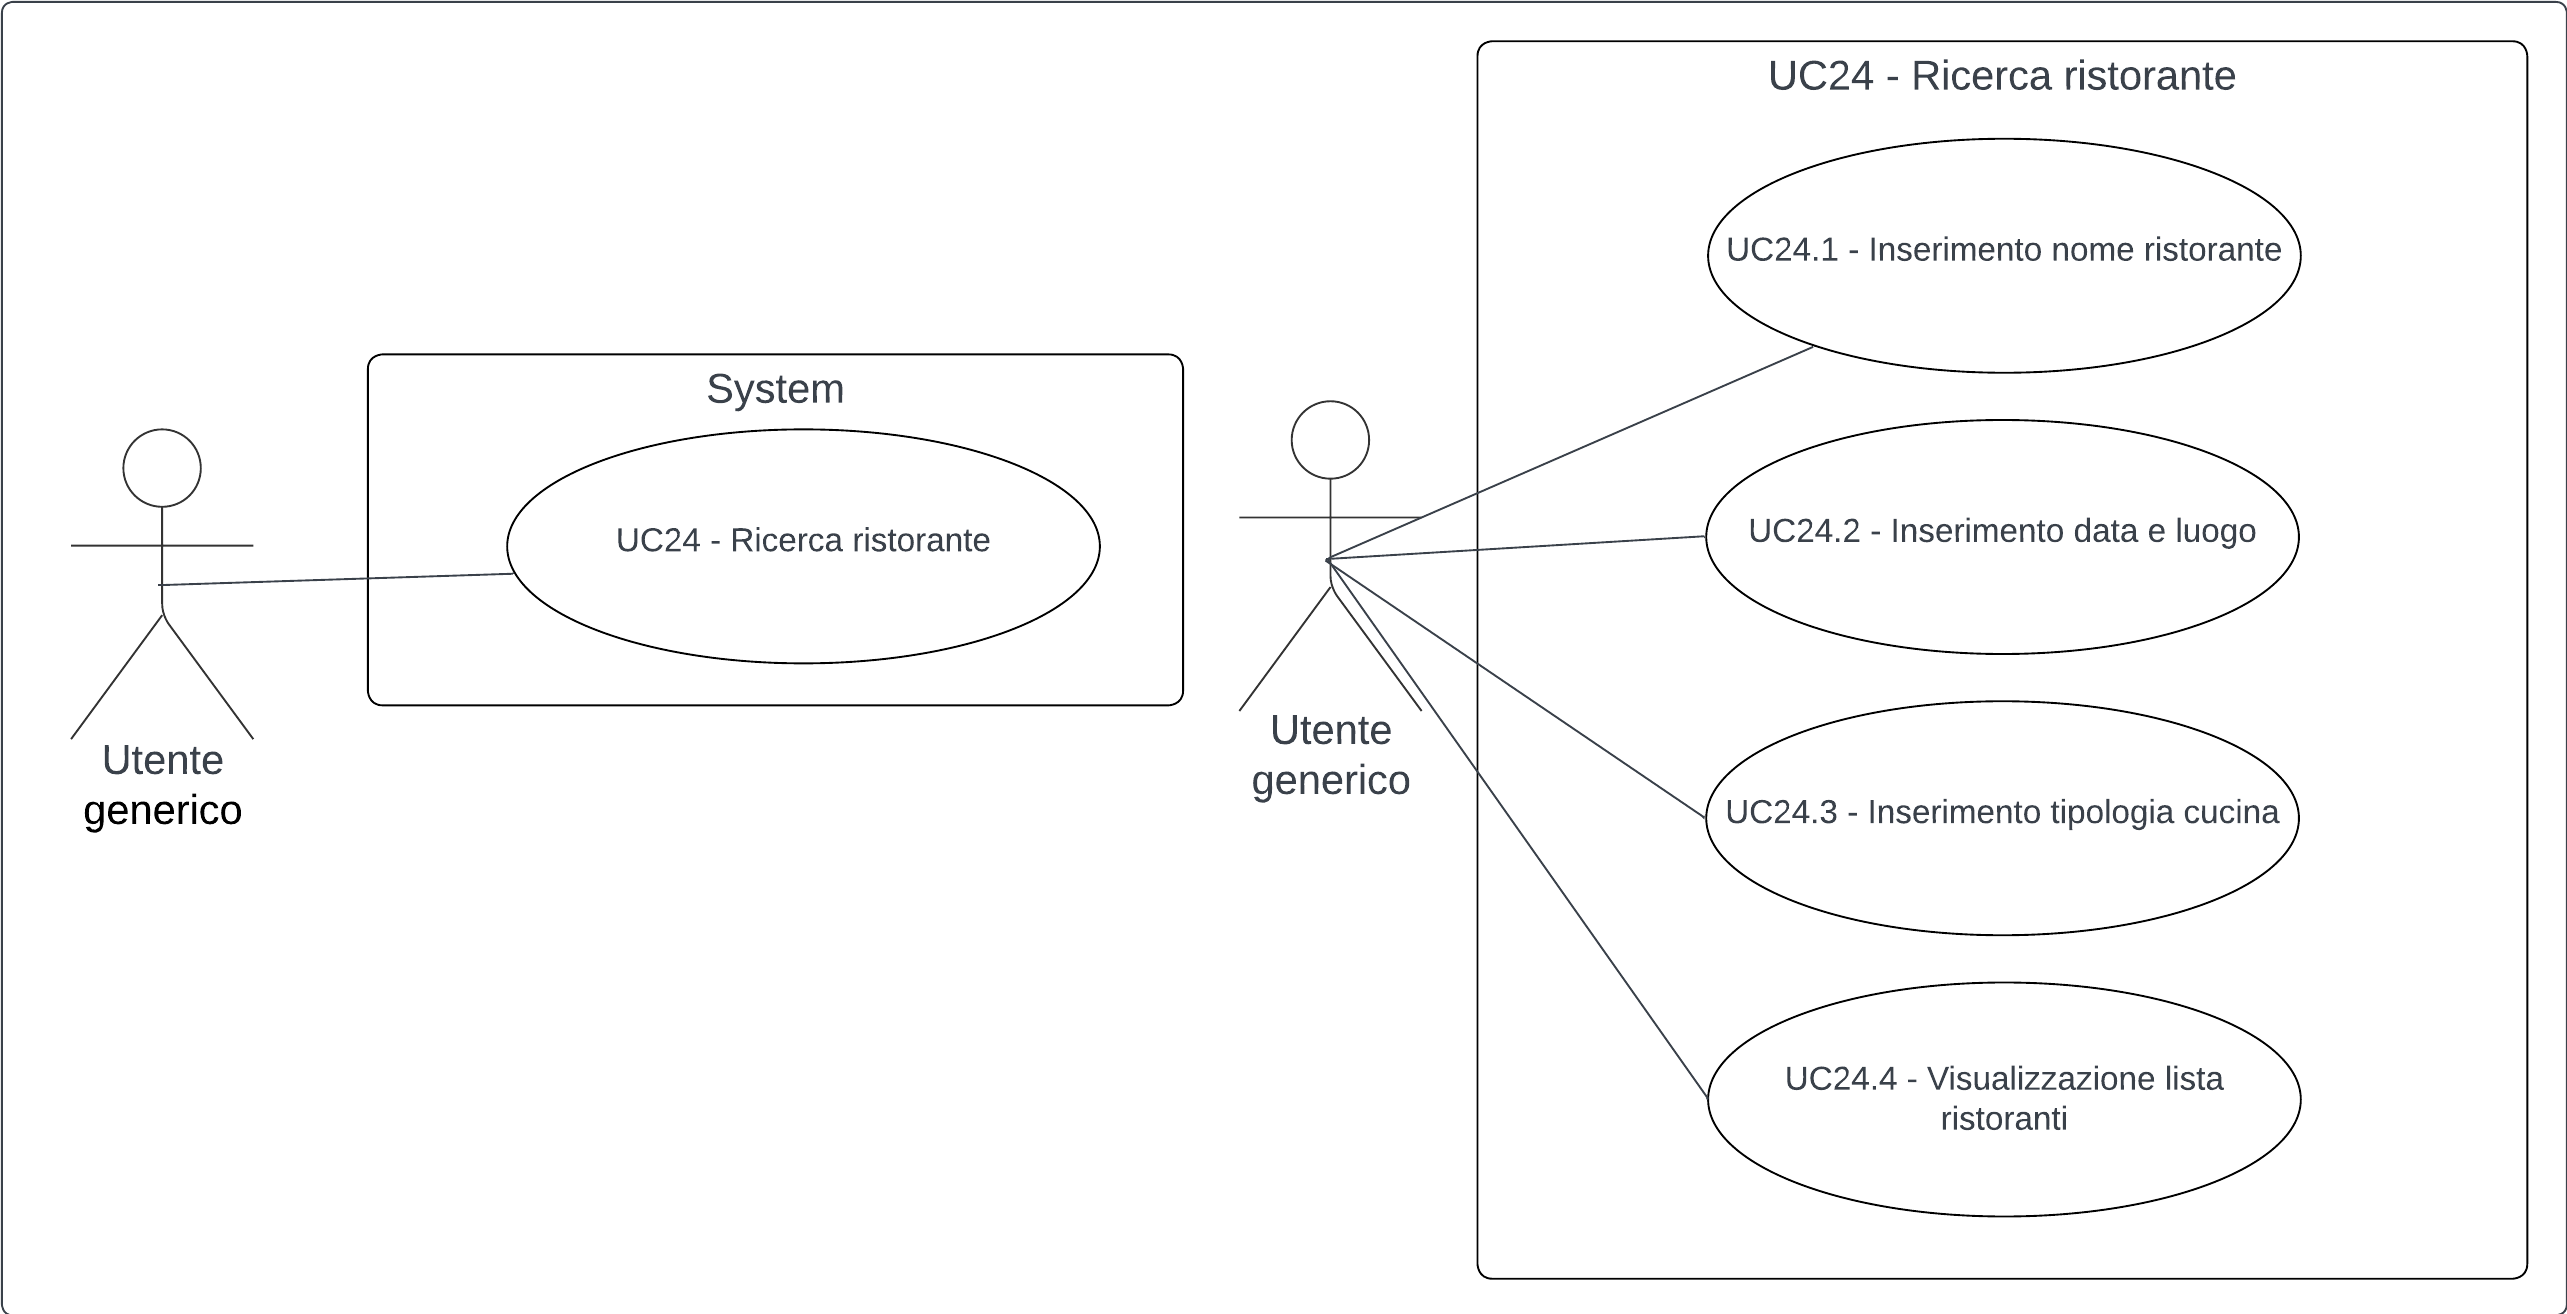
\includegraphics[width=0.9\linewidth]{ucd/UCD24.png}
    \caption{Ricerca ristorante}
\end{figure}

\textbf{Attori}:
\begin{itemize}
    \item Utente generico.
\end{itemize}
\textbf{Precondizioni}:
\begin{itemize}
    \item L'utente generico è connesso al $\textit{sistema}_G$.
\end{itemize}
\textbf{Postcondizioni}:
\begin{itemize}
    \item L'utente visualizza una lista di ristoranti che corrispondono ai criteri di ricerca.
\end{itemize}
\textbf{Scenario principale}:
\begin{enumerate}
    \item L'utente può ricercare il ristorante inserendo:
    \begin{itemize}
        \item Il nome (\nameref{usecase:24_1});
        \item La data e il luogo per escludere ristoranti chiusi(\nameref{usecase:24_2})
        \item Il tipo di cucina(\nameref{usecase:24_3});
    \end{itemize}
    \item L'utente conferma;
    \item L'utente visualizza la lista dei ristoranti che rispettano tali criteri (\nameref{usecase:24_4}).
\end{enumerate}

\subsubsection{UC24.1 - Inserimento nome ristorante
}\label{usecase:24_1}
\textbf{Attori}:
\begin{itemize}
    \item Utente generico.
\end{itemize}
\textbf{Precondizioni}:
\begin{itemize}
    \item L'utente generico è connesso al $\textit{sistema}_G$.
\end{itemize}
\textbf{Postcondizioni}:
\begin{itemize}
    \item L'utente ha inserito correttamente il nome del ristorante per la ricerca.
\end{itemize}
\textbf{Scenario principale}:
\begin{enumerate}
    \item L'utente inserisce il nome del ristorante che desidera cercare.
\end{enumerate}

\subsubsection{UC24.2 - Inserimento data e luogo
}\label{usecase:24_2}
\textbf{Attori}:
\begin{itemize}
    \item Utente generico.
\end{itemize}
\textbf{Precondizioni}:
\begin{itemize}
    \item L'utente generico è connesso al $\textit{sistema}_G$.
\end{itemize}
\textbf{Postcondizioni}:
\begin{itemize}
    \item L'utente ha inserito correttamente la data e/o il luogo per la ricerca dei ristoranti.
\end{itemize}
\textbf{Scenario principale}:
\begin{enumerate}
    \item L'utente inserisce la data per escludere i ristoranti chiusi;
    \item L'utente inserisce il luogo desiderato per la ricerca dei ristoranti.
\end{enumerate}


\subsubsection{UC24.3 - Inserimento tipologia cucina
}\label{usecase:24_3}
\textbf{Attori}:
\begin{itemize}
    \item Utente generico.
\end{itemize}
\textbf{Precondizioni}:
\begin{itemize}
    \item L'utente generico è connesso al $\textit{sistema}_G$.
\end{itemize}
\textbf{Postcondizioni}:
\begin{itemize}
    \item L'utente ha inserito correttamente la tipologia di cucina desiderata per la ricerca dei ristoranti.
\end{itemize}
\textbf{Scenario principale}:
\begin{enumerate}
    \item L'utente specifica il tipo di cucina che desidera cercare nei ristoranti.
\end{enumerate}


\subsubsection{UC24.4 - Visualizzazione lista ristoranti
}\label{usecase:24_4}
\textbf{Attori}:
\begin{itemize}
    \item Utente generico.
\end{itemize}
\textbf{Precondizioni}:
\begin{itemize}
    \item L'utente generico è connesso al $\textit{sistema}_G$;
    \item L'utente ha inserito correttamente tutti i criteri di ricerca per i ristoranti.
\end{itemize}
\textbf{Postcondizioni}:
\begin{itemize}
    \item L'utente visualizza una lista di ristoranti che corrispondono ai criteri di ricerca.
\end{itemize}
\textbf{Scenario principale}:
\begin{enumerate}
    \item Dopo aver confermato i criteri di ricerca, l'utente visualizza la lista dei ristoranti che rispettano tali criteri. Per ogni ristorante si visualizza:
    \begin{itemize}
        \item Il nome;
        \item La città e l'indirizzo.
    \end{itemize}
\end{enumerate}



\newpage

% $\textit{caso d'uso}_G$ 25 Inserimento intolleranze
\subsection{UC25 - Modifica allergie e intolleranze}\label{usecase:25}
\begin{figure}[H]
    \centering
    \includegraphics[width=0.75\linewidth]{ucd/ucd25.png}
    \caption{Modifica allergie e intolleranze}
\end{figure}
\textbf{Attori principali}:
\begin{itemize}
    \item Utente base.
\end{itemize}
\textbf{Precondizioni}:
\begin{itemize}
    \item L'utente è connesso al $\textit{sistema}_G$.
\end{itemize}
\textbf{Postcondizioni}:
\begin{itemize}
    \item L'utente ha modificato con successo la lista delle intolleranze e allergie.
\end{itemize}
\textbf{Scenario principale}:
\begin{enumerate}
    \item L'utente inserisce le proprie allergie se presenti (\nameref{usecase:25_1});
    \item L'utente inserisce le proprie intolleranze se presenti (\nameref{usecase:25_2}).
\end{enumerate}

  
\subsubsection{UC25.1 - Inserimento allergie}\label{usecase:25_1}
\textbf{Attori}:
\begin{itemize}
    \item Utente base.
\end{itemize}
\textbf{Precondizioni}:
\begin{itemize}
    \item L'utente sta modificando le informazioni del suo profilo.
\end{itemize}
\textbf{Postcondizioni}:
\begin{itemize}
    \item L'utente ha inserito con successo le proprie allergie nel suo profilo.
\end{itemize}
\textbf{Scenario principale}:
\begin{enumerate}
    \item L'utente inserisce le proprie allergie, se presenti, nel campo dedicato durante la modifica del suo profilo.
\end{enumerate}

\subsubsection{UC25.2 - Inserimento intolleranze}\label{usecase:25_2}
\textbf{Attori}:
\begin{itemize}
    \item Utente base.
\end{itemize}
\textbf{Precondizioni}:
\begin{itemize}
    \item L'utente sta modificando le informazioni del suo profilo.
\end{itemize}
\textbf{Postcondizioni}:
\begin{itemize}
    \item L'utente ha inserito con successo le proprie intolleranze nel suo profilo.
\end{itemize}
\textbf{Scenario principale}:
\begin{enumerate}
    \item L'utente inserisce le proprie intolleranze, se presenti, nel campo dedicato durante la modifica del suo profilo.
\end{enumerate}

 

\newpage

% $\textit{caso d'uso}_G$ 26 Inserimento informazioni utente
\subsection{UC26 - Modifica informazioni utente}\label{usecase:26}
\begin{figure}[H]
\centering
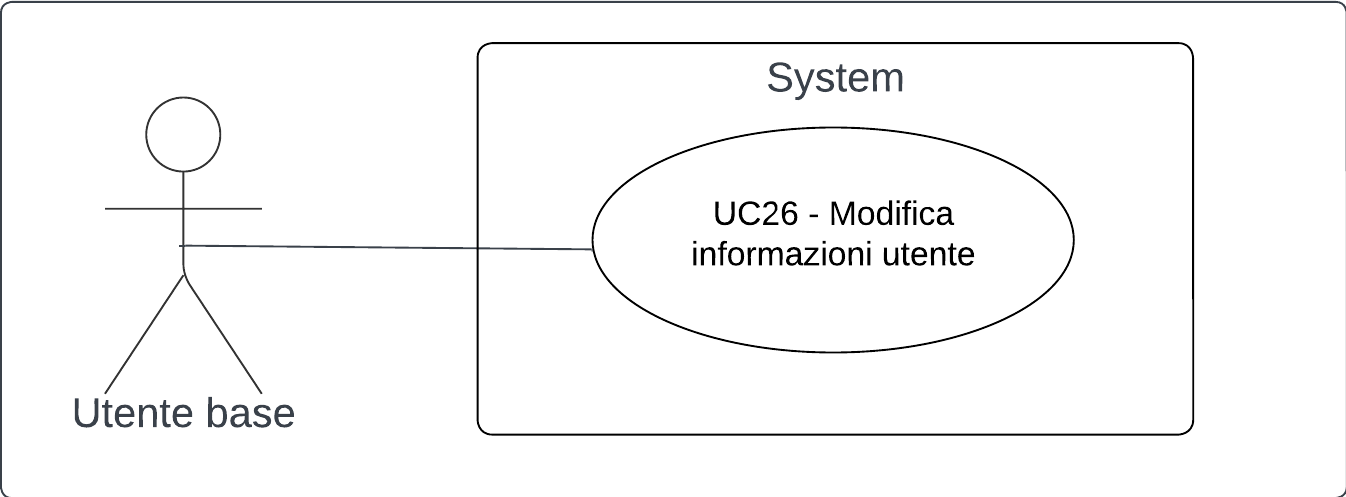
\includegraphics[width=0.75\linewidth]{ucd/UCD26}
\end{figure}
\textbf{Attori}:
\begin{itemize}
    \item Utente base
\end{itemize}
\textbf{Precondizioni}:
\begin{itemize}
    \item L'utente deve essere autenticato
\end{itemize}
\textbf{Postcondizioni}:
\begin{itemize}
    \item L'utente ha inserito le informazioni
\end{itemize}
\textbf{Scenario principale}:
\begin{enumerate}
    \item L'utente inserisce il suo nome
    \item L'utente inserisce il suo cognome
    \item L'utente inserisce un email valida
    \item l'utente inserisce la sua password
\end{enumerate}
\textbf{Scenari alternativi}:
\begin{enumerate}
    \item Nel caso in cui l'email sia già presente all'interno del sistema, l'utente viene notificato attraverso un messaggio visivo.
    \item Viene data la possibilità all'utente di scegliere un'email valida.
\end{enumerate}
\newpage

% $\textit{caso d'uso}_G$ 27 Logout
\subsection{UC27 - Logout}\label{usecase:27}
\begin{figure}[H]
\centering
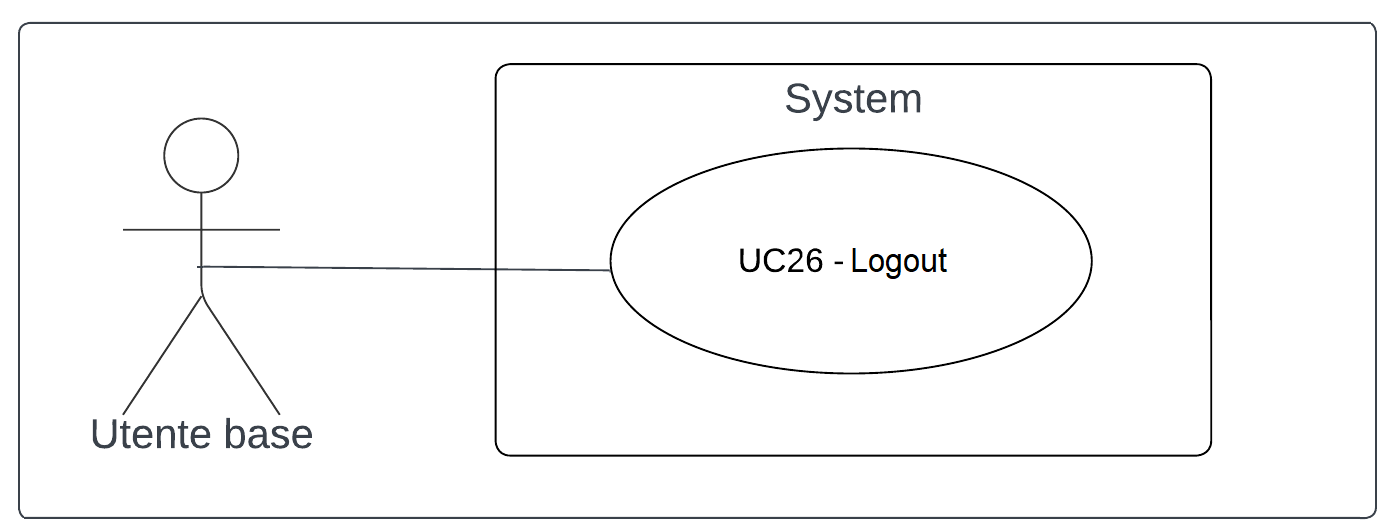
\includegraphics[width=0.75\linewidth]{ucd/UCD27.png}
\end{figure}
\textbf{Attori}:
\begin{itemize}
    \item Utente autenticato
\end{itemize}
\textbf{Precondizioni}:
\begin{itemize}
    \item L'utente è autenticato nel sistema
\end{itemize}
\textbf{Postcondizioni}:
\begin{itemize}
    \item L'utente è stato disconnesso dal $\textit{sistema}_G$ e non può accedere a funzionalità riservate agli utenti autenticati fino a quando non esegue nuovamente l'accesso.
\end{itemize}
\textbf{Scenario principale}:
\begin{enumerate}
    \item L'utente seleziona l'opzione di logout dal sistema.
    \item Il $\textit{sistema}_G$ conferma la richiesta di logout.
    \item Il $\textit{sistema}_G$ termina la sessione dell'utente e reindirizza l'utente alla pagina di accesso.
\end{enumerate}

\newpage

% $\textit{caso d'uso}_G$ 28 Annullamento ordinazione
\subsection{UC28 - Annullamento dell'ordinazione}\label{usecase:28}
\begin{figure}[H]
    \centering
    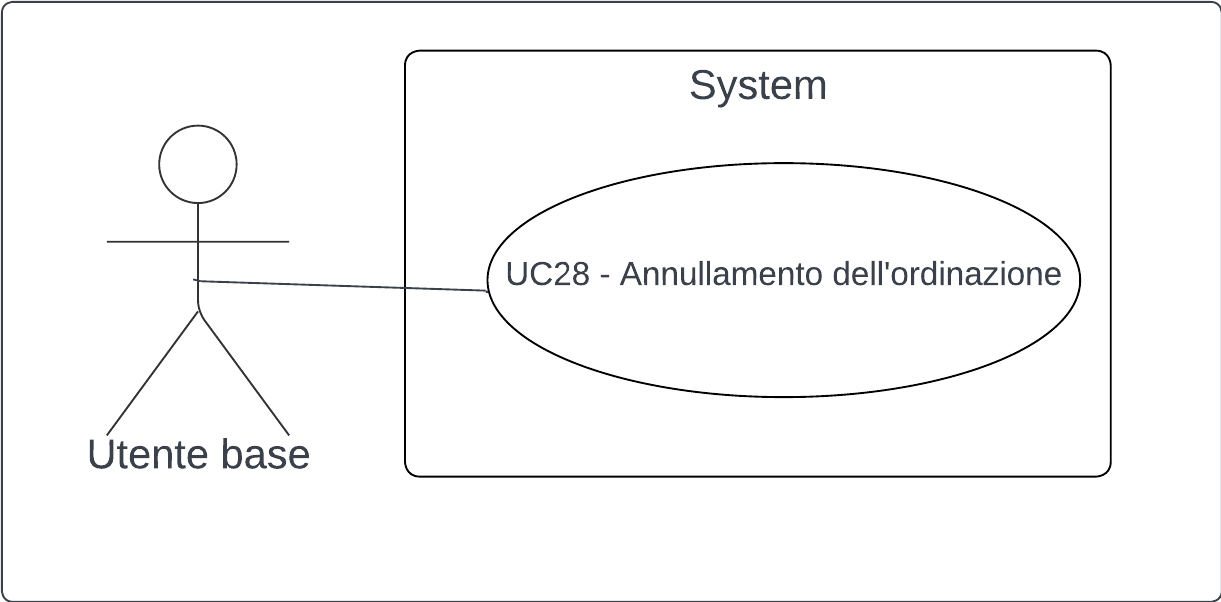
\includegraphics[width=0.9\linewidth]{ucd/UCD28.png}
\end{figure}
\textbf{Attori}:
\begin{itemize}
    \item Utente base
\end{itemize}
\textbf{Precondizioni}:
\begin{itemize}
    \item L'utente è autenticato
    \item L'utente ha creato un'ordinazione collaborativa (\nameref{usecase:3})
    \item Il tempo utile per annullare l'ordinazione non è scaduto
\end{itemize}
\textbf{Postcondizioni}:
\begin{itemize}
    \item L'utente ha annullato l'ordinazione collaborativa dei pasti e la $\textit{Prenotazione}_G$ si trova senza ordinazioni
\end{itemize}
\textbf{Scenario principale}:
\begin{enumerate}
    \item L'utente sceglie l'opzione di annullamento dell'ordinazione collaborativa
    \item Il $\textit{Sistema}_G$ annulla l'ordinazione associate alla $\textit{Prenotazione}_G$ e invia una notifica a tutti gli utenti associati a quella $\textit{Prenotazione}_G$
\end{enumerate}
\newpage

\begin{comment}
\subsection{UC29 - Ordinazione piatto}\label{usecase:29}

\begin{figure}[H]
    \centering
    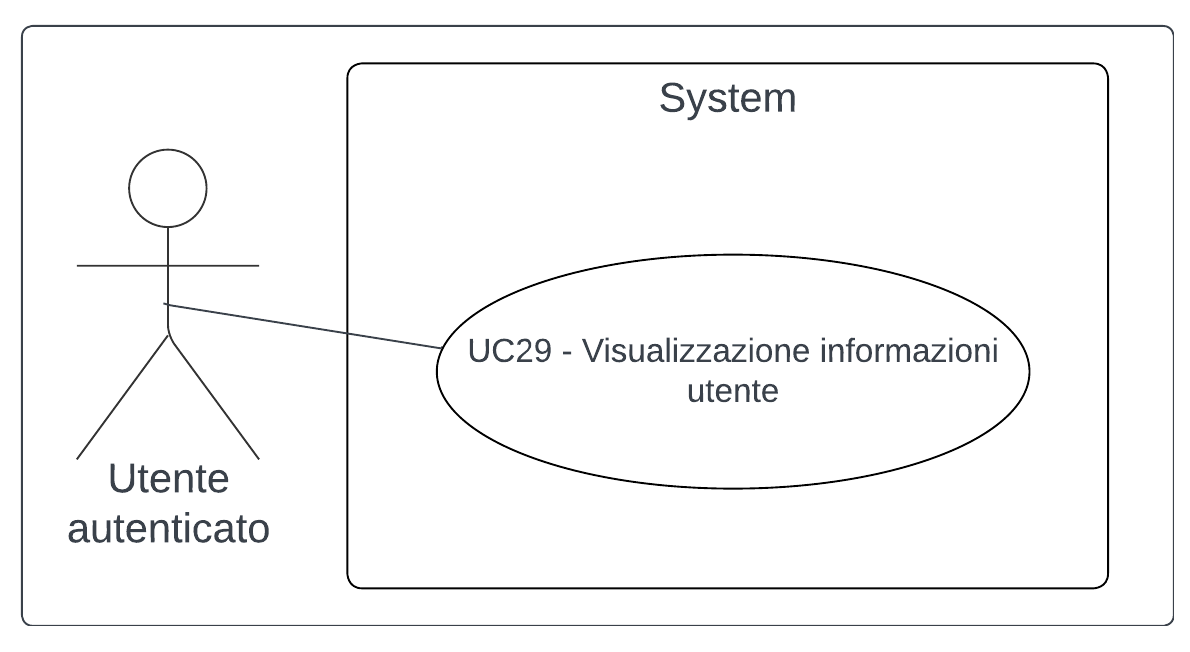
\includegraphics[width=0.9\linewidth]{ucd/UCD29.png}
\end{figure}

\textbf{Attori}:
\begin{itemize}
    \item Utente base autenticato
\end{itemize}
\textbf{Precondizioni}:
\begin{itemize}
    \item L'utente è autenticato dal $\textit{Sistema}_G$ 
    \item L'utente fa parte di una $\textit{Prenotazione}_G$ tavolo valida
    \item Il tempo per l'ordinazione non è scaduto
    \item L'utente ha selezionato un piatto dalla lista dei piatti tramite \nameref{usecase:9}
\end{itemize}
\textbf{Postcondizioni}:
\begin{itemize}
    \item L'utente ha ordinato/modificato il piatto
\end{itemize}
\textbf{Trigger}:
\begin{itemize}
    \item L'utente vuole aggiungere un piatto alla ordinazione collaborativa
\end{itemize}
\textbf{Scenario principale}:
\begin{enumerate}
    \item L'utente visualizza gli ingredienti
    \item L'utente può aggiungere ingredienti
    \item L'utente può rimuovere ingredienti
    \item L'utente conferma il piatto
\end{enumerate}
\newpage
\end{comment}

\subsection{UC29 - Visualizzazione informazioni utente}\label{usecase:29}
\begin{figure}[H]
    \centering
    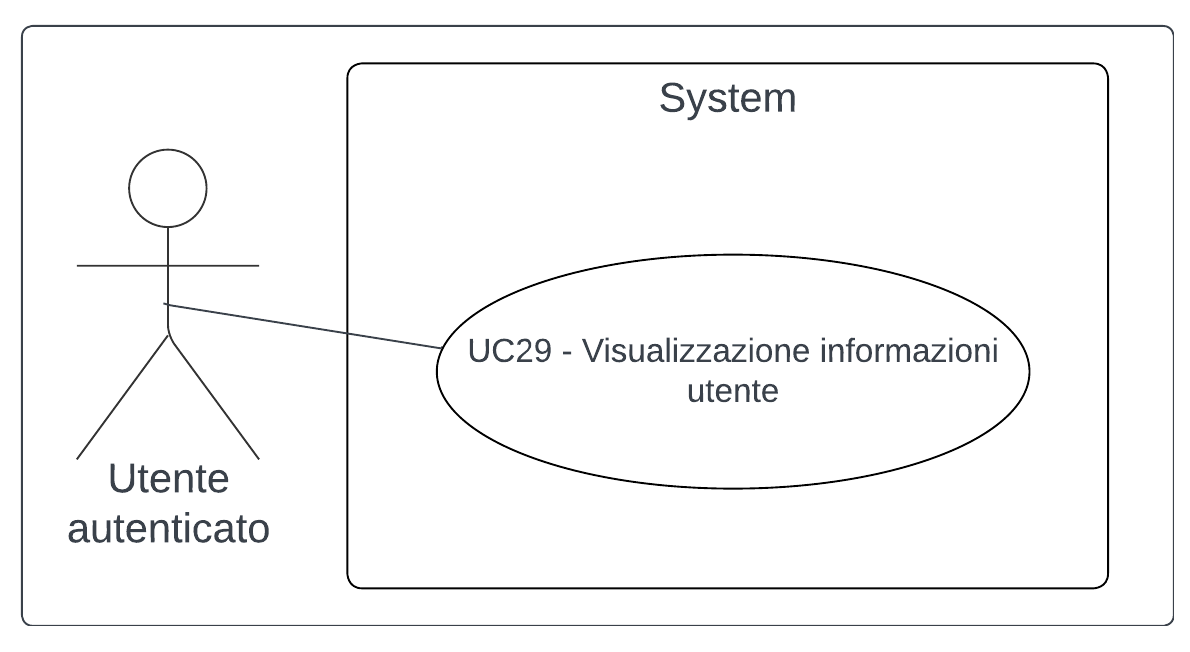
\includegraphics[width=0.9\linewidth]{ucd/UCD29.png}
\end{figure}
\textbf{Attori}:
\begin{itemize}
    \item Utente autenticato
\end{itemize}
\textbf{Precondizioni}:
\begin{itemize}
    \item L'utente ha già creato il suo account
\end{itemize}
\textbf{Postcondizioni}:
\begin{itemize}
    \item L'utente visualizza le informazioni del suo profilo
\end{itemize}
\textbf{Scenario principale}:
\begin{enumerate}
    \item L'utente visualizza le informazioni:
    \begin{enumerate}
        \item Nome
        \item Cognome
        \item Email associata
        \item (Immagine profilo)
        \item Recensioni effettuate
    \end{enumerate}
    \item Se l'utente è amministratore di un ristorante visualizza \nameref{usecase:29_1}
\end{enumerate}
\begin{comment}
\subsubsection{UC29.1 - Visualizzazione informazioni ristorante}\label{usecase:29_1}
\textbf{Attori}:
\begin{itemize}
    \item Amministratore.
\end{itemize}
\textbf{Precondizioni}:
\begin{itemize}
    \item L'utente ha già creato e possiede un suo account;
    \item L'utente è amministratore di un ristorante.
\end{itemize}
\textbf{Postcondizioni}:
\begin{itemize}
    \item L'utente visualizza le informazioni del suo profilo.
\end{itemize}
\textbf{Scenario principale}:
\begin{enumerate}
    \item L'utente visualizza le informazioni:
    \begin{enumerate}
        \item Nome ristorante;
        \item Tipologia di cucina del ristorante;
        \item Posti totali.
    \end{enumerate}
\end{enumerate}
\end{comment}
\newpage
%case d'uso 30 Interazione con il cliente
\begin{comment}
\subsection{UC30 - Visualizzazione ristoranti (per amministratore)}\label{usecase:30}

\begin{figure}[H]
    \centering
    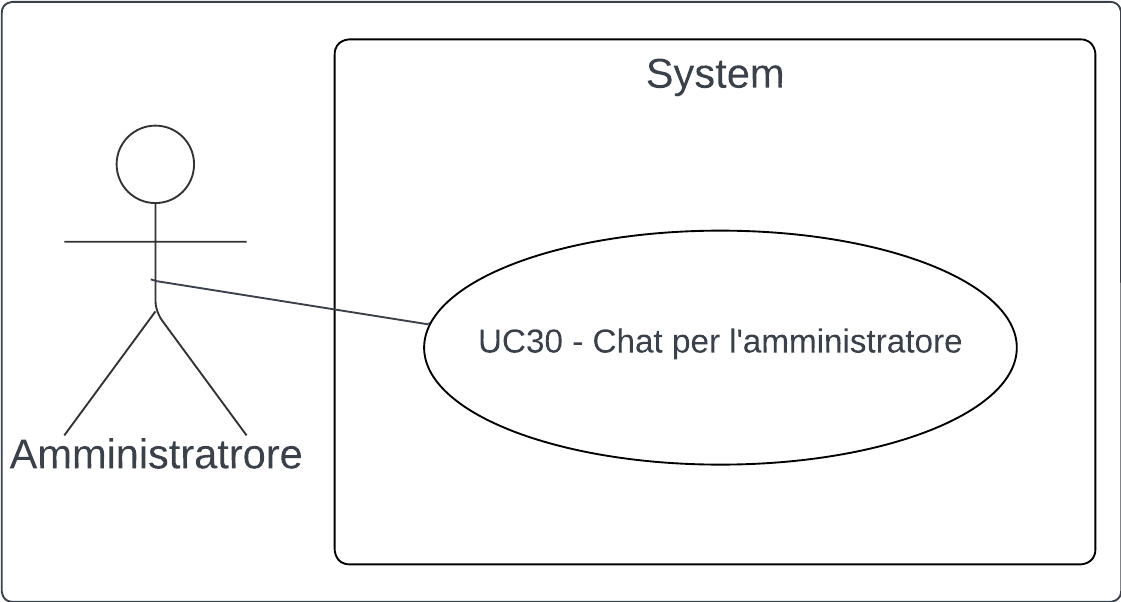
\includegraphics[width=0.9\linewidth]{ucd/UCD30.png}
\end{figure}

\textbf{Attori}:
\begin{itemize}
    \item \textit{Amministratore}_G
\end{itemize}
\textbf{Precondizioni}:
\begin{itemize}
    \item L'amministratore è autenticato nel sistema
\end{itemize}
\textbf{Postcondizioni}:
\begin{itemize}
    \item L'amministratore ha visualizzato l'elenco dei ristoranti
\end{itemize}
\textbf{\textit{Scenario}_G principale}:
\begin{enumerate}
    \item L'amministratore seleziona l'opzione per visualizzare l'elenco dei ristoranti di cui è l'amministratore
    \item Il sistema visualizza l'elenco dei ristoranti
\end{enumerate}
\textbf{Scenari alternativi}:\\
\textit{Nessun ristorante registrato}:
\begin{enumerate}
    \item Dopo il recupero dell'elenco dei ristoranti, il sistema non trova alcun ristorante registrato
    \item Il sistema visualizza un messaggio all'amministratore indicando che non ci sono ristoranti registrati nel sistema
\end{enumerate}

\newpage
\end{comment}
\subsection{UC30 - Chat per l'amministratore}\label{usecase:30}
\begin{figure}[H]
    \centering
    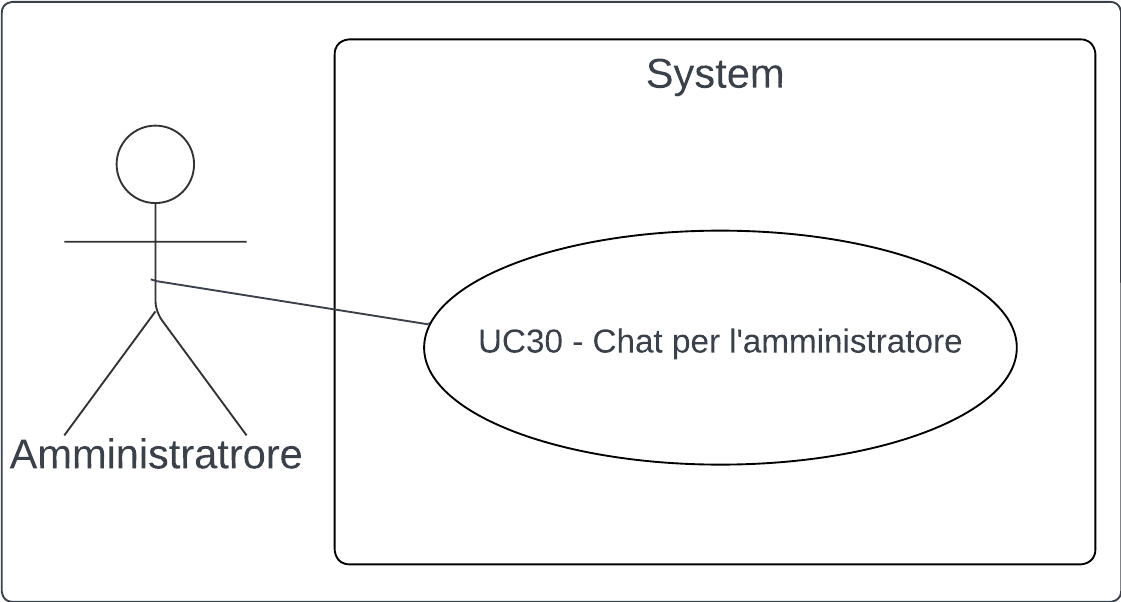
\includegraphics[width=0.75\linewidth]{ucd/UCD30.png}
\end{figure}
\textbf{Attori}:
\begin{itemize}
    \item \textit{Amministratore}_G
\end{itemize}
\textbf{Precondizioni}:
\begin{itemize}
    \item L'amministratore amministra un ristorante
\end{itemize}
\textbf{Postcondizioni}:
\begin{itemize}
    \item L'amministratore visualizza una chat per rispondere ad eventuali utenti che hanno scritto
\end{itemize}
\textbf{\textit{Scenario}_G principale}:
\begin{enumerate}
    \item L'amministratore visualizza una lista di chat che gli utenti hanno aperto
    \item Seleziona una chat
    \item Visualizza il testo
    \item L'amministratore può rispondere tramite testo
\end{enumerate}
\textbf{Scenari alternativi}:
\begin{enumerate}
    \item Il testo inserito è:
    \begin{enumerate}
        \item Vuoto
        \item Troppo lungo
    \end{enumerate}
    \item L'invio viene annullato e viene visualizzato un errore
\end{enumerate}
\newpage
% $\textit{caso d'uso}_G$ 31 Modifica menu' del ristorante
\subsection{UC31 - Modifica menu' del ristorante}\label{usecase:31}
\begin{figure}[H]
    \centering
    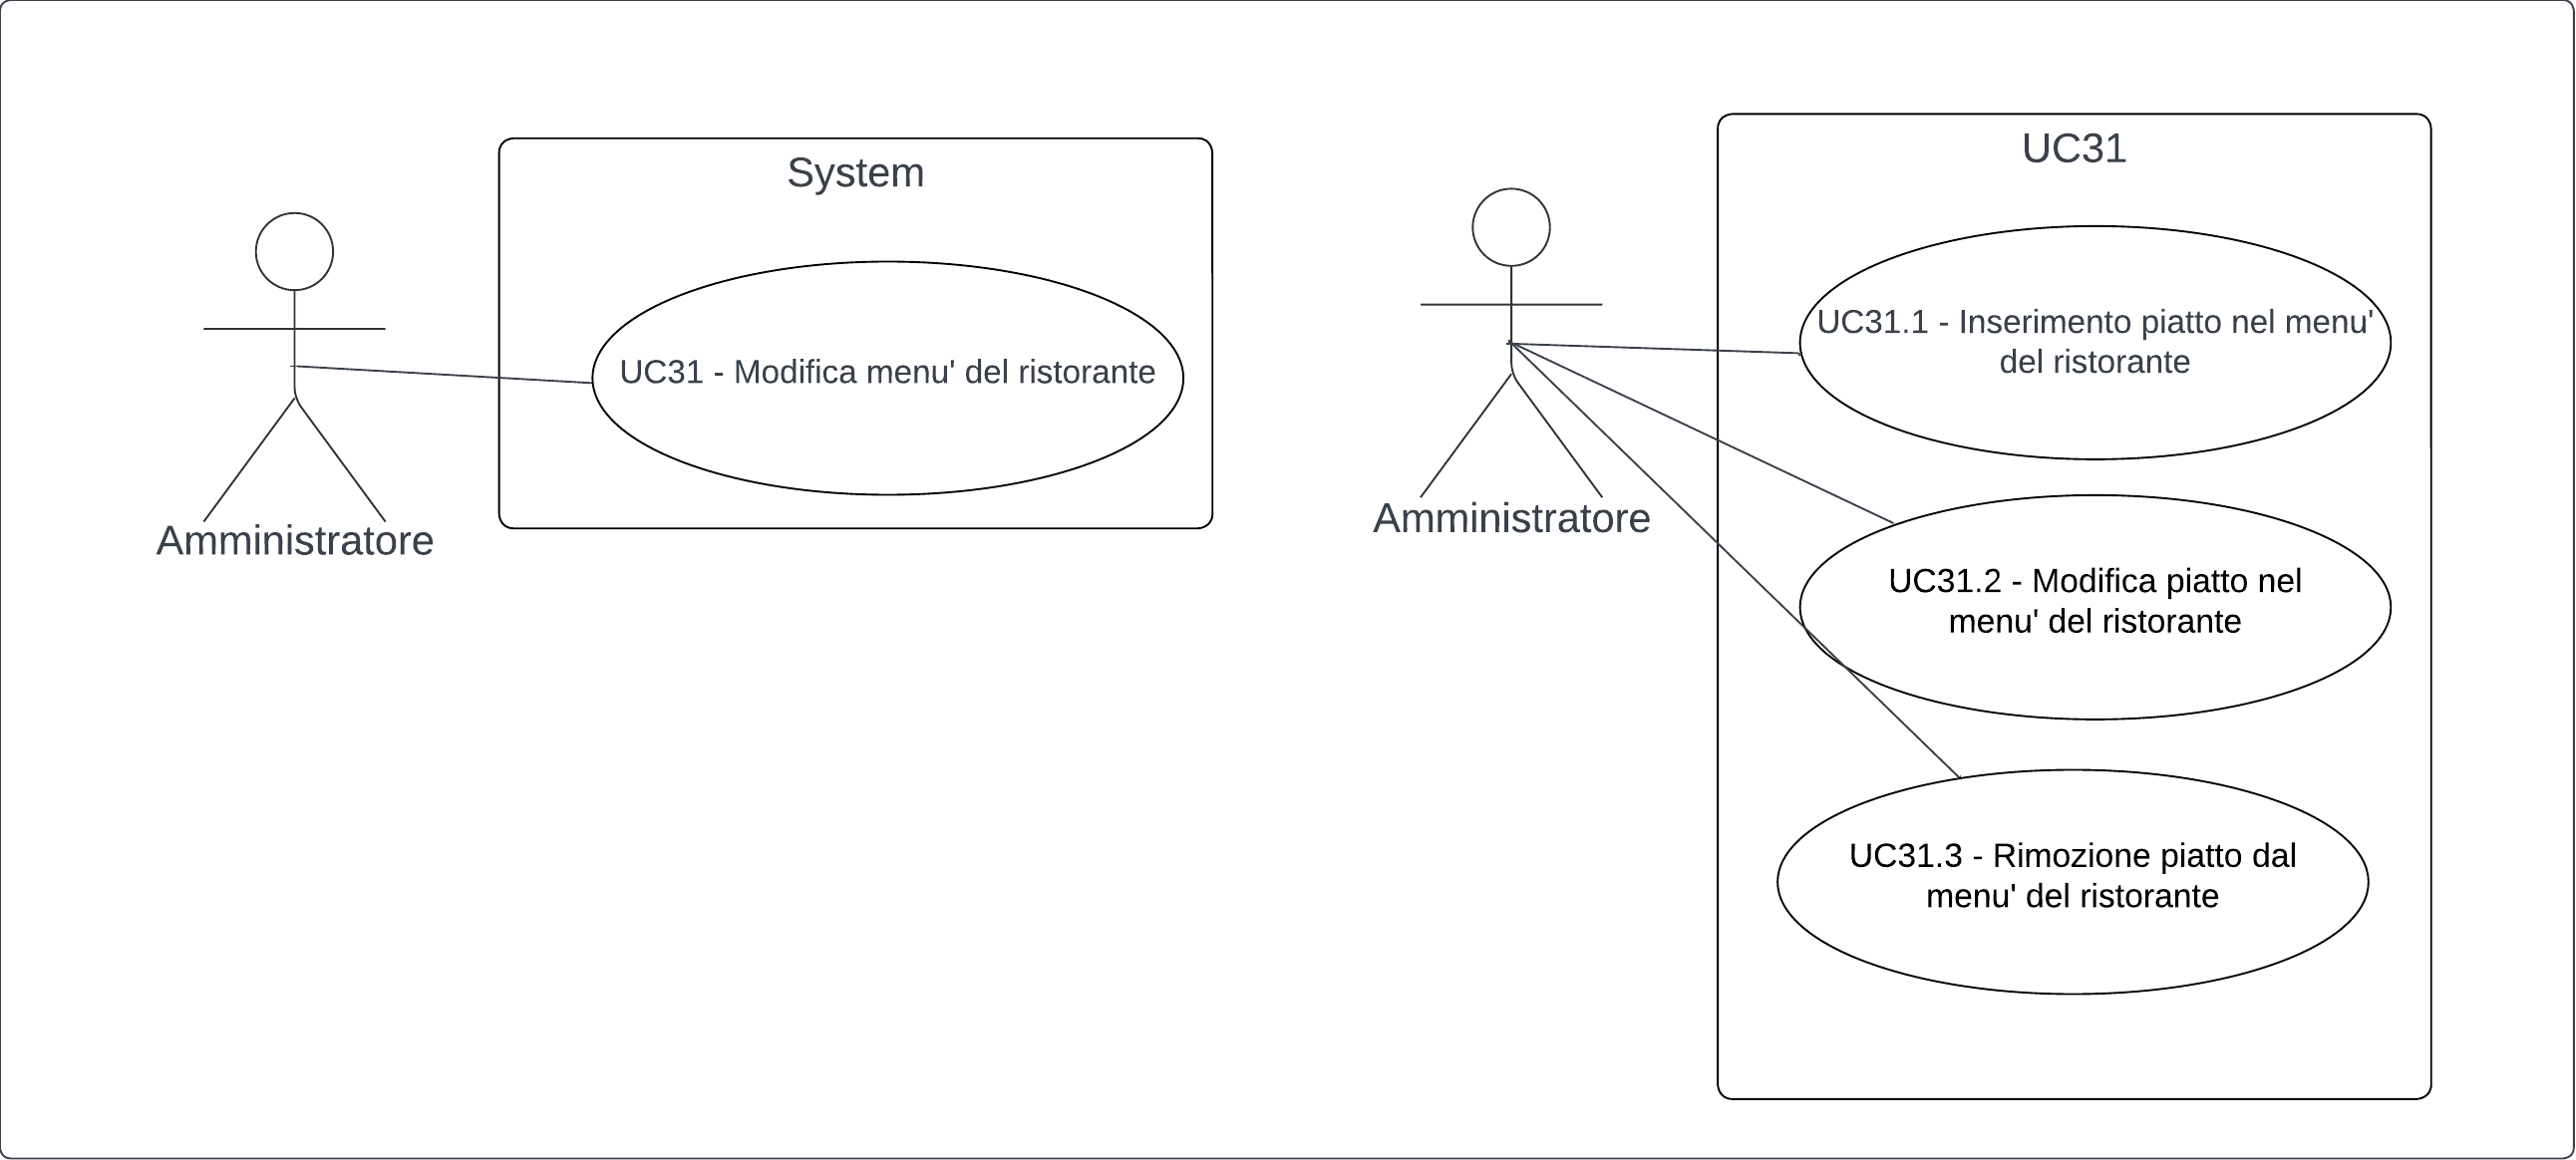
\includegraphics[width=0.9\linewidth]{ucd/UCD31.png}
\end{figure}
\textbf{Attori}:
\begin{itemize}
    \item Amministratore
\end{itemize}
\textbf{Precondizioni}:
\begin{itemize}
    \item L'utente ha inserito le informazioni sul proprio ristorante (\nameref{usecase:2_1})
\end{itemize}
\textbf{Postcondizioni}:
\begin{itemize}
    \item L'utente ha modificato il menu' del proprio ristorante
\end{itemize}
\textbf{Scenario principale}:
\begin{enumerate}
    \item L'utente può compiere le seguenti azioni per gestire il menu'
    \begin{enumerate}
        \item Inserire un piatto nel menu' (\nameref{usecase:31_1})
        \item Modificare un piatto nel menu' (\nameref{usecase:31_2})
        \item Rimuovere un piatto dal menu' (\nameref{usecase:31_3})
    \end{enumerate}
    \item L'utente conferma le modifiche e il \textit{Sistema_G} le registra
\end{enumerate}

%caso d'uso 31.1 Inserimento piatto nel menu' del ristorante
\newpage
\subsubsection{UC31.1 - Inserimento piatto nel menu' del ristorante}\label{usecase:31_1}
\textbf{Attori}:
\begin{itemize}
    \item Amministratore.
\end{itemize}
\textbf{Precondizioni}:
\begin{itemize}
    \item L'utente è connesso al sistema.
\end{itemize}
\textbf{Postcondizioni}:
\begin{itemize}
    \item L’utente ha aggiunto un piatto al menu’ del ristorante.
\end{itemize}
\textbf{Scenario principale}:
\begin{enumerate}
    \item L'utente inserisce le informazioni relative ad una nuova pietanza da inserire nel menu':
    \begin{itemize}
        \item L'utente inserisce il nome della pietanza;
        \item L'utente inserisce gli ingredienti che compongono tale pietanza;
        \item L'utente inserisce il prezzo relativo a tale pietanza;
    \end{itemize}
    \item L'utente conferma le modifiche che verranno applicate al menu' del ristorante.
\end{enumerate}
\textbf{Scenari alternativi}: 
\begin{enumerate}
    \item L'utente inserisce un nome di un piatto già presente nel menu';
    \item L'utente visualizza un messaggio di errore.
\end{enumerate}

%caso d'uso 31.2 Modifica piatto del menu' del ristorante
\subsubsection{UC31.2 - Modifica piatto del menu' del ristorante}\label{usecase:31_2}
\textbf{Attori}:
\begin{itemize}
    \item Amministratore
\end{itemize}
\textbf{Precondizioni}:
\begin{itemize}
    \item L'utente ha inserito le informazioni sul proprio ristorante (\nameref{usecase:2_1})
    \item L'utente ha già inserito le informazioni del piatto di cui vuole modificare le informazioni (\nameref{usecase:31_1})
\end{itemize}
\textbf{Postcondizioni}:
\begin{itemize}
    \item L'utente ha modificato le informazioni relative ad un piatto presente nel menu' del ristorante
\end{itemize}
\textbf{Scenario principale}:
\begin{enumerate}
    \item L'utente sceglie un piatto presente nel menu' del ristorante
    \item L'utente modifica le informazioni inerenti al piatto
    \item L'utente può modificare:
    \begin{itemize}
        \item il nome del piatto in modo che sia comunque diverso dal nome degli altri piatti
        \item gli ingredienti associati a tale piatto
        \item il prezzo associato a tale piatto
    \end{itemize}
    \item L'utente conferma le modifiche
\end{enumerate}
\textbf{Scenari alternativi}:
\begin{enumerate}
    \item L’utente inserisce un nome di un piatto già presente nel menu’
    \item L'utente visualizza un messaggio di errore
\end{enumerate}

%caso d'uso 31.3 Eliminazione piatto del menu' del ristorante
\subsubsection{UC31.3 - Rimozione piatto del menu' del ristorante}\label{usecase:31_3}
\textbf{Attori}:
\begin{itemize}
    \item Amministratore.
\end{itemize}
\textbf{Precondizioni}:
\begin{itemize}
    \item L'utente è connesso al sistema.
    \item L'utente ha già inserito le informazioni del piatto che vuole rimuovere (\nameref{usecase:31_1}).
\end{itemize}
\textbf{Postcondizioni}:
\begin{itemize}
    \item L'utente ha rimosso un piatto dal menu' del ristorante.
\end{itemize}
\textbf{Scenario principale}:
\begin{enumerate}
    \item L'utente seleziona un piatto da rimuovere nel menu' del ristorante;
    \item Il piatto viene rimosso dal menu';
    \item L'utente conferma le modifiche.
\end{enumerate}
\newpage

%
% INIZIO ERRORI
%

%caso d'uso E1 - Visualizzazione errore $\textit{feedback}_G$ non inserito
%\input{uc/ucE1}

%\input{uc/ucE2}

% Requisiti
\section{Requisiti}
In questa sezione sono stilati i requisiti ottenuti in fase di analisi e derivanti da casi d'uso, il $\textit{capitolato}_G$ d'appalto e verbali sia interni che esterni. 
\subsection{Terminologia}
I requisiti sono identificati dal seguente formato di codice:
\[
\text{R[Priorità][Tipo] [Id]}
\]

Dove:
\begin{itemize}
    \item \textbf{R} sta per "$\textit{Requisito}_G$";
    \item \textbf{Priorità} può essere:
    \begin{itemize}
        \item O (obbligatorio): ovvero un $\textit{requisito}_G$ che deve essere necessariamente soddisfatto alla fine della buona riuscita del progetto;
        \item D (desiderabile): ovvero un $\textit{requisito}_G$ che è apprezzato dal committente ma che non compromette il progetto.
    \end{itemize}
    \item \textbf{Tipo} può essere:
    \begin{itemize}
        \item F (funzionale): ovvero un $\textit{requisito}_G$ che indica una funzionalità del $\textit{sistema}_G$ e che ne definisce il comportamento;
        \item Q (qualità): ovvero un $\textit{requisito}_G$ che definisce le caratteristiche di qualità del prodotto $\textit{software}_G$;
        \item V (vincolo): specifica i limiti e le restrizioni imposte dal $\textit{capitolato}_G$ e dal committente.
    \end{itemize}
    \item \textbf{Id} rappresenta un numero progressivo che identifica il $\textit{requisito}_G$ appartenente ad una tipologia.
\end{itemize}
\newpage
\subsection{Requisiti funzionali}
La seguente sezione dettaglia i requisiti funzionali, delineando le varie funzionalità del $\textit{sistema}_G$, ovvero le azioni eseguibili dallo stesso e le informazioni che il $\textit{sistema}_G$ è in grado di fornire. La presenza di ciascun $\textit{requisito}_G$ è giustificata attraverso l'indicazione della fonte, che può essere un $\textit{caso d'uso}_G$ (UC) specifico o essere derivata direttamente dal testo del $\textit{capitolato}_G$ d'appalto.
In questa sezione i requisiti si suddividono in:
\begin{itemize}
    \item ROF: $\textit{requisiti obbligatori funzionali}_G$.
    \item RDF: $\textit{requisiti desiderabili funzionali}_G$.
\end{itemize}

\begin{longtable}{|c|p{14cm}|p{2cm}|}
    \hline
    \emph{Codice} & \centering{\emph{Descrizione}} &  \emph{Fonte} \\
    \hline
    \endfirsthead
    \endhead

    ROF 1&  L'utente deve poter selezionare un piatto dalla lista dei piatti disponibili.  & UC3.1, UC9  \\
    \hline
    RDF 2& Il $\textit{sistema}_G$ deve inviare una notifica se l'utente base sta aggiungendo un piatto che contiene elementi a cui è allergico/intollerante. & UC3\\
    \hline
    ROF 3& L'utente deve visualizzare i pasti con i loro ingredienti e può modificarli, togliendo o modificandone la quantità. & UC3\\
    \hline
    ROF 4& L'utente base deve essere in grado di visualizzare il riepilogo di quanto ordinato e di confermare. & UC3 \\
    \hline
    ROF 5& Il $\textit{sistema}_G$ deve poter inviare una notifica di conferma dell’ordinazione collaborativa all’amministratore del ristorante.& UC3 \\
    \hline
    ROF 6& L'utente deve poter inserire le informazioni (data, orario, persone) per effettuare una $\textit{prenotazione}_G$. & UC23\\
    \hline
    ROF 7& Il $\textit{sistema}_G$ deve poter inviare una notifica all’amministratore per comunicare la richiesta di $\textit{prenotazione}_G$, che può accettare e rifiutare. & UC23\\
    \hline
    RDF 8& L'utente deve poter essere in grado di cancellare la $\textit{prenotazione}_G$. & UC13, UC23 \\
    \hline
    ROF 9& Il $\textit{sistema}_G$ deve poter negare la $\textit{prenotazione}_G$ se il ristorante non possiede abbastanza posti o tavoli. & UC23 \\
    \hline
    ROF 10& L'utente base deve poter visualizzare una lista di ristoranti filtrata per nome oppure data, luogo, tipologia cucina. & UC24 \\
    \hline
    ROF 11& L'utente base deve poter selezionare un ristorante.  & UC4, UC23 \\
    \hline
    ROF 12& L'amministratore deve essere in grado di poter visualizzare una lista di prenotazioni in attesa. & UC19, UC20 \\
    \hline
    ROF 13& L'amministratore deve poter selezionare una specifica richiesta di $\textit{prenotazione}_G$ dalla lista visualizzata. & UC19, UC20 \\
    \hline
    ROF 14& L'amministratore deve poter accettare la richiesta di $\textit{prenotazione}_G$ selezionata. & UC19 \\
    \hline
    ROF 15& Il $\textit{sistema}_G$, dopo l'accettazione, aggiunge nell'area "prenotazioni" dell'utente la $\textit{prenotazione}_G$. & UC19 \\
    \hline
    ROF 16& Il $\textit{sistema}_G$ deve notificare gli utenti coinvolti (nel caso di $\textit{prenotazione}_G$ collaborativa) l'accettazione della $\textit{prenotazione}_G$. & UC19 \\
    \hline
    RDF 17& Il $\textit{sistema}_G$ deve fornire un'interfaccia per consentire all'amministratore di verificare la disponibilità di posti in base alle specifiche della $\textit{prenotazione}_G$ selezionata. & UC19, UC20 \\
    \hline
    RDF 18& Il $\textit{sistema}_G$ deve ridurre il numero di posti disponibili in base alle specifiche della $\textit{prenotazione}_G$ dopo che questa è stata accettata. & UC19 \\
    \hline
    ROF 19& L'amministratore deve poter rifiutare la richiesta di $\textit{prenotazione}_G$ selezionata. & UC20 \\
    \hline
    ROF 20& Il $\textit{sistema}_G$ deve notificare gli utenti coinvolti (nel caso di $\textit{prenotazione}_G$ collaborativa) del rifiuto della $\textit{prenotazione}_G$. & UC20 \\
    \hline
    RDF 21& Il $\textit{sistema}_G$ deve creare un canale di comunicazione tra l'utente e l'amministratore del ristorante quando l'utente lo richiede. & UC4 \\
    \hline
    RDF 22& L'utente e l'amministratore devono poter scambiare messaggi in modo bidirezionale tramite l'interfaccia di comunicazione. & UC4, UC30 \\
    \hline
    RDF 23& Durante la comunicazione, il $\textit{sistema}_G$ deve inviare notifiche $\textit{push}_G$ per informare l'utente e l'amministratore dei nuovi messaggi ricevuti. & UC4, UC30 \\
    \hline
    ROF 24&  La cancellazione della $\textit{prenotazione}_G$ può essere effettuata con al massimo un giorno di anticipo rispetto alla data della $\textit{prenotazione}_G$.  & UC13 \\ 
    \hline
    ROF 25& Il $\textit{sistema}_G$ deve permettere di pagare il conto in base alla modalità scelta (divisione equa, divisione proporzionale) da chi ha creato la $\textit{ordinazione}_G$ collaborativa. & UC5, UC5.1, UC5.2 \\
    \hline
    RDF 26& L'utente base può pagare l'intero conto se nessun utente non ha ancora effettuato il pagamento. & UC5.3 \\
    \hline
    RDF 27& L'amministratore deve poter essere in grado di modificare il menu' del proprio ristorante, aggiungendo, rimuovendo pietanze e modificando le informazioni del singolo piatto (nome, ingredienti e prezzo). & UC31 \\
    \hline
    RDF 28& La modifica del menu' da parte dell'amministratore non deve causare problemi di sincronizzazione nella visualizzazione, ricerca del menu' e nell'$\textit{ordinazione}_G$ da parte dell'utente base. &  UC3, UC11, UC31 \\
    \hline
    RDF 29& Si deve permettere all'utente base di poter inserire un coupon prima di pagare il conto, che, se applicato, deve far ricalcolare al $\textit{sistema}_G$ il prezzo del conto. & UC18 \\
    \hline

    ROF 30& Il $\textit{sistema}_G$ deve consentire all'amministratore di visualizzare la lista delle prenotazioni effettuate per il proprio ristorante. & UC6, UC15 \\
    \hline
    ROF 31& L'amministratore deve poter visualizzare i dettagli di una specifica $\textit{prenotazione}_G$. & UC6 \\
    \hline
    RDF 32& L'amministratore deve poter visualizzare lo stato delle ordinazioni associate alla $\textit{prenotazione}_G$. & UC6 \\
    \hline
    RDF 33& Il $\textit{sistema}_G$ deve fornire all'amministratore la possibilità di visualizzare la lista totale degli ingredienti inclusi nella $\textit{prenotazione}_G$. & UC6 \\
    \hline
    ROF 34& Il $\textit{sistema}_G$ deve consentire all'amministratore di visualizzare tutti gli ordini confermati per il ristorante selezionato. & UC15 \\
    \hline
    RDF 35& Il $\textit{sistema}_G$ deve permettere di annullare l'$\textit{ordinazione}_G$ collaborativa nel tempo utile per farlo & UC28 \\
    \hline
    RDF 36& Il $\textit{sistema}_G$ invia una notifica a tutti gli utenti associati alla $\textit{prenotazione}_G$ la cui $\textit{ordinazione}_G$ collaborativa è stata annullata & UC28 \\
    \hline
    ROF 37& Il $\textit{sistema}_G$ deve fornire un'interfaccia per consentire agli utenti non autenticati di registrarsi come utenti base. & UC1 \\
    \hline
    ROF 38& L'utente/L'amministratore deve poter inserire le sue informazioni personali durante la registrazione come nome, cognome, email, password. & UC1, UC2 \\
    \hline
    ROF 39& L'utente/L'amministratore deve poter confermare di volersi registrare con le informazioni fornite prima di completare la registrazione. & UC1, UC2 \\
    \hline
    ROF 40& Il $\textit{sistema}_G$ deve gestire correttamente gli errori nell'inserimento delle informazioni durante la registrazione. & UC1, UC2 \\
    \hline 
    ROF 41& L'utente base e l'amministratore devono poter visualizzare il menu' del ristorante selezionato & UC3, UC11\\
    \hline
    RDF 42& L'amministratore deve poter modificare le informazioni del proprio ristorante (nome, indirizzo, orari, coperti e tipologia di cucina) & UC14\\
    \hline
    RDF 43& La modifica delle informazioni del ristorante da parte dell'amministratore non deve causare problemi di sincronizzazione nella visualizzazione, ricerca del ristorante e nell'$\textit{ordinazione}_G$ da parte dell'utente base & UC3, UC14 \\
    \hline
    RDF 44& L'utente autenticato deve poter visualizzare una lista con le prenotazioni passate & UC17 \\
    \hline
    RDF 45& L'utente autenticato deve poter rilasciare una recensione (con anche una votazione di gradimento tramite stelle) sui ristoranti nei quali ha effettuato almeno una $\textit{prenotazione}_G$ & UC7 \\
    \hline
    ROF 46& L'utente autenticato deve poter visualizzare gli ordini di un tavolo & UC8 \\
    \hline
    RDF 47& L'utente autenticato deve poter visualizzare le recensioni rilasciate ed eventualmente eliminarle & UC10 \\
    \hline
    RDF 48& L'utente generico può visualizzare le recensioni di un ristorante e visualizzare per ognuna di essa le relative informazioni & UC21 \\
    \hline
    ROF 49& L'amministratore deve poter inserire le informazioni del ristorante di cui è amministratore & UC2 \\
    \hline
    ROF 50& L'utente/L'amministratore deve poter inserire la propria email e la password durante la fase di login.  & UC12 \\
    \hline
    ROF 51& Il $\textit{sistema}_G$ deve verificare che le informazioni inserite nel login corrispondano ad un account già esistente nel $\textit{sistema}_G$.  & UC12 \\
    \hline
    RDF 52& Il $\textit{sistema}_G$ deve predisporre un’opzione per il recupero della password.  & UC12 \\
    \hline
    RDF 53& L’utente non autenticato deve poter inserire la propria email durante il $\textit{processo}_G$ di recupero password.  & UC16 \\
    \hline
    RDF 54 & Se l’email inserita dall’utente corrisponde ad un account nel $\textit{sistema}_G$, il $\textit{sistema}_G$ deve inviare un’email contenente un link per il recupero della password.  & UC16 \\
    \hline
    ROF 55 & Se l'email inserita dall'utente non corrisponde a un account nel $\textit{sistema}_G$, il $\textit{sistema}_G$ lo mostra a schermo.  & UC16 \\
    \hline
    RDF 56 & L’utente deve poter accedere a una sezione dedicata per il recupero della password tramite il link fornito nell’email di recupero password.  & UC16 \\
    \hline
    ROF 57 & Il $\textit{sistema}_G$ deve mostrare una lista di prenotazioni per l'utente base, ognuna con le seguenti informazioni:
    nome del ristorante, data, ora, stato della $\textit{prenotazione}_G$ (se è ancora attiva o già completata) e numero di persone coinvolte. & UC17 \\
    \hline
    RDF 58 & Il $\textit{sistema}_G$ ordina la lista delle prenotazioni per data della $\textit{prenotazione}_G$.  & UC17 \\
    \hline

    RDF 59 & L'utente base deve poter inserire le proprie allergie/intolleranze, se presenti, durante la modifica del profilo.  & UC25  \\
    \hline

    RDF 60 & L’utente autenticato e l’amministratore devono poter inserire nome, cognome, email e password nell’area di modifica delle proprie informazioni.  & UC26  \\
    \hline
    ROF 61 & Il $\textit{sistema}_G$ deve verificare che l'email inserita dall'utente autenticato sia valida e non sia già presente nel $\textit{sistema}_G$.  & UC26  \\
    \hline
    ROF 62 & L'utente base autenticato deve poter accedere alla funzionalità di $\textit{ordinazione}_G$ di un piatto.  & UC3.1  \\
    \hline
    ROF 63 & Il $\textit{sistema}_G$ deve consentire all'utente di visualizzare e togliere ingredienti del piatto selezionato.  & UC3.1, UC9  \\
    \hline
    RDF 64 & L'amministratore deve poter visualizzare le recensioni del proprio ristorante. & UC22 \\ 
    \hline
    RDF 65 & L'amministratore deve poter rispondere alle recensioni del proprio ristorante. & UC22 \\
    \hline
    RDF 66 & L'utente deve poter visualizzare le risposte alla propria recensione. & UC22 \\
    \hline
    ROF 67 & Il $\textit{sistema}_G$ deve poter consentire di modificare l'ordine ad un utente prima della scadenza del tempo previsto, inserendo piatti, modificando ingredienti e quantità delle pietanze ordinate. & UC9 \\
    \hline
    RDF 68 & Il $\textit{sistema}_G$ permette di far visualizzare all'amministratore il dettaglio degli ingredienti necessari per ogni giornata. & UC15 \\
    \hline
    ROF 69 & Il $\textit{sistema}_G$ deve consentire all'utente autenticato di accedere alla funzionalità di logout. & UC27 \\
    \hline
    RDF 70 & Dopo che l'utente ha selezionato l'opzione di logout, il $\textit{sistema}_G$ deve richiedere una conferma esplicita dall'utente prima di procedere con la disconnessione. & UC27 \\ 
    \hline
    ROF 71 & Dopo aver terminato la sessione dell'utente, il $\textit{sistema}_G$ deve reindirizzare l'utente alla pagina di accesso o a una pagina di destinazione predefinita. & UC27 \\
    \hline
    RDF 72 & L'utente autenticato deve poter visualizzare le informazioni del suo profilo. & UC29 \\ 
    \hline

    RDF 73 & L'amministratore deve poter visualizzare tutte le chat aperte in precedenza da altri utenti. & UC30 \\
    \hline
    RDF 74 & L'amministratore deve poter rispondere ai messaggi inviati da gli utenti & UC30 \\
    \hline
    ROF 75 & Il $\textit{sistema}_G$ deve poter generare un link di invito per la $\textit{prenotazione}_G$ & UC23 \\
    \hline
    ROF 76 & Il $\textit{sistema}_G$ permette di far visualizzare all'amministratore la lista totale degli ingredienti necessari per soddisfare la singola $\textit{prenotazione}_G$. & UC15 \\
     \hline
    ROF 77 & Il $\textit{sistema}_G$ invia una notifica all’amministratore in base agli
    aggiornamenti sul conto di una $\textit{prenotazione}_G$ del suo ristorante. & UC5 \\
     \hline
\caption{Requisiti funzionali}
\end{longtable}

\subsection{Requisiti di qualità}
Questa sezione delinea le specifiche qualitative che devono essere rispettate per garantire la qualità del $\textit{sistema}_G$.
\begin{longtable}{|c|p{14cm}|p{2cm}|}
    \hline
    \emph{Codice} & \centering{\emph{Descrizione}} &  \emph{Fonte} \\
    \hline
    \endfirsthead
    \endhead
    ROQ 1&  Il codice sorgente deve essere coperto da $\textit{test}_G$ per almeno l'80\% e ciò deve essere dimostrato tramite report. & $\textit{Capitolato}_G$ \\
    \hline
    ROQ 2 & Deve essere prodotta della documentazione che discuta delle scelte implementative e progettuali riportandone le relative motivazioni. & $\textit{Capitolato}_G$ \\
    \hline
    ROQ 3 & Deve essere prodotta della documentazione che discuta delle problematiche aperte e di eventuali soluzioni soluzioni da esplorare. & $\textit{Capitolato}_G$ \\
    \hline
    RDQ 4 & Deve essere fornita un'analisi rispetto al carico massimo supportato in numero di dispositivi e di quale sarebbe il servizio cloud più adatto per supportarlo analizzando prezzo, stabilità del servizio e assistenza. & $\textit{Capitolato}_G$ \\
    \hline
    ROQ 5 & Devono essere rispettate le norme definite nel documento $\textit{Norme di Progetto}_G$. & $\textit{Verbale}_G$ interno \\
    \hline
    ROQ 6 & Devono essere rispettate le metriche e i vincoli definiti in $\textit{Piano di Qualifica}_G$. & $\textit{Verbale}_G$ interno \\
    \hline
\caption{Requisiti di qualità}
\end{longtable}
    
\subsection{Requisiti di vincolo}
Questa sezione delinea i limiti e le restrizioni che il $\textit{sistema}_G$ deve tenere conto per adempiere alle esigenze del proponente.
\begin{longtable}{|c|p{14cm}|p{2cm}|}
    \hline
    \emph{Codice} & \centering{\emph{Descrizione}} &  \emph{Fonte} \\
    \hline
    \endfirsthead
    \endhead
    ROV 1& L'interfaccia utente deve essere un'$\textit{Applicazione Web Responsive}_G$.  & $\textit{Capitolato}_G$  \\
    \hline
    ROV 2& La struttura del progetto prevede la completa separazione tra \textit{backend} e \textit{frontend}  & $\textit{Verbale}_G$ esterno  \\
    \hline
    ROV 3& L'implementazione del \textit{frontend} è realizzata in \textit{Next.js}  & $\textit{Verbale}_G$ Esterno  \\
    \hline
    ROV 4& L'implementazione del \textit{backend} è realizzata in \textit{NestJS}  & $\textit{Verbale}_G$ Esterno  \\
    \hline
    ROV 5& L'applicazione utilizza \textit{Node.js} versione 21 & $\textit{Verbale}_G$ Interno  \\
    \hline
    ROV 6& Il database è realizzato con \textit{PostgreSQL}  & $\textit{Verbale}_G$ Interno  \\
    \hline
    ROV 7& Le funzionalità che richiedono una comunicazione in tempo reale tra più utenti sono gestite dalla libreria \textit{Socket.IO}  & $\textit{Verbale}_G$ Esterno  \\
    \hline
    ROV 8& $\textit{Architettura}_G$ basata a micro-servizi & $\textit{Verbale}_G$ Interno  \\
    \hline
    ROV 9& I browser supportati sono: \textit{Firefox} 67+; \textit{Chrome} 64+; \textit{Edge} 79+; \textit{Safari} 12+  & $\textit{Verbale}_G$ Interno  \\
    \hline
\caption{Requisiti di vincolo}
\end{longtable}


\setlength{\extrarowheight}{8pt}
\subsection{Tracciamento}
\subsubsection{Fonte - Requisiti}
\begin{longtable}{|p{4cm}|p{12cm}|}
    \hline
    \emph{Fonte} & \emph{Requisiti}\\
    \hline
    \endfirsthead
    \endhead
    $\textit{Capitolato}_G$ & ROQ 1, ROQ 2, ROQ 3, RDQ 4, ROV 1 \\
    \hline
    $\textit{Verbale}_G$ interno & ROQ 5, ROQ 6, ROV 5, ROV 6, ROV 7, ROV 8, ROV 9 \\
    \hline
    $\textit{Verbale}_G$ esterno & ROV 2, ROV 3, ROV 4, ROV 7 \\
    \hline
    UC1 & ROF 37, ROF 38, ROF 39, ROF 40 \\
    \hline
    UC2 & ROF 38, ROF 39, ROF 40, ROF 49  \\
    \hline
    UC3 & RDF 2 , ROF 3, ROF 4, ROF 5, RDF 28, ROF 41, RDF 43 \\
    \hline 
    UC3.1 & ROF1, ROF 62, ROF 63 \\
    \hline
    UC4 & ROF 11, RDF 21, RDF 22, RDF 23 \\
    \hline
    UC5 & ROF 25, ROF 77 \\
    \hline
    UC5.1 & ROF 25 \\
    \hline
    UC5.2 & ROF 25 \\
    \hline
    UC5.3 & RDF 26 \\
    \hline
    UC6 & ROF 30, ROF 31, ROF 32, RDF 33 \\
    \hline
    UC7 & RDF 45  \\
    \hline
    UC8 & ROF 46 \\
    \hline
    UC9 & ROF 1, ROF 63, ROF 67 \\
    \hline
    UC10 & RDF 47 \\
    \hline
    UC11 & RDF 28, ROF 41 \\
    \hline
    UC12 & ROF 50, ROF 51, ROF 52 \\
    \hline
    UC13 & RDF 8, ROF 24 \\
    \hline
    UC14 & RDF 42, RDF 43 \\
    \hline
    UC15 & ROF 30, ROF 34, RDF 68, ROF 76 \\
    \hline
    UC16 & ROF 53, ROF 54, ROF 55, ROF 56 \\
    \hline
    UC17 & RDF 44, ROF 57, RDF 58 \\
    \hline
    UC18 & RDF 29 \\
    \hline
    UC19 & ROF 12, ROF 13, ROF 14, ROF 15, ROF 16, RDF 17, RDF 18 \\
    \hline
    UC20 & ROF 12, ROF 13, RDF 17, ROF 19, ROF 20\\
    \hline
    UC21 & RDF 48 \\
    \hline
    UC22 & RDF 64, RDF 65, RDF 66 \\
    \hline
    UC23 & ROF 6, RDF 7, RDF 8, ROF 9, ROF 11, ROF 75\\
    \hline
    UC24 & ROF 10\\
    \hline
    UC25 & RDF 59 \\
    \hline
    UC26 & ROF 60, ROF 61 \\
    \hline
    UC27 & ROF 69, RDF 70, ROF 71 \\
    \hline
    UC28 & RDF 35, RDF 36 \\
    \hline
    UC29 & RDF 72 \\
    \hline
    UC30 & RDF 22, RDF 23, RDF 73, RDF 74 \\
    \hline
    UC31 & RDF 27, RDF 28 \\
    \hline

\caption{Tracciamento Fonte - Requisiti}
    
\end{longtable}



\begin{comment}

\paragraph{Requisiti di qualità}
\begin{longtable}{|p{4cm}|p{12cm}|}
    \hline
    \emph{Fonte} & \emph{Requisiti}\\
    \hline
    \endfirsthead
    \endhead
    UC1 &  \\
    \hline
\caption{Tracciamento Fonte - Requisiti di qualità}
    
\end{longtable}
\paragraph{Requisiti di vincolo}
\begin{longtable}{|p{4cm}|p{12cm}|}
    \hline
    \emph{Fonte} & \emph{Requisiti}\\
    \hline
    \endfirsthead
    \endhead
    UC1 &  \\
    \hline
\caption{Tracciamento Fonte - Requisiti di vincolo}
    
\end{longtable}
         ROF 84 & L'amministratore deve poter visualizzare le informazioni del proprio ristorante & UC29.1 \\
    \hline
    ROF 1 & L'utente base deve poter visualizzare i pasti ordinabili & UC3, UC11\\
    \hline

    RDF 2 & L'utente base deve poter inserire dei parametri per filtrare i pasti ordinabili  & UC3 \\
    \hline
    ROF 72 & L'utente deve poter selezionare un piatto dalla lista dei piatti disponibili.  & UC3.1, UC9  \\
    \hline
     ROF 68 & L'utente autenticato deve poter accedere alla funzionalità di modifica delle proprie informazioni utente.  & UC26  \\
    \hline
         ROF 66 & L'utente autenticato deve poter accedere alla funzionalità di modifica del proprio profilo  & UC25 \\
    \hline
    ROF 36 & L'amministratore deve poter consultare il proprio ristorante e le prenotazioni associate. & UC6, UC15 \\
    \hline
    ROF 28 & L'utente base deve poter ricercare un ristorante per nome & UC24 \\
    \hline
    ROF 29 & L'utente base deve poter ricercare un ristorante per data e luogo, tipologia cucina & UC24 \\
    \hline
    ROF 30 & L'utente base deve poter visualizzare una lista dei ristoranti come risultato della ricerca & UC24 \\
    \hline
    ROF 23 & Il $\textit{sistema}_G$ deve permettere all'utente di effettuare una ricerca dei ristoranti disponibili. & UC4 \\
    \hline
\end{comment}

\end{document}